\documentclass[a4paper]{book}
%\special{dvipdfmx:config z 0} %取消PDF压缩,加快速度,最终版本生成的时候最好把这句话注释掉

\usepackage{amssymb}
\usepackage{bookmark}
\usepackage[hypcap=false]{caption}
\usepackage{enumitem}	% 定制enumerate标号
\usepackage{geometry}
\geometry{
	left=2cm,
	right=2cm,
	top=2cm,
	bottom=2cm,
}
\usepackage{hyperref}
\hypersetup{
    colorlinks=true,            %链接颜色
    linkcolor=black,             %内部链接
    filecolor=magenta,          %本地文档
    urlcolor=cyan,              %网址链接
}
\usepackage[none]{hyphenat}		% 阻止长单词分在两行
\usepackage{mathrsfs}
\usepackage[version=4]{mhchem}
\usepackage{subcaption}
\usepackage{titlesec}

% setting about showing the contents
\setcounter{tocdepth}{3}
\setcounter{chapter}{5}

\RequirePackage[many]{tcolorbox}
\tcbset{
    boxed title style={colback=magenta},
	breakable,
	enhanced,
	sharp corners,
	attach boxed title to top left={yshift=-\tcboxedtitleheight,  yshifttext=-.75\baselineskip},
	boxed title style={boxsep=1pt,sharp corners},
    fonttitle=\bfseries\sffamily,
}

\definecolor{skyblue}{rgb}{0.54, 0.81, 0.94}

\newcounter{exercise}[chapter]
\newcounter{solution}[chapter]
\newcounter{eqs}[solution]

\newenvironment{sequation}
  {\begin{equation}\stepcounter{eqs}\tag{\thesolution-\theeqs}}
  {\end{equation}}

\newtcolorbox[use counter=exercise, number within=chapter, number format=\arabic]{exercise}[1][]{
    title={Exercise~\thetcbcounter},
    colframe=skyblue,
    colback=skyblue!12!white,
    boxed title style={colback=skyblue},
    overlay unbroken and first={
        \node[below right,font=\small,color=skyblue,text width=.8\linewidth]
        at (title.north east) {#1};
    }
    label={\unskip},
    before upper={
        \phantomsection
        \addcontentsline{toc}{subsubsection}{Exercise\hspace{1em}\thetcbcounter}
    },
}

\newtcolorbox[use counter=solution, number within=chapter, number format=\arabic]{solution}[1][]{
    title={Solution~\thetcbcounter},
    colframe=teal!60!green,
    colback=green!12!white,
    boxed title style={colback=teal!60!green},
    overlay unbroken and first={
        \node[below right,font=\small,color=red,text width=.8\linewidth]
        at (title.north east) {#1};
    }
}


% special new commands for common symbols used in the article
\newcommand\tr[1]{\mathrm{tr(#1)}}
\newcommand*{\dif}{\mathop{}\!\mathrm{d}}
\renewcommand\det[1]{\mathrm{det\left(#1\right)}}
\newcommand{\HF}{{\rm HF}}
\newcommand{\corr}{{\rm corr}}

\newcommand{\A}{{\bf A}}
\newcommand{\B}{{\bf B}}
\newcommand{\C}{{\bf C}}
\newcommand{\I}{{\bf 1}}
\newcommand{\U}{{\bf U}}
\newcommand{\HH}{{\bf H}}

\titleformat{\chapter}[display]
  {\bfseries\Large}
  {\filright\MakeUppercase{\chaptertitlename} \Huge\thechapter}
  {1ex}
  {\titlerule\vspace{1ex}\filleft}
  [\vspace{1ex}\titlerule]

% 带*的 sectionstar 格式
\newcommand{\sectionstar}[1]{%
  \stepcounter{section} % 手动增加章节计数器
  \titleformat{\section}
    {\normalfont\Large\bfseries}
    {*\thesection}{1em}{}
  \section*{*\thesection\hspace{1em} #1}
  \addcontentsline{toc}{section}{\protect\numberline{*\thesection}#1}
  \titleformat{\section} % 恢复普通的 section 格式
    {\normalfont\Large\bfseries}
    {\thesection}{1em}{}
}
  
\newcommand\Figref[1]{Fig \ref{#1}}
\newcommand\Tableref[1]{Table \ref{#1}}

\allowdisplaybreaks

\begin{document}

	\tableofcontents

	\chapter{Many-Body Perturbation Theory}
	
	\section{Rayleigh-Schr{\"o}dinger (RS) Perturbation Theory}
	
	\sectionstar{Diagrammatic Representation of RS Perturbation Theory}
	
	\subsection{Diagrammatic Perturbation Theory for Two States}
	
	% 6.1
	\begin{exercise}
	Write down and evaluate all fifth-order diagrams that have the property that an imaginary horizontal line crosses only one hole and one particle line. Show that the sum of such diagrams is
	\[
		\frac{V_{12}V_{21}(V_{22}-V_{11})^3}{(E^{(0)}_1 - E^{(0)}_2)^4}
	\]
	{\it Hint}: There are eight such diagrams, and they can be generated by adding three dots to the second-order diagram in all positive ways.
	\end{exercise}
	
	\begin{solution}
	 
	The final results are listed below firstly. 
	
	\begin{center}
	\begin{tabular}{cccc}
	
		\begin{minipage}{0.22\linewidth}
		\centering
		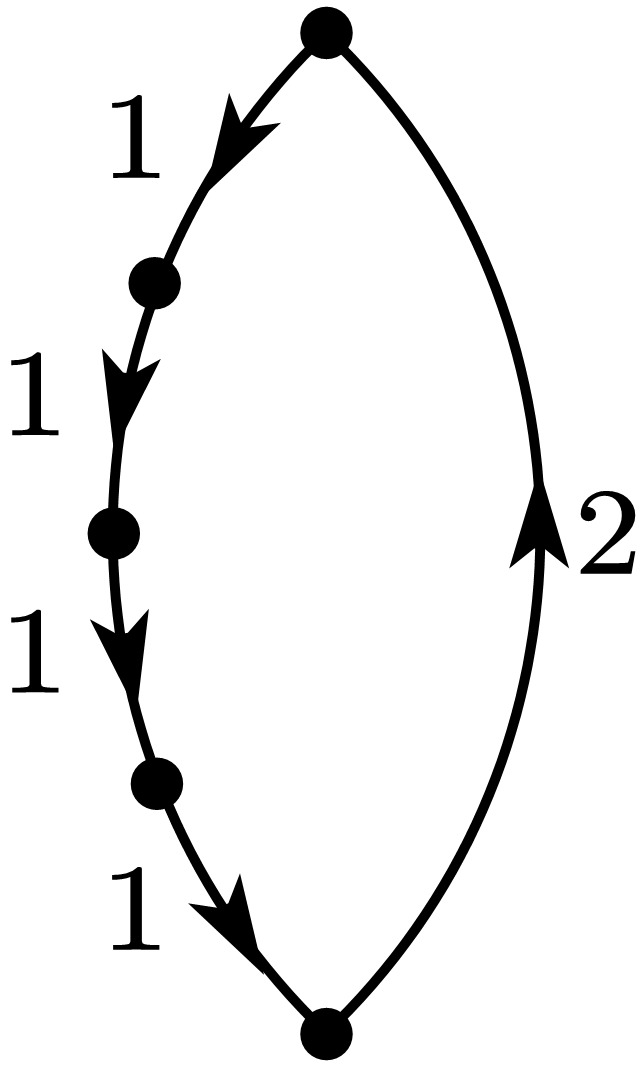
\includegraphics[scale=1.0,trim=0 -4 0 -4]{./pictures/6.01/1.png}
		\captionof*{figure}{$\displaystyle (-1)^{4+1} \frac{ V^3_{11} V_{12} V_{21} }{ ( E^{(0)}_1 - E^{(0)}_2)^4 }$}
		\end{minipage} &
		
		\begin{minipage}{0.22\linewidth}
		\centering
		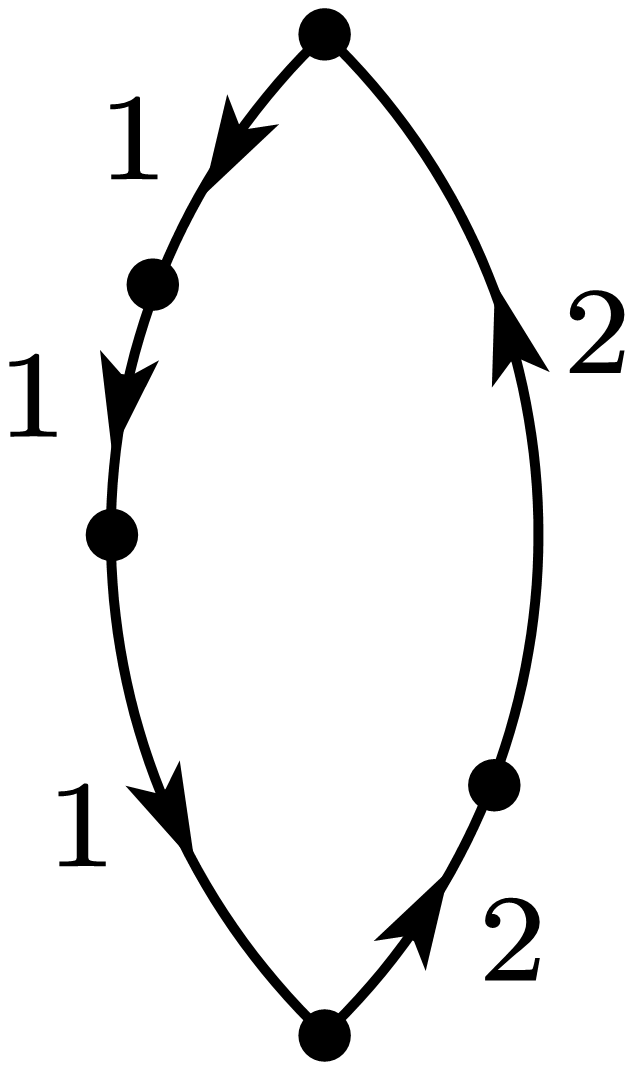
\includegraphics[scale=1.0,trim=0 -4 0 -4]{./pictures/6.01/2.png}
		\captionof*{figure}{$\displaystyle (-1)^{3+1} \frac{ V^2_{11} V_{12} V_{21} V_{22} }{ ( E^{(0)}_1 - E^{(0)}_2)^4 }$}
		\end{minipage} &
		
		\begin{minipage}{0.22\linewidth}
		\centering
		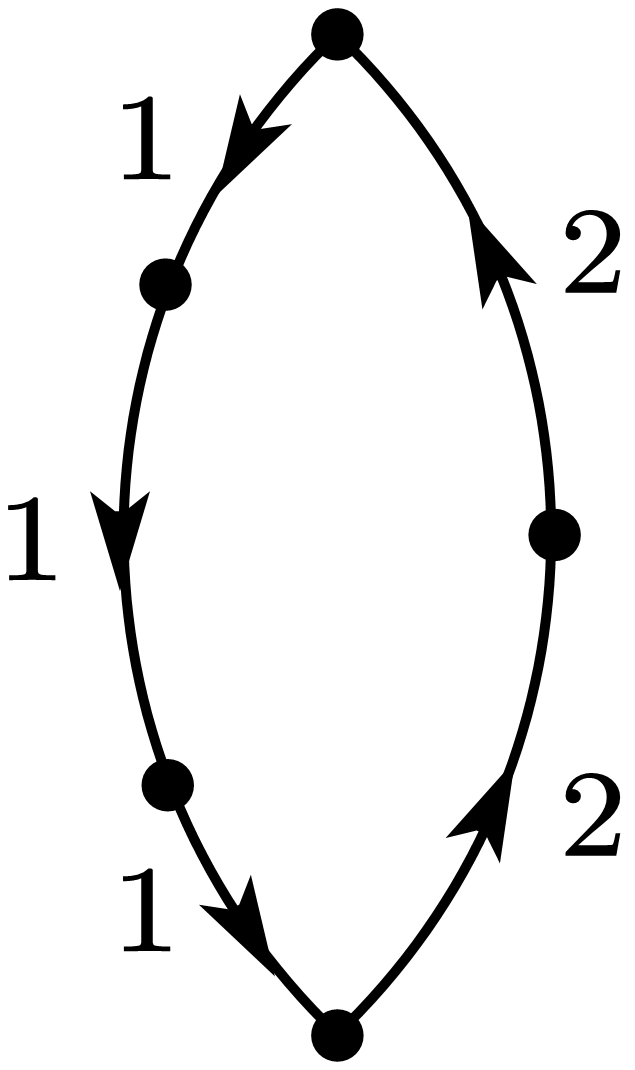
\includegraphics[scale=1.0,trim=0 -4 0 -4]{./pictures/6.01/3.png}
		\captionof*{figure}{$\displaystyle (-1)^{3+1} \frac{ V^2_{11} V_{12} V_{21} V_{22} }{ ( E^{(0)}_1 - E^{(0)}_2)^4 }$}
		\end{minipage} &
		
		\begin{minipage}{0.22\linewidth}
		\centering
		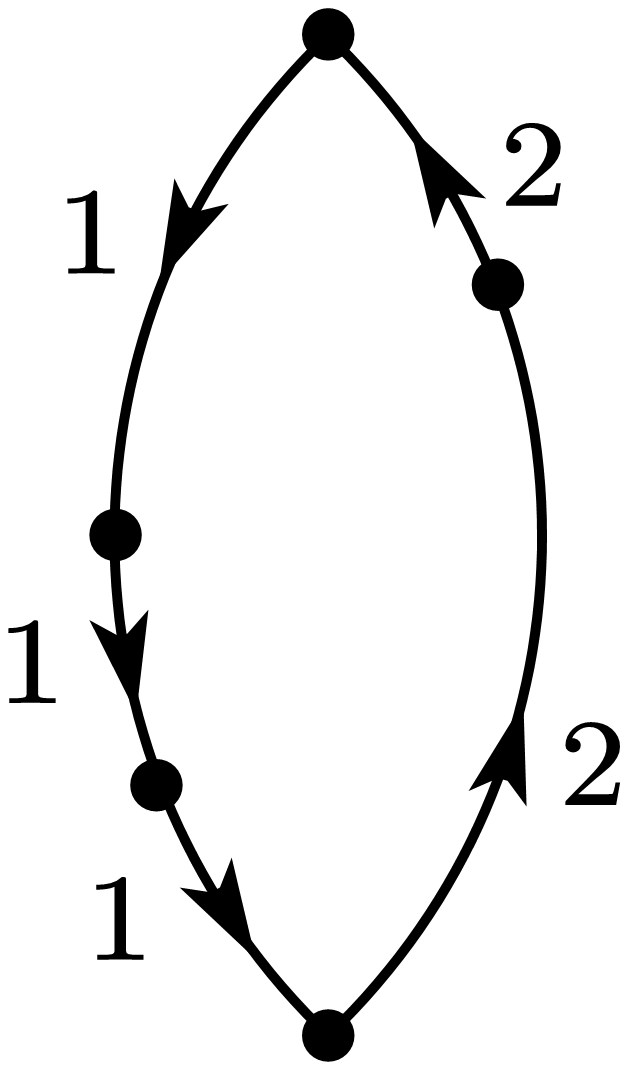
\includegraphics[scale=1.0,trim=0 -4 0 -4]{./pictures/6.01/4.png}
		\captionof*{figure}{$\displaystyle (-1)^{3+1} \frac{ V^2_{11} V_{12} V_{21} V_{22} }{ ( E^{(0)}_1 - E^{(0)}_2)^4 }$}
		\end{minipage} \\
			
		\begin{minipage}{0.22\linewidth}
		\centering
		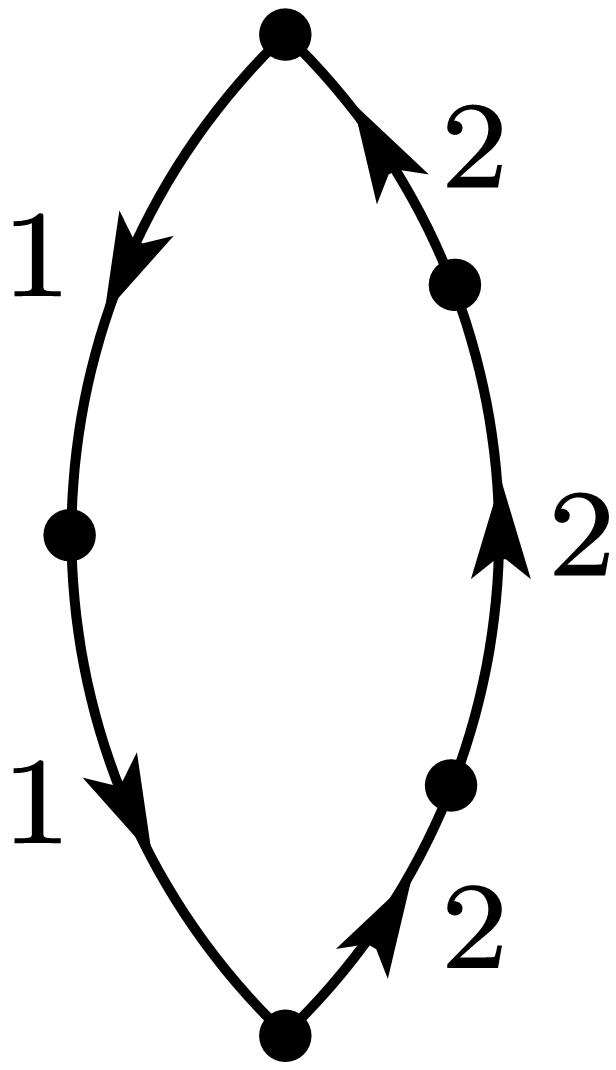
\includegraphics[scale=1.0,trim=0 -4 0 -4]{./pictures/6.01/5.png}
		\captionof*{figure}{$\displaystyle (-1)^{2+1} \frac{ V_{11} V_{12} V_{21} V^2_{22} }{ ( E^{(0)}_1 - E^{(0)}_2)^4 }$}
		\end{minipage} &
		
		\begin{minipage}{0.22\linewidth}
		\centering
		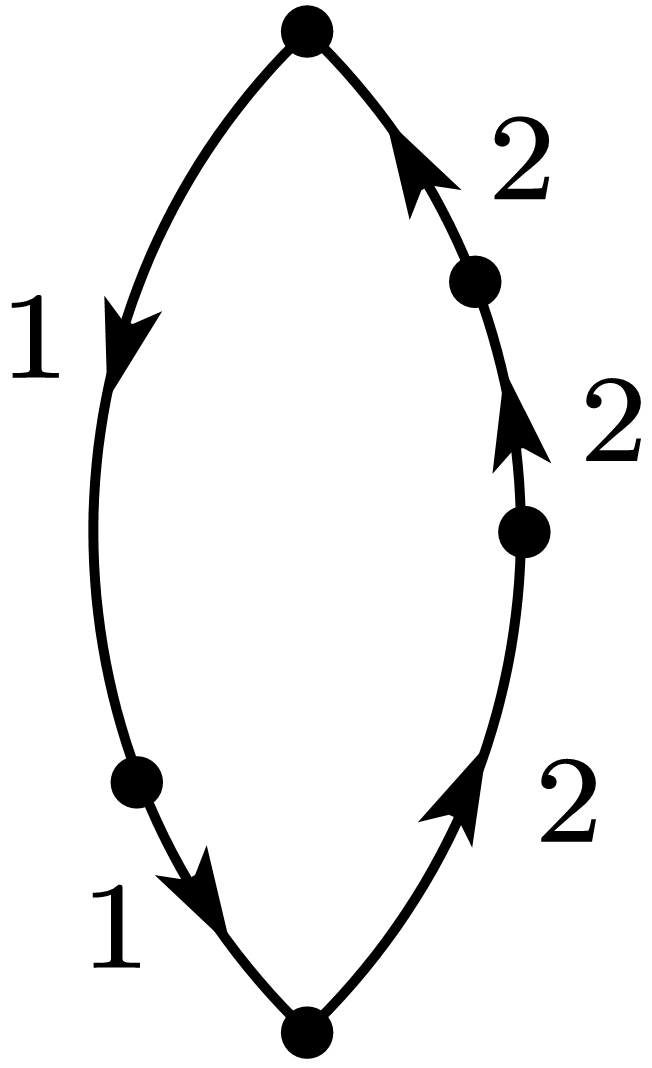
\includegraphics[scale=1.0,trim=0 -4 0 -4]{./pictures/6.01/6.png}
		\captionof*{figure}{$\displaystyle (-1)^{2+1} \frac{ V_{11} V_{12} V_{21} V^2_{22} }{ ( E^{(0)}_1 - E^{(0)}_2)^4 }$}
		\end{minipage} &
		
		\begin{minipage}{0.22\linewidth}
		\centering
		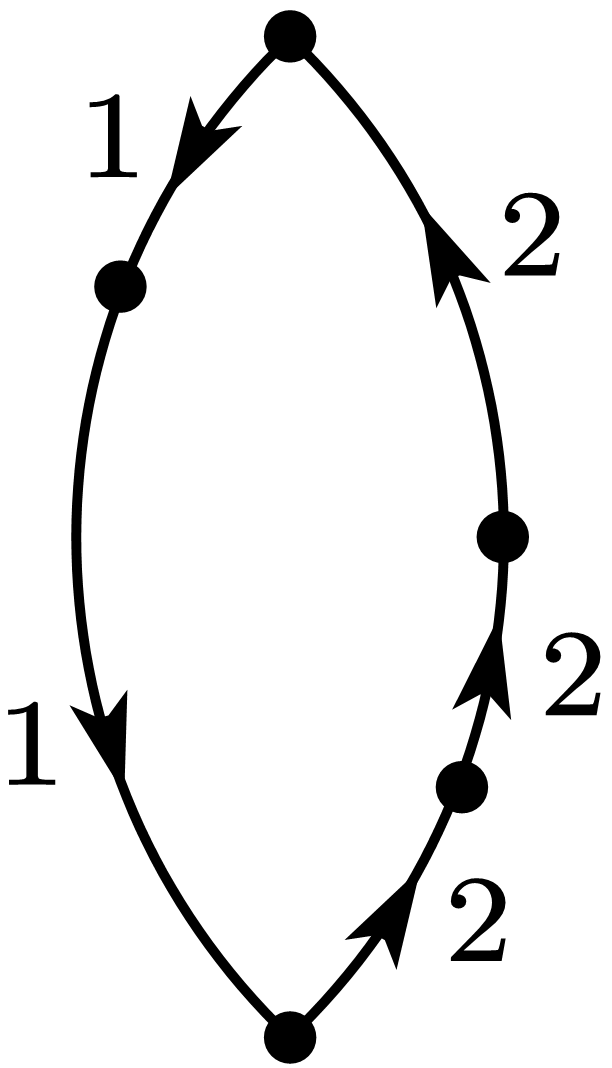
\includegraphics[scale=1.0,trim=0 -4 0 -4]{./pictures/6.01/7.png}
		\captionof*{figure}{$\displaystyle (-1)^{2+1} \frac{ V_{11} V_{12} V_{21} V^2_{22} }{ ( E^{(0)}_1 - E^{(0)}_2)^4 }$}
		\end{minipage} &
		
		\begin{minipage}{0.22\linewidth}
		\centering
		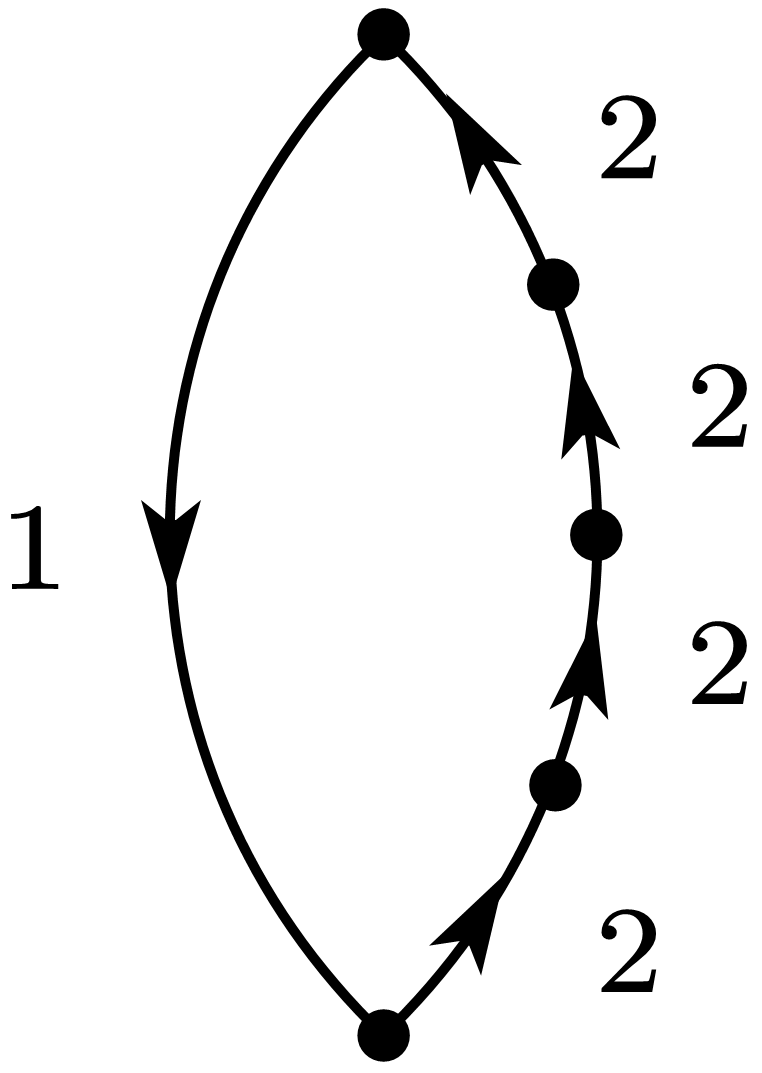
\includegraphics[scale=1.0,trim=0 -4 0 -4]{./pictures/6.01/8.png}
		\captionof*{figure}{$\displaystyle (-1)^{1+1} \frac{ V_{12} V_{21} V^3_{22} }{ ( E^{(0)}_1 - E^{(0)}_2)^4 }$}
		\end{minipage} 
		
	\end{tabular}
	\captionof{figure}{All fifth-order diagrams, which have the property that an imaginary horizontal line crosses only one hole and one particle line, and their mathematical expressions.}\label{fig:exe1}
	\end{center}
	
	Note that the diagrams, which have the property that an imaginary horizontal line crosses only one hole and one particle line, have no pair of hole/particle lines whose overlap is nonempty. For any pair of hole/particle lines which connect the dots $m_1$ and $n_1$, $m_2$ and $n_2$, where $n_1 > m_1$ and $n_2 > m_2$, their overlap will be 
	\begin{itemize}
	
	\item $[\max\{m_1, m_2\},\min\{n_1, n_2\}]$, if $\min\{n_1, n_2\} > \max\{m_1, m_2\}$;
	
	\item empty, otherwise. 
	
	\end{itemize}
	For example, if there is a pair of hole lines, one connecting the dot 1 and 3, and the other connecting 2 and 5, their overlap will be $[2, 3]$. Take an another example, if there is a pair of particle lines, one connecting the dot 5 and 4, and the other connecting 2 and 1, their overlap will be empty.
	
	Thus, there are four cases.
	\begin{itemize}
	
	\item Four hole lines and one particle line. There is only one method, hole lines are $(1,2)$, $(2,3)$, $(3,4)$, $(4,5)$ and the only particle line is $(5,1)$, as the first subdiagram in \Figref{fig:exe1}.
	
	\item Three hole lines and two particle lines. There are three methods as follows.
		\begin{itemize}
	
		\item Hole lines are $(1,2)$, $(2,3)$, and $(3,5)$ while particle lines are $(5,4)$, $(4,1)$.
		
		\item Hole lines are $(1,2)$, $(2,4)$, and $(4,5)$ while particle lines are $(5,3)$, $(3,1)$.
		
		\item Hole lines are $(1,3)$, $(3,4)$, and $(4,5)$ while particle lines are $(5,2)$, $(2,1)$.
	
		\end{itemize}
		They correspond to the second, third, fourth subdiagram in \Figref{fig:exe1}.
	
	\item Two hole lines and three particle lines. There are three methods as follows.
		\begin{itemize}
	
		\item Hole lines are $(1,3)$, $(3,5)$ while particle lines are $(5,4)$, $(4,2)$, and $(2,1)$.
		
		\item Hole lines are $(1,4)$, $(4,5)$ while particle lines are $(5,3)$, $(3,2)$, and $(2,1)$.
		
		\item Hole lines are $(1,2)$, $(2,5)$ while particle lines are $(5,4)$, $(4,3)$, and $(3,1)$.
	
		\end{itemize}
		They correspond to the fifth, sixth, seventh subdiagram in \Figref{fig:exe1}.
		
	\item One hole line and four particle lines. There is only one method, the only hole line is $(1,5)$ and particle lines are $(5,4)$, $(4,3)$, $(3,2)$, and $(2,1)$, as the eighth subdiagram in \Figref{fig:exe1}.
			
	\end{itemize}
	
	Thus, the sum of such diagrams is
	\begin{align*}
%		&\hspace{1.4em}(-1)^{4+1} \frac{ V^3_{11} V_{12} V_{21} }{ ( E^{(0)}_1 - E^{(0)}_2)^4 } + (-1)^{3+1} \frac{ V^2_{11} V_{12} V_{21} V_{22} }{ ( E^{(0)}_1 - E^{(0)}_2)^4 } + (-1)^{3+1} \frac{ V^2_{11} V_{12} V_{21} V_{22} }{ ( E^{(0)}_1 - E^{(0)}_2)^4 } \\
%		&\hspace{1.4em} + (-1)^{3+1} \frac{ V^2_{11} V_{12} V_{21} V_{22} }{ ( E^{(0)}_1 - E^{(0)}_2)^4 } + (-1)^{2+1} \frac{ V_{11} V_{12} V_{21} V^2_{22} }{ ( E^{(0)}_1 - E^{(0)}_2) }^4 + (-1)^{2+1} \frac{ V_{11} V_{12} V_{21} V^2_{22} }{ ( E^{(0)}_1 - E^{(0)}_2) }^4 \\
%		&\hspace{1.4em}  + (-1)^{2+1} \frac{ V_{11} V_{12} V_{21} V^2_{22} }{ ( E^{(0)}_1 - E^{(0)}_2) }^4 + (-1)^{1+1} \frac{ V_{12} V_{21} V^3_{22} }{ ( E^{(0)}_1 - E^{(0)}_2)^4 } \\
%		&= - \frac{ V^3_{11} V_{12} V_{21} }{ ( E^{(0)}_1 - E^{(0)}_2)^4 } + 3 \frac{ V^2_{11} V_{12} V_{21} V_{22} }{ ( E^{(0)}_1 - E^{(0)}_2)^4 } - 3 \frac{ V_{11} V_{12} V_{21} V^2_{22} }{ ( E^{(0)}_1 - E^{(0)}_2) }^4 + \frac{ V_{12} V_{21} V^3_{22} }{ ( E^{(0)}_1 - E^{(0)}_2)^4 } \\
%		&= 
		- \frac{ V_{12} V_{21} \left( V^3_{11} - 3 V^2_{11} V_{22} + 3 V_{11} V_{22} - V^3_{22} \right) }{ ( E^{(0)}_1 - E^{(0)}_2)^4 } = - \frac{ V_{12} V_{21} \left( V_{11} - V_{22} \right)^3 }{ ( E^{(0)}_1 - E^{(0)}_2)^4 } = \frac{ V_{12} V_{21} \left( V_{22} - V_{11} \right)^3 }{ ( E^{(0)}_1 - E^{(0)}_2)^4 }.
	\end{align*}
	
	In fact, as the textbook says, these eight diagrams can be generated by adding three dots to the second-order diagram in all positive ways. In fact, any pair of hole/particle lines in them has also empty overlap. I think the calculation of the overlap is much direct than inspecting the property of lines.
	
	\end{solution}

	\subsection{Diagrammatic Perturbation Theory for \texorpdfstring{$N$}- States}
	
	% 6.2
	\begin{exercise}
	Use diagrammatic techniques to obtain the fourth-order perturbation energy of a particular state (say, $i$) of an $N$-state system. That is, evaluate the diagrams
	\begin{center}
	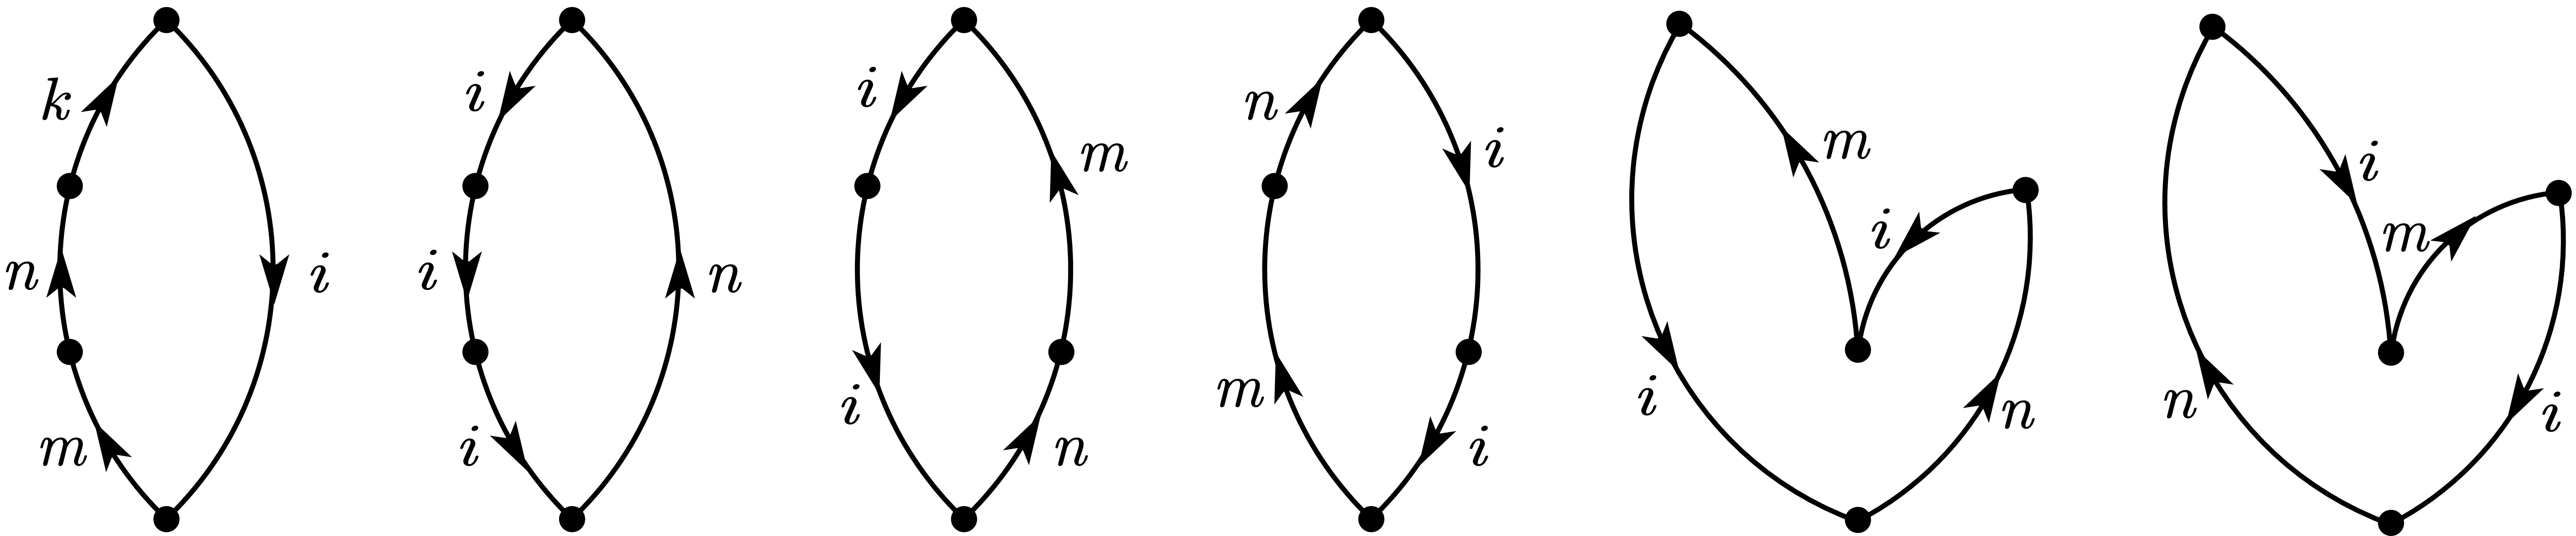
\includegraphics[scale=1.0]{./pictures/6.02/exercise.png}
	\end{center}
	where the indices $m$, $n$, $k$, ... exclude $i$. Using the approach of Section 6.1, obtain an algebraic expression for the fourth-order energy and compare it to the diagrammatic result.
	
	\end{exercise}
	
	\begin{solution}
	
	Firstly, all fourth-order diagrams and their mathematical expressions are listed in \Figref{fig:exe2}.
	
	\begin{center}
	\begin{tabular}{cc}
	
		\begin{minipage}{0.49\linewidth}
		\centering
		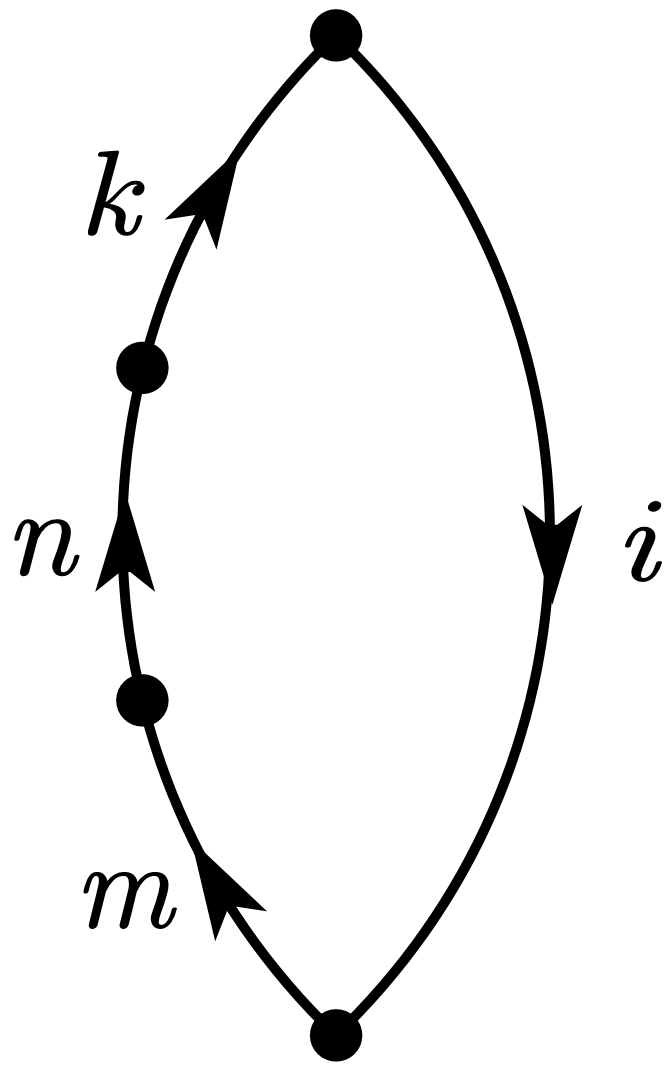
\includegraphics[scale=1.0,trim=0 -4 0 -4]{./pictures/6.02/1.png}
		\captionof*{figure}{$(-1)^{1+1} { \sum_{kmn} }^\prime \frac{ V_{ki} V_{nk} V_{mn} V_{im} }{ ( E^{(0)}_i - E^{(0)}_k ) ( E^{(0)}_i - E^{(0)}_n ) ( E^{(0)}_i - E^{(0)}_m ) }$}
		\end{minipage} &
		
		\begin{minipage}{0.42\linewidth}
		\centering
		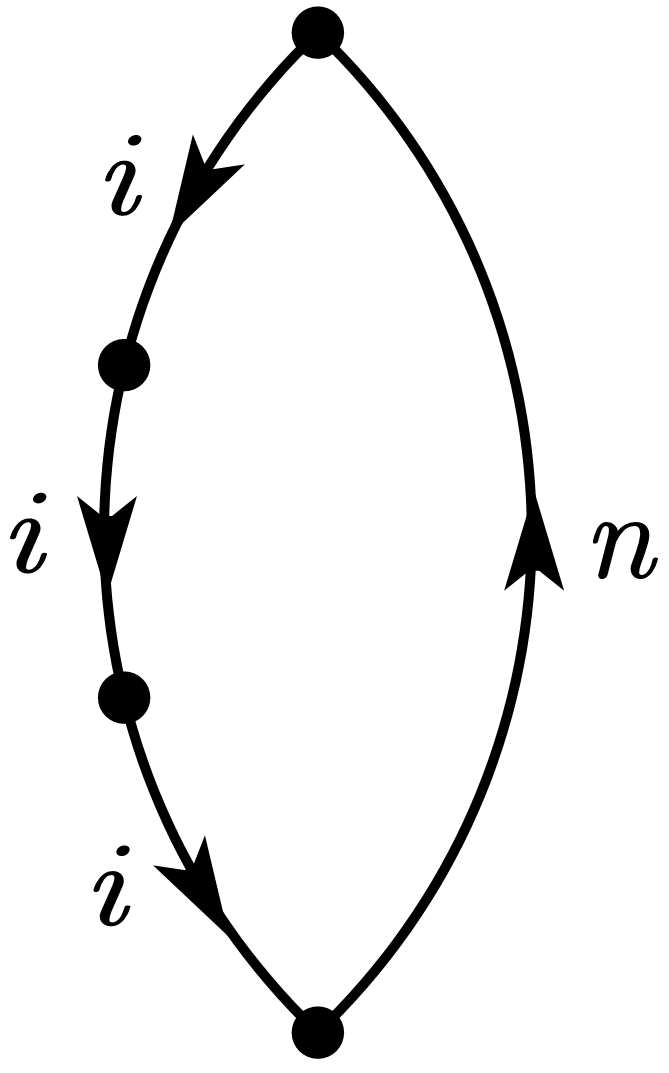
\includegraphics[scale=1.0,trim=0 -4 0 -4]{./pictures/6.02/2.png}
		\captionof*{figure}{$(-1)^{3+1} { \sum_n }^\prime \frac{ V_{ni} V^2_{ii} V_{in} }{ ( E^{(0)}_i - E^{(0)}_n)^3 }$}
		\end{minipage} \\
		
		\begin{minipage}{0.49\linewidth}
		\centering
		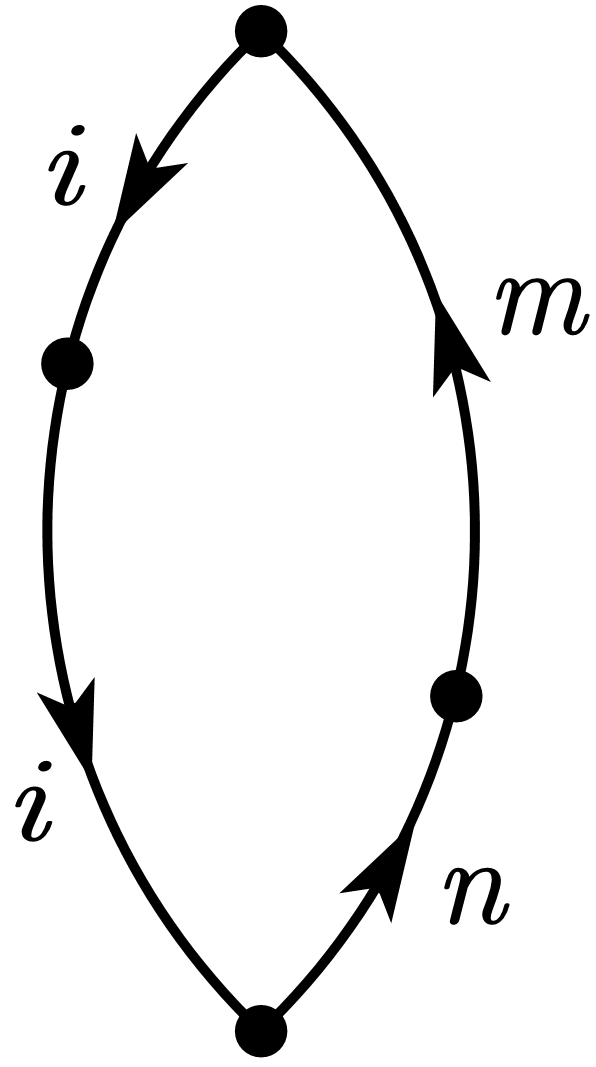
\includegraphics[scale=1.0,trim=0 -4 0 -4]{./pictures/6.02/3.png}
		\captionof*{figure}{$(-1)^{2+1} { \sum_{mn} }^\prime \frac{ V_{mi} V_{ii} V_{in} V_{nm} }{ ( E^{(0)}_i - E^{(0)}_n) ( E^{(0)}_i - E^{(0)}_m )^2 }$}
		\end{minipage}  &
			
		\begin{minipage}{0.42\linewidth}
		\centering
		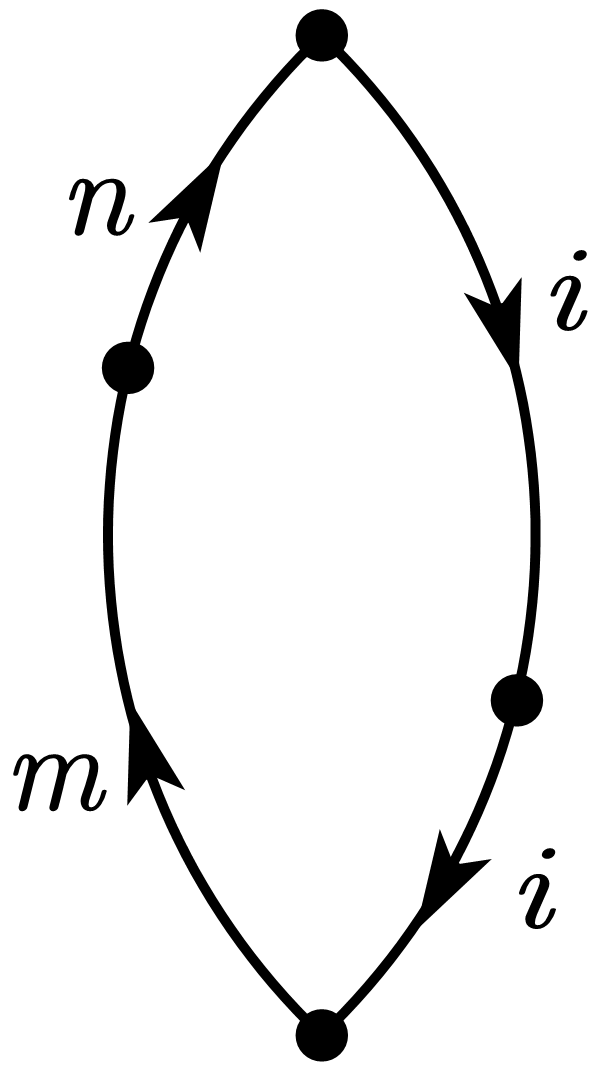
\includegraphics[scale=1.0,trim=0 -4 0 -4]{./pictures/6.02/4.png}
		\captionof*{figure}{$(-1)^{2+1} { \sum_{mn} }^\prime \frac{ V_{ni} V_{ii} V_{im} V_{mn} }{ ( E^{(0)}_i - E^{(0)}_n) ( E^{(0)}_i - E^{(0)}_m )^2 }$}
		\end{minipage} \\
		
		\begin{minipage}{0.49\linewidth}
		\centering
		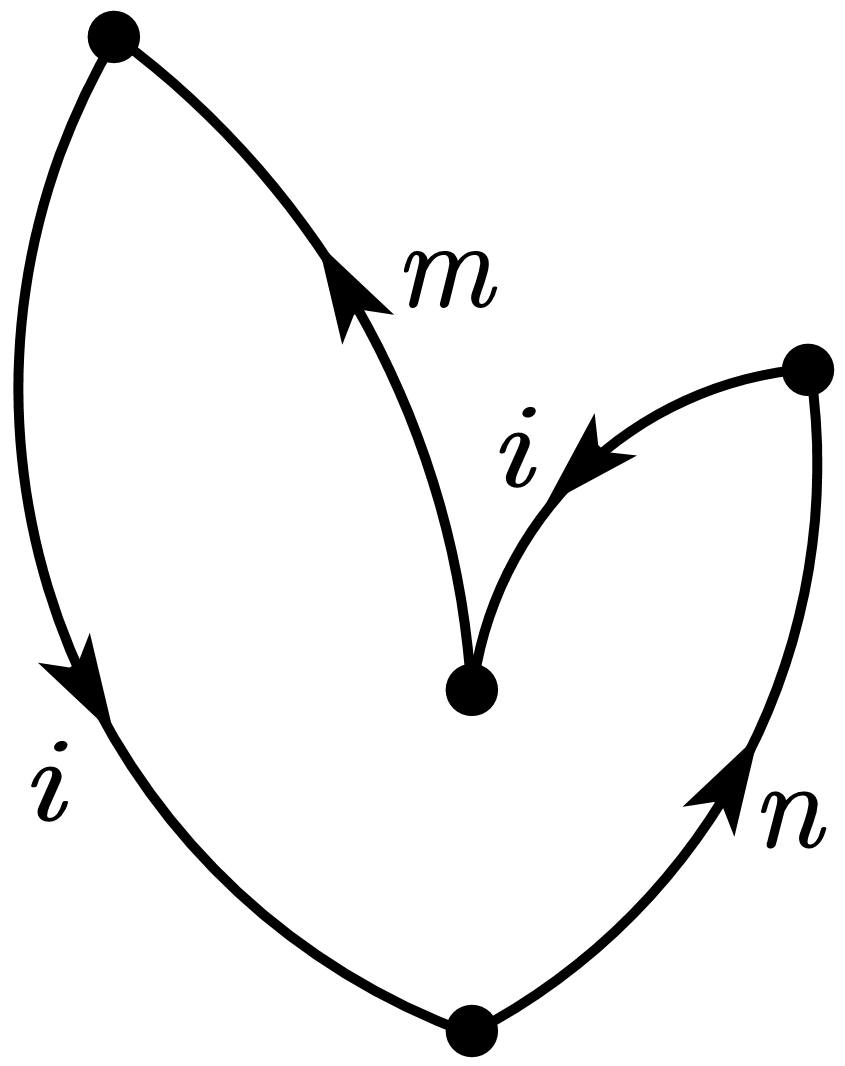
\includegraphics[scale=1.0,trim=0 -4 0 -4]{./pictures/6.02/5.png}
		\captionof*{figure}{$(-1)^{2+1} { \sum_{mn} }^\prime \frac{ V_{mi} V_{in} V_{ni} V_{im} }{ ( E^{(0)}_i - E^{(0)}_m ) ( 2E^{(0)}_i - E^{(0)}_m - E^{(0)}_n ) ( E^{(0)}_i - E^{(0)}_n ) }$}
		\end{minipage} &
		
		\begin{minipage}{0.42\linewidth}
		\centering
		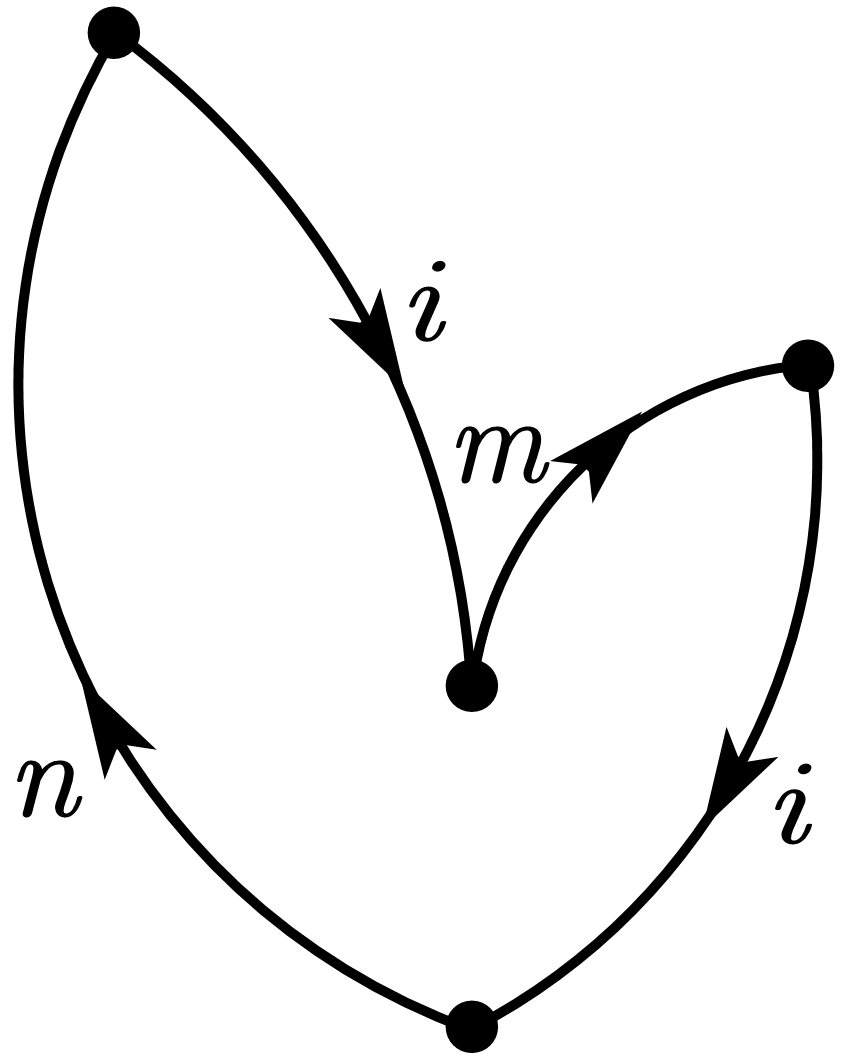
\includegraphics[scale=1.0,trim=0 -4 0 -4]{./pictures/6.02/6.png}
		\captionof*{figure}{$(-1)^{2+1} { \sum_{mn} }^\prime \frac{ V_{in} V_{ni} V_{im} V_{mi} }{ ( 2E^{(0)}_i - E^{(0)}_m - E^{(0)}_n ) ( E^{(0)}_i - E^{(0)}_n )^2 }$}
		\end{minipage} 
				
	\end{tabular}
	\captionof{figure}{All fourth-order diagrams and their mathematical expressions.}\label{fig:exe2}
	\end{center}
	
	Before the formal algebraic derivation, we should obtain some useful intermediate results. From (6.7d), multiplying by $\langle n |$, where $n \neq i$, we find that
	\[
		E^{(0)}_n \langle n | \Psi^{(3)}_i \rangle + \langle n | \mathscr{V} | \Psi^{(2)}_i \rangle = E^{(0)}_i \langle n | \Psi^{(3)}_i \rangle + E^{(1)}_i \langle n | \Psi^{(2)}_i \rangle + E^{(1)}_i \langle n | \Psi^{(2)}_i \rangle,
	\]
	and thus
	\[
		\langle n | \Psi^{(3)}_i \rangle = \frac{ 1 }{ E^{(0)}_i - E^{(0)}_n }\left[ \langle n | \mathscr{V} | \Psi^{(2)}_i \rangle - E^{(1)}_i \langle n | \Psi^{(2)}_i \rangle - E^{(1)}_i \langle n | \Psi^{(2)}_i \rangle \right].
	\]
	Moreover, (6.8b), (6.10), (6.12), and (6.14) are used in the formal derivation. The fourth-order perturbation energy $E^{(4)}_i$ can be divided into 3 terms, viz.,
	\begin{align*}
		E^{(4)}_i &= \langle i | \mathscr{V} | \Psi^{(3)}_i \rangle = { \sum_n }^\prime \langle i | \mathscr{V} | n \rangle \langle n | \Psi^{(3)}_i \rangle = { \sum_n }^\prime V_{in} \frac{ \langle n | \mathscr{V} | \Psi^{(2)}_i \rangle - E^{(1)}_i \langle n | \Psi^{(2)}_i \rangle - E^{(2)}_i \langle n | \Psi^{(1)}_i \rangle }{ E^{(0)}_i - E^{(0)}_n } \\
		&= { \sum_n }^\prime \frac{ V_{in} \langle n | \mathscr{V} | \Psi^{(2)}_i \rangle }{ E^{(0)}_i - E^{(0)}_n } - E^{(1)}_i { \sum_n }^\prime \frac{ V_{in} \langle n | \Psi^{(2)}_i \rangle }{ E^{(0)}_i - E^{(0)}_n } - E^{(2)}_i { \sum_n }^\prime \frac{ V_{in} \langle n | \Psi^{(1)}_i \rangle }{ E^{(0)}_i - E^{(0)}_n }.
	\end{align*}		
	The first term is
	\begin{align*}
		&\hspace{1.4em}{ \sum_n }^\prime \frac{ V_{in} \langle n | \mathscr{V} | \Psi^{(2)}_i \rangle }{ E^{(0)}_i - E^{(0)}_n } = { \sum_{mn} }^\prime \frac{ V_{in} \langle n | \mathscr{V} | m \rangle \langle m | \Psi^{(2)}_i \rangle }{ E^{(0)}_i - E^{(0)}_n } = { \sum_{mn} }^\prime \frac{ V_{in} V_{nm} }{ E^{(0)}_i - E^{(0)}_n } \langle m | \Psi^{(2)}_i \rangle \\
		&= { \sum_{mn} }^\prime \frac{ V_{in} V_{nm} }{ E^{(0)}_i - E^{(0)}_n } \frac{ \langle m | \mathscr{V} | \Psi^{(1)}_i \rangle - E^{(1)}_i \langle m | \Psi^{(1)}_i \rangle }{ E^{(0)}_i - E^{(0)}_m } \\
		&= { \sum_{mn} }^\prime \frac{ V_{in} V_{nm} }{ ( E^{(0)}_i - E^{(0)}_n )( E^{(0)}_i - E^{(0)}_m ) } \left[ \langle m | \mathscr{V} | \Psi^{(1)}_i \rangle - E^{(1)}_i \langle m | \Psi^{(1)}_i \rangle \right] \\
		&= { \sum_{mn} }^\prime \frac{ V_{in} V_{nm} }{ (E^{(0)}_i - E^{(0)}_n) (E^{(0)}_i - E^{(0)}_m) } \left[ { \sum_k }^\prime \langle m | \mathscr{V} | k \rangle \langle k | \Psi^{(1)}_i \rangle - E^{(1)}_i \langle m | \Psi^{(1)}_i \rangle \right] \\
		&= { \sum_{mnk} }^\prime \frac{ V_{in} V_{nm} V_{mk} }{ (E^{(0)}_i - E^{(0)}_n) (E^{(0)}_i - E^{(0)}_m) } \langle k | \Psi^{(1)}_i \rangle - { \sum_{mn} }^\prime \frac{ V_{ii} V_{in} V_{nm} }{ (E^{(0)}_i - E^{(0)}_n) (E^{(0)}_i - E^{(0)}_m) } \langle m | \Psi^{(1)}_i \rangle \\
		&= { \sum_{mnk} }^\prime \frac{ V_{in} V_{nm} V_{mk} }{ (E^{(0)}_i - E^{(0)}_n) (E^{(0)}_i - E^{(0)}_m) } \frac{ V_{ki} }{ E^{(0)}_i - E^{(0)}_k } - { \sum_{mn} }^\prime \frac{ V_{ii} V_{in} V_{nm} }{ (E^{(0)}_i - E^{(0)}_n) (E^{(0)}_i - E^{(0)}_m) } \frac{ V_{mi} }{ E^{(0)}_i - E^{(0)}_m } \\
		&= { \sum_{mnk} }^\prime \frac{ V_{in} V_{nm} V_{mk} V_{ki} }{ (E^{(0)}_i - E^{(0)}_n) (E^{(0)}_i - E^{(0)}_m) (E^{(0)}_i - E^{(0)}_k) } - { \sum_{mn} }^\prime \frac{ V_{ii} V_{in} V_{nm} V_{mi} }{ (E^{(0)}_i - E^{(0)}_n) (E^{(0)}_i - E^{(0)}_m)^2 } \\
		&= { \sum_{mnk} }^\prime \frac{ V_{im} V_{mn} V_{nk} V_{ki} }{ (E^{(0)}_i - E^{(0)}_n) (E^{(0)}_i - E^{(0)}_m) (E^{(0)}_i - E^{(0)}_k) } - { \sum_{mn} }^\prime \frac{ V_{ii} V_{in} V_{nm} V_{mi} }{ (E^{(0)}_i - E^{(0)}_n) (E^{(0)}_i - E^{(0)}_m)^2 }.
	\end{align*}
	It is evident that the first part of the first term correspond to the first subdiagram and the second part of the first term correspond to the third subdiagram.
	
	The second term is
	\begin{align*}
		&\hspace{1.4em}- E^{(1)}_i { \sum_n }^\prime \frac{ V_{in} \langle n | \Psi^{(2)}_i \rangle }{ E^{(0)}_i - E^{(0)}_n } - { \sum_n }^\prime \frac{ V_{ii} V_{in} }{ E^{(0)}_i - E^{(0)}_n } \langle n | \Psi^{(2)}_i \rangle \\
		&= - { \sum_n }^\prime \frac{ V_{ii} V_{in} }{ E^{(0)}_i - E^{(0)}_n } \frac{ \langle n | \mathscr{V} | \Psi^{(1)}_i \rangle - E^{(1)}_i \langle n | \Psi^{(1)}_i \rangle }{ E^{(0)}_i - E^{(0)}_n } \\
		&= - { \sum_n }^\prime \frac{ V_{ii} V_{in} }{ ( E^{(0)}_i - E^{(0)}_n )^2 } \langle n | \mathscr{V} | \Psi^{(1)}_i \rangle + E^{(1)}_i { \sum_n }^\prime \frac{ V_{ii} V_{in} }{ ( E^{(0)}_i - E^{(0)}_n )^2 } \langle n | \Psi^{(1)}_i \rangle \\
		&= - { \sum_n }^\prime \frac{ V_{ii} V_{in} }{ ( E^{(0)}_i - E^{(0)}_n )^2 } { \sum_m }^\prime \langle n | \mathscr{V} | m \rangle \langle m | \Psi^{(1)}_i \rangle + { \sum_n }^\prime \frac{ V^2_{ii} V_{in} }{ ( E^{(0)}_i - E^{(0)}_n )^2 } \langle n | \Psi^{(1)}_i \rangle \\
		&= - { \sum_{mn} }^\prime \frac{ V_{ii} V_{in} V_{nm} }{ ( E^{(0)}_i - E^{(0)}_n )^2 } \langle m | \Psi^{(1)}_i \rangle + { \sum_n }^\prime \frac{ V^2_{ii} V_{in} }{ ( E^{(0)}_i - E^{(0)}_n )^2 } \langle n | \Psi^{(1)}_i \rangle \\
		&= - { \sum_{mn} }^\prime \frac{ V_{ii} V_{in} V_{nm} }{ ( E^{(0)}_i - E^{(0)}_n )^2 } \frac{ \langle m | \mathscr{V} | i \rangle }{ E^{(0)}_i - E^{(0)}_m } + { \sum_n }^\prime \frac{ V^2_{ii} V_{in} }{ ( E^{(0)}_i - E^{(0)}_n )^2 } \frac{ \langle n | \mathscr{V} | i \rangle }{ E^{(0)}_i - E^{(0)}_n } \\
		&= - { \sum_{mn} }^\prime \frac{ V_{ii} V_{in} V_{nm} V_{mi} }{ ( E^{(0)}_i - E^{(0)}_n )^2 (E^{(0)}_i - E^{(0)}_m) } + { \sum_n }^\prime \frac{ V^2_{ii} V_{in} V_{ni} }{ ( E^{(0)}_i - E^{(0)}_n )^3 } \\
		&= - { \sum_{mn} }^\prime \frac{ V_{ii} V_{im} V_{mn} V_{ni} }{ ( E^{(0)}_i - E^{(0)}_m )^2 ( E^{(0)}_i - E^{(0)}_n ) } + { \sum_n }^\prime \frac{ V^2_{ii} V_{in} V_{ni} }{ ( E^{(0)}_i - E^{(0)}_n )^3 } .
	\end{align*}
	It is evident that the first part of the second term correspond to the fourth subdiagram and the second part of the second term correspond to the second subdiagram.
	
	The third term is
	\begin{align*}
		&\hspace{1.4em} -E^{(2)}_i { \sum_n }^\prime \frac{ V_{in} \langle n | \Psi^{(1)}_i \rangle }{ E^{(0)}_i - E^{(0)}_n } = -E^{(2)}_i { \sum_n }^\prime \frac{ V_{in} }{ E^{(0)}_i - E^{(0)}_n } \frac{ \langle n | \mathscr{V} | i \rangle }{ E^{(0)}_i - E^{(0)}_n } = -E^{(2)}_i { \sum_n }^\prime \frac{ V_{in} V_{ni} }{ ( E^{(0)}_i - E^{(0)}_n )^2 } \\
		&= - \left( { \sum_m }^\prime \frac{ V_{im} V_{mi} }{ ( E^{(0)}_i - E^{(0)}_m ) } \right) { \sum_n }^\prime \frac{ V_{in} V_{ni} }{ ( E^{(0)}_i - E^{(0)}_n )^2 } = - { \sum_{mn} }^\prime \frac{ V_{im} V_{mi} V_{in} V_{ni} }{ ( E^{(0)}_i - E^{(0)}_m )( E^{(0)}_i - E^{(0)}_n )^2 } .
	\end{align*}		
	
	It seems that it does not directly correspond to any subdiagram in \Figref{fig:exe2}. However, we can find that the sum of the mathematical expressions of the fifth and sixth subdiagram is
	\begin{align*}
		&\hspace{1.4em}(-1)^{2+1} { \sum_{mn} }^\prime \frac{ V_{mi} V_{in} V_{ni} V_{im} }{ ( E^{(0)}_i - E^{(0)}_m ) ( 2E^{(0)}_i - E^{(0)}_m - E^{(0)}_n ) ( E^{(0)}_i - E^{(0)}_n ) }  \\
		&\hspace{3.4em}+ (-1)^{2+1} { \sum_{mn} }^\prime \frac{ V_{in} V_{ni} V_{im} V_{mi} }{ ( 2E^{(0)}_i - E^{(0)}_m - E^{(0)}_n ) ( E^{(0)}_i - E^{(0)}_n )^2 } \\
		&= - { \sum_{mn} }^\prime \frac{ V_{in} V_{ni} V_{im} V_{mi} }{ ( 2E^{(0)}_i - E^{(0)}_m - E^{(0)}_n ) ( E^{(0)}_i - E^{(0)}_n ) } \left[ \frac{ 1 }{ E^{(0)}_i - E^{(0)}_m } + \frac{ 1 }{ E^{(0)}_i - E^{(0)}_n } \right] \\
		&= - { \sum_{mn} }^\prime \frac{ V_{in} V_{ni} V_{im} V_{mi} }{ ( 2E^{(0)}_i - E^{(0)}_m - E^{(0)}_n ) ( E^{(0)}_i - E^{(0)}_n ) } \frac{ 2E^{(0)}_i - E^{(0)}_m - E^{(0)}_n }{ ( E^{(0)}_i - E^{(0)}_m )( E^{(0)}_i - E^{(0)}_n ) } \\
		&= - { \sum_{mn} }^\prime \frac{ V_{im} V_{mi} V_{in} V_{ni} }{ ( E^{(0)}_i - E^{(0)}_m )( E^{(0)}_i - E^{(0)}_n )^2 } ,
	\end{align*}
	which is the third term exactly. Thus we can conclude that the results obtained by algebraic methods is the same as that by diagrammatic techniques. The mathematical expression of the fourth-order perturbation energy $E^{(4)}_i$ is
	\begin{align*}
		E^{(4)}_i &= { \sum_{mnk} }^\prime \frac{ V_{im} V_{mn} V_{nk} V_{ki} }{ (E^{(0)}_i - E^{(0)}_n) (E^{(0)}_i - E^{(0)}_m) (E^{(0)}_i - E^{(0)}_k) } - { \sum_{mn} }^\prime \frac{ V_{ii} V_{in} V_{nm} V_{mi} }{ (E^{(0)}_i - E^{(0)}_n) (E^{(0)}_i - E^{(0)}_m)^2 } \\
		&\hspace{2em} - { \sum_{mn} }^\prime \frac{ V_{ii} V_{im} V_{mn} V_{ni} }{ ( E^{(0)}_i - E^{(0)}_m )^2 ( E^{(0)}_i - E^{(0)}_n ) } + { \sum_n }^\prime \frac{ V^2_{ii} V_{in} V_{ni} }{ ( E^{(0)}_i - E^{(0)}_n )^3 } - { \sum_{mn} }^\prime \frac{ V_{im} V_{mi} V_{in} V_{ni} }{ ( E^{(0)}_i - E^{(0)}_m )( E^{(0)}_i - E^{(0)}_n )^2 } .
	\end{align*}
	
	\end{solution}
	
	\subsection{Summation of Diagrams}
	
	\section{Orbital Perturbation Theory: One-Particle Perturbations}	
	
	% 6.3	
	\begin{exercise}
	Derive
	\[
		E^{(2)}_0 = \sum_{ar} \frac{v_{ar}v_{ra}}{\varepsilon^{(0)}_a - \varepsilon^{(0)}_r}
	\]
	starting with the general expression for the second-order energy (Eq.(6.12)) applied to an $N$-electron system,
	\[
		E^{(2)}_0 = { \sum_n }^\prime \frac{\left| \langle \Psi_0 | \displaystyle\sum_i v(i)| n \rangle \right|^2 }{E^{(0)}_0-E^{(0)}_n}
	\]
	where the sum runs over all states of the system except the ground state.
	
	{\it Hint}: The states $| n \rangle$ must be single excitations of the type
	\[
		|\Psi^r_a\rangle = | \chi^{(0)}_1 \cdots \chi^{(0)}_{a-1} \chi^{(0)}_{r} \chi^{(0)}_{a+1} \cdots \chi^{(0)}_{N} \rangle.
	\]
	\end{exercise}
	
	\begin{solution}
	
	Note that (6.31) states that $\mathscr{V}=\sum_i v(i)$ only connects two Slater determinants whose different occupied orbitals should be no more than one, thus we obtain that
	\begin{sequation}
		E^{(2)}_0 = { \sum_n }^\prime \frac{\left| \langle \Psi_0 | \sum_i v(i)| n \rangle \right|^2 }{E^{(0)}_0-E^{(0)}_n} = \sum_{ ar } \frac{ \left| \langle \Psi_0 | \mathscr{V} | \Psi^r_a \rangle \right|^2 }{E^{(0)}_0-(E^{(0)}_0 + \varepsilon^{(0)}_r - \varepsilon^{(0)}_a) } = \sum_{ ar } \frac{ v_{ar} v_{ra} }{ \varepsilon^{(0)}_a - \varepsilon^{(0)}_r }.
	\end{sequation}
	
	\end{solution}
	
	% 6.4
	\begin{exercise}
	Calculate the third-order energy $E^{(3)}_0$ using the general expression given in Eq.(6.15).
	\begin{enumerate}
	
	\item[a.] Show that
	\[
		B^{(3)}_0 = - E^{(1)}_0 { \sum_n }^\prime \frac{|\langle \Psi_0 | \mathscr{V} | n \rangle |^2}{(E^{(0)}_0-E^{(0)}_n)^2} = - \sum_{abr} \frac{v_{aa} v_{rb} v_{br}}{( \varepsilon^{(0)}_b - \varepsilon^{(0)}_r)^2}.
	\]
		
	\item[b.] Show that
	\[
		A^{(3)}_0 = { \sum_{nm} }^\prime \frac{\langle \Psi_0 | \mathscr{V} | n \rangle \langle n | \mathscr{V} | m \rangle \langle m | \mathscr{V} | \Psi_0 \rangle}{(E^{(0)}_0-E^{(0)}_n)(E^{(0)}_0-E^{(0)}_m)} = \sum_{abrs} \frac{v_{ar} v_{sb} \langle \Psi^r_a | \mathscr{V} | \Psi^s_b \rangle}{( \varepsilon^{(0)}_a - \varepsilon^{(0)}_r)( \varepsilon^{(0)}_b - \varepsilon^{(0)}_s)}.
	\]
	
	\item[c.] Show that
	\begin{align*}
		\langle \Psi^r_a | \mathscr{V} | \Psi^s_b \rangle &= v_{rs} & \text{if} \, a = b  \quad r \neq s, \\
		&= - v_{ba} & \text{if} \, a \neq b \quad r = s, \\
		&= \sum_{c} v_{cc} - v_{aa} + v_{rr} & \text{if} \, a = b \quad r = s ,
	\end{align*}
	and zero otherwise.
		
	\item[d.] Finally, combine the two terms to obtain
	\[
		E^{(3)}_0 = A^{(3)}_0 + B^{(3)}_0 = \sum_{ars} \frac{v_{ar} v_{rs} v_{sa}}{( \varepsilon^{(0)}_a - \varepsilon^{(0)}_r)( \varepsilon^{(0)}_a - \varepsilon^{(0)}_s)} - \sum_{abr} \frac{v_{ra} v_{ab} v_{br}}{( \varepsilon^{(0)}_a - \varepsilon^{(0)}_r) ( \varepsilon^{(0)}_b - \varepsilon^{(0)}_r)}.
	\]
	
	\item[e.] Show that for a chosed-shell system
	\[
		E^{(3)}_0 = 2\sum_{ars}^{N/2} \frac{v_{ar} v_{rs} v_{sa}}{( \varepsilon^{(0)}_a - \varepsilon^{(0)}_r)( \varepsilon^{(0)}_a - \varepsilon^{(0)}_s)} - 2\sum_{abr}^{N/2} \frac{v_{ra} v_{ab} v_{br}}{( \varepsilon^{(0)}_a - \varepsilon^{(0)}_r) ( \varepsilon^{(0)}_b - \varepsilon^{(0)}_r)}.
	\]
	
	\end{enumerate}
	\end{exercise}
	
	\begin{solution}
	
	\begin{itemize}
	
	\item[a.] Similar to Exercise 6.3, it is evident that
	\begin{align*}
		B^{(3)}_0 &= - E^{(1)}_0 { \sum_n }^\prime \frac{|\langle \Psi_0 | \mathscr{V} | n \rangle |^2}{(E^{(0)}_0-E^{(0)}_n)^2} = - \left( \sum_{a} v_{aa} \right) \sum_{br} \frac{ v_{rb} v_{br}}{[ E^{(0)}_0- ( E^{(0)}_n + \varepsilon^{(0)}_r - \varepsilon^{(0)}_b ) ]^2} \\
		&= - \sum_{abr} \frac{ v_{aa} v_{rb} v_{br}}{( \varepsilon^{(0)}_b - \varepsilon^{(0)}_r)^2}.
	\end{align*}

	\item[b.] In the same way, we obtain that
	\begin{align*}
		A^{(3)}_0 &= { \sum_{nm} }^\prime \frac{\langle \Psi_0 | \mathscr{V} | n \rangle \langle n | \mathscr{V} | m \rangle \langle m | \mathscr{V} | \Psi_0 \rangle}{(E^{(0)}_0-E^{(0)}_n)(E^{(0)}_0-E^{(0)}_m)} \\
		&= \sum_{ar} \sum_{bs} \frac{\langle \Psi_0 | \mathscr{V} | \Psi^r_a \rangle \langle \Psi^r_a | \mathscr{V} | \Psi^s_b \rangle \langle \Psi^s_b | \mathscr{V} | \Psi_0 \rangle}{ [ E^{(0)}_0 - ( E^{(0)}_0 + \varepsilon^{(0)}_r - \varepsilon^{(0)}_a ) ][ E^{(0)}_0 - ( E^{(0)}_0 + \varepsilon^{(0)}_s - \varepsilon^{(0)}_b ) ]}  \\
		&= \sum_{abrs} \frac{v_{ar} v_{sb} \langle \Psi^r_a | \mathscr{V} | \Psi^s_b \rangle}{( \varepsilon^{(0)}_a - \varepsilon^{(0)}_r)( \varepsilon^{(0)}_b - \varepsilon^{(0)}_s)}.
	\end{align*}
	
	\item[c.] Using the conclusion of Exercise 2.13, at once we get
	\begin{align*}
		\langle \Psi^r_a | \mathscr{V} | \Psi^s_b \rangle &= v_{rs} & \text{if} \, a = b  \quad r \neq s, \\
		&= - v_{ba} & \text{if} \, a \neq b \quad r = s, \\
		&= \sum_{c} v_{cc} - v_{aa} + v_{rr} & \text{if} \, a = b \quad r = s ,
	\end{align*}
	and zero otherwise.
	
	\item[d.] Thus, we simplify $A^{(3)}_0$ as follows.
	\begin{align*}
		A^{(3)}_0 &= \sum_{abrs} \frac{ v_{ar} v_{sb} \langle \Psi^r_a | \mathscr{V} | \Psi^s_b \rangle}{ ( \varepsilon^{(0)}_a - \varepsilon^{(0)}_r) ( \varepsilon^{(0)}_b - \varepsilon^{(0)}_s) } \\
		&= \sum_{ar} \frac{ v_{ar} v_{ra} }{ ( \varepsilon^{(0)}_a - \varepsilon^{(0)}_r )^2} \left( \sum_{c} v_{cc} - v_{aa} + v_{rr} \right) + \sum_{ \substack{ar \\ s \neq r} } \frac{ v_{ar} v_{sa} v_{rs} }{ ( \varepsilon^{(0)}_a - \varepsilon^{(0)}_r)( \varepsilon^{(0)}_a - \varepsilon^{(0)}_s) } \\
		&\hspace{2em} + \sum_{ \substack{ar \\ b \neq a } } \frac{ v_{ar} v_{rb} ( - v_{ba} ) }{ ( \varepsilon^{(0)}_a - \varepsilon^{(0)}_r)( \varepsilon^{(0)}_b - \varepsilon^{(0)}_r) } \\
		&= \sum_{ar} \frac{ v_{ar} v_{ra} }{ ( \varepsilon^{(0)}_a - \varepsilon^{(0)}_r )^2} \left( \sum_{b} v_{bb} \right) - v_{aa} \sum_{ar} \frac{ v_{ar} v_{ra} }{ ( \varepsilon^{(0)}_a - \varepsilon^{(0)}_r )^2} + v_{rr} \sum_{ar} \frac{ v_{ar} v_{ra} }{ ( \varepsilon^{(0)}_a - \varepsilon^{(0)}_r )^2} \\
		&\hspace{2em} + \sum_{ \substack{ar \\ s \neq r} } \frac{ v_{ar} v_{sa} v_{rs} }{ ( \varepsilon^{(0)}_a - \varepsilon^{(0)}_r)( \varepsilon^{(0)}_a - \varepsilon^{(0)}_s) } - \sum_{ \substack{ar \\ b \neq a } } \frac{ v_{ar} v_{rb} v_{ba} }{ ( \varepsilon^{(0)}_a - \varepsilon^{(0)}_r)( \varepsilon^{(0)}_b - \varepsilon^{(0)}_r) } \\
		&= \left( \sum_{a} v_{aa} \right) \sum_{br} \frac{ v_{br} v_{rb} }{ ( \varepsilon^{(0)}_b - \varepsilon^{(0)}_r )^2} + \sum_{ ars } \frac{ v_{ar} v_{sa} v_{rs} }{ ( \varepsilon^{(0)}_a - \varepsilon^{(0)}_r)( \varepsilon^{(0)}_a - \varepsilon^{(0)}_s) } - \sum_{ abr } \frac{ v_{ar} v_{rb} v_{ba} }{ ( \varepsilon^{(0)}_a - \varepsilon^{(0)}_r)( \varepsilon^{(0)}_b - \varepsilon^{(0)}_r) } \\
		&= \sum_{abr} \frac{ v_{aa} v_{br} v_{rb} }{ ( \varepsilon^{(0)}_b - \varepsilon^{(0)}_r )^2} + \sum_{ ars } \frac{ v_{ar} v_{sa} v_{rs} }{ ( \varepsilon^{(0)}_a - \varepsilon^{(0)}_r)( \varepsilon^{(0)}_a - \varepsilon^{(0)}_s) } - \sum_{ abr } \frac{ v_{ar} v_{rb} v_{ba} }{ ( \varepsilon^{(0)}_a - \varepsilon^{(0)}_r)( \varepsilon^{(0)}_b - \varepsilon^{(0)}_r) } .
	\end{align*}
	Finally,
	\begin{align*}
		E^{(3)}_0 &= A^{(3)}_0 + B^{(3)}_0 \\
		&= \sum_{abr} \frac{ v_{aa} v_{br} v_{rb} }{ ( \varepsilon^{(0)}_b - \varepsilon^{(0)}_r )^2} + \sum_{ ars } \frac{ v_{ar} v_{sa} v_{rs} }{ ( \varepsilon^{(0)}_a - \varepsilon^{(0)}_r)( \varepsilon^{(0)}_a - \varepsilon^{(0)}_s) } \\
		&\hspace{2em} - \sum_{ abr } \frac{ v_{ar} v_{rb} v_{ba} }{ ( \varepsilon^{(0)}_a - \varepsilon^{(0)}_r)( \varepsilon^{(0)}_b - \varepsilon^{(0)}_r) } - \sum_{abr} \frac{ v_{aa} v_{rb} v_{br}}{( \varepsilon^{(0)}_b - \varepsilon^{(0)}_r)^2} \\
		&= \sum_{ ars } \frac{ v_{ar} v_{sa} v_{rs} }{ ( \varepsilon^{(0)}_a - \varepsilon^{(0)}_r)( \varepsilon^{(0)}_a - \varepsilon^{(0)}_s) } - \sum_{ abr } \frac{ v_{br} v_{ra} v_{ab} }{ ( \varepsilon^{(0)}_a - \varepsilon^{(0)}_r)( \varepsilon^{(0)}_b - \varepsilon^{(0)}_r) } .
	\end{align*}
	
	\item[e.] Since a matrix element $v_{ij}=\langle i | v | j \rangle$ is nonzero only if both spin orbitals $i$ and $j$ have the same spin, thus only $v_{ar} v_{sa} v_{rs}$ and $v_{\bar{a}\bar{r}} v_{\bar{s} \bar{a}} v_{\bar{r} \bar{s}}$ contribute, and so $v_{br} v_{ra} v_{ab}$ and $v_{\bar{b}\bar{r}} v_{\bar{r} \bar{a}} v_{\bar{a} \bar{b}}$ do $v_{br} v_{ra} v_{ab}$. Besides, the denominators is invariant regardless of spin up or down. In this way, we obtain that
	\begin{align*}
		E^{(3)}_0 &= \sum_{ ars }^{N/2} \frac{ v_{ar} v_{sa} v_{rs} }{ ( \varepsilon^{(0)}_a - \varepsilon^{(0)}_r)( \varepsilon^{(0)}_a - \varepsilon^{(0)}_s) } + \sum_{ \bar{a} \bar{r} \bar{s} }^{N/2} \frac{ v_{\bar{a} \bar{r}} v_{\bar{s} \bar{a} } v_{ \bar{r} \bar{s}} }{ ( \varepsilon^{(0)}_{\bar{a}} - \varepsilon^{(0)}_{\bar{r}})( \varepsilon^{(0)}_{\bar{a}} - \varepsilon^{(0)}_{\bar{s}}) } \\
		&\hspace{2em} - \sum_{ abr }^{N/2} \frac{ v_{br} v_{ra} v_{ab} }{ ( \varepsilon^{(0)}_a - \varepsilon^{(0)}_r)( \varepsilon^{(0)}_b - \varepsilon^{(0)}_r) } - \sum_{ \bar{a} \bar{b} \bar{r} }^{N/2} \frac{ v_{\bar{b} \bar{r}} v_{\bar{r} \bar{a}} v_{\bar{a} \bar{b} } }{ ( \varepsilon^{(0)}_{\bar{a}} - \varepsilon^{(0)}_{\bar{r}})( \varepsilon^{(0)}_{\bar{b}} - \varepsilon^{(0)}_{\bar{r}}) } \\
		&= 2 \sum_{ ars }^{N/2} \frac{ v_{ar} v_{sa} v_{rs} }{ ( \varepsilon^{(0)}_a - \varepsilon^{(0)}_r)( \varepsilon^{(0)}_a - \varepsilon^{(0)}_s) } - 2 \sum_{ abr }^{N/2} \frac{ v_{br} v_{ra} v_{ab} }{ ( \varepsilon^{(0)}_a - \varepsilon^{(0)}_r)( \varepsilon^{(0)}_b - \varepsilon^{(0)}_r) }.
	\end{align*}
	
	\end{itemize}		
	
	\end{solution}
	
	% 6.5
	\begin{exercise}
	Show that the second term in Eq.(6.52) is equal to $\frac{3}{8}\beta$ for benzene.
	\end{exercise}
	
	\begin{solution}
	
	The pictorial representation of the second term in $E^{(3)}_0$ can be seen in \Figref{fig:exe5}. 
	\begin{center}
		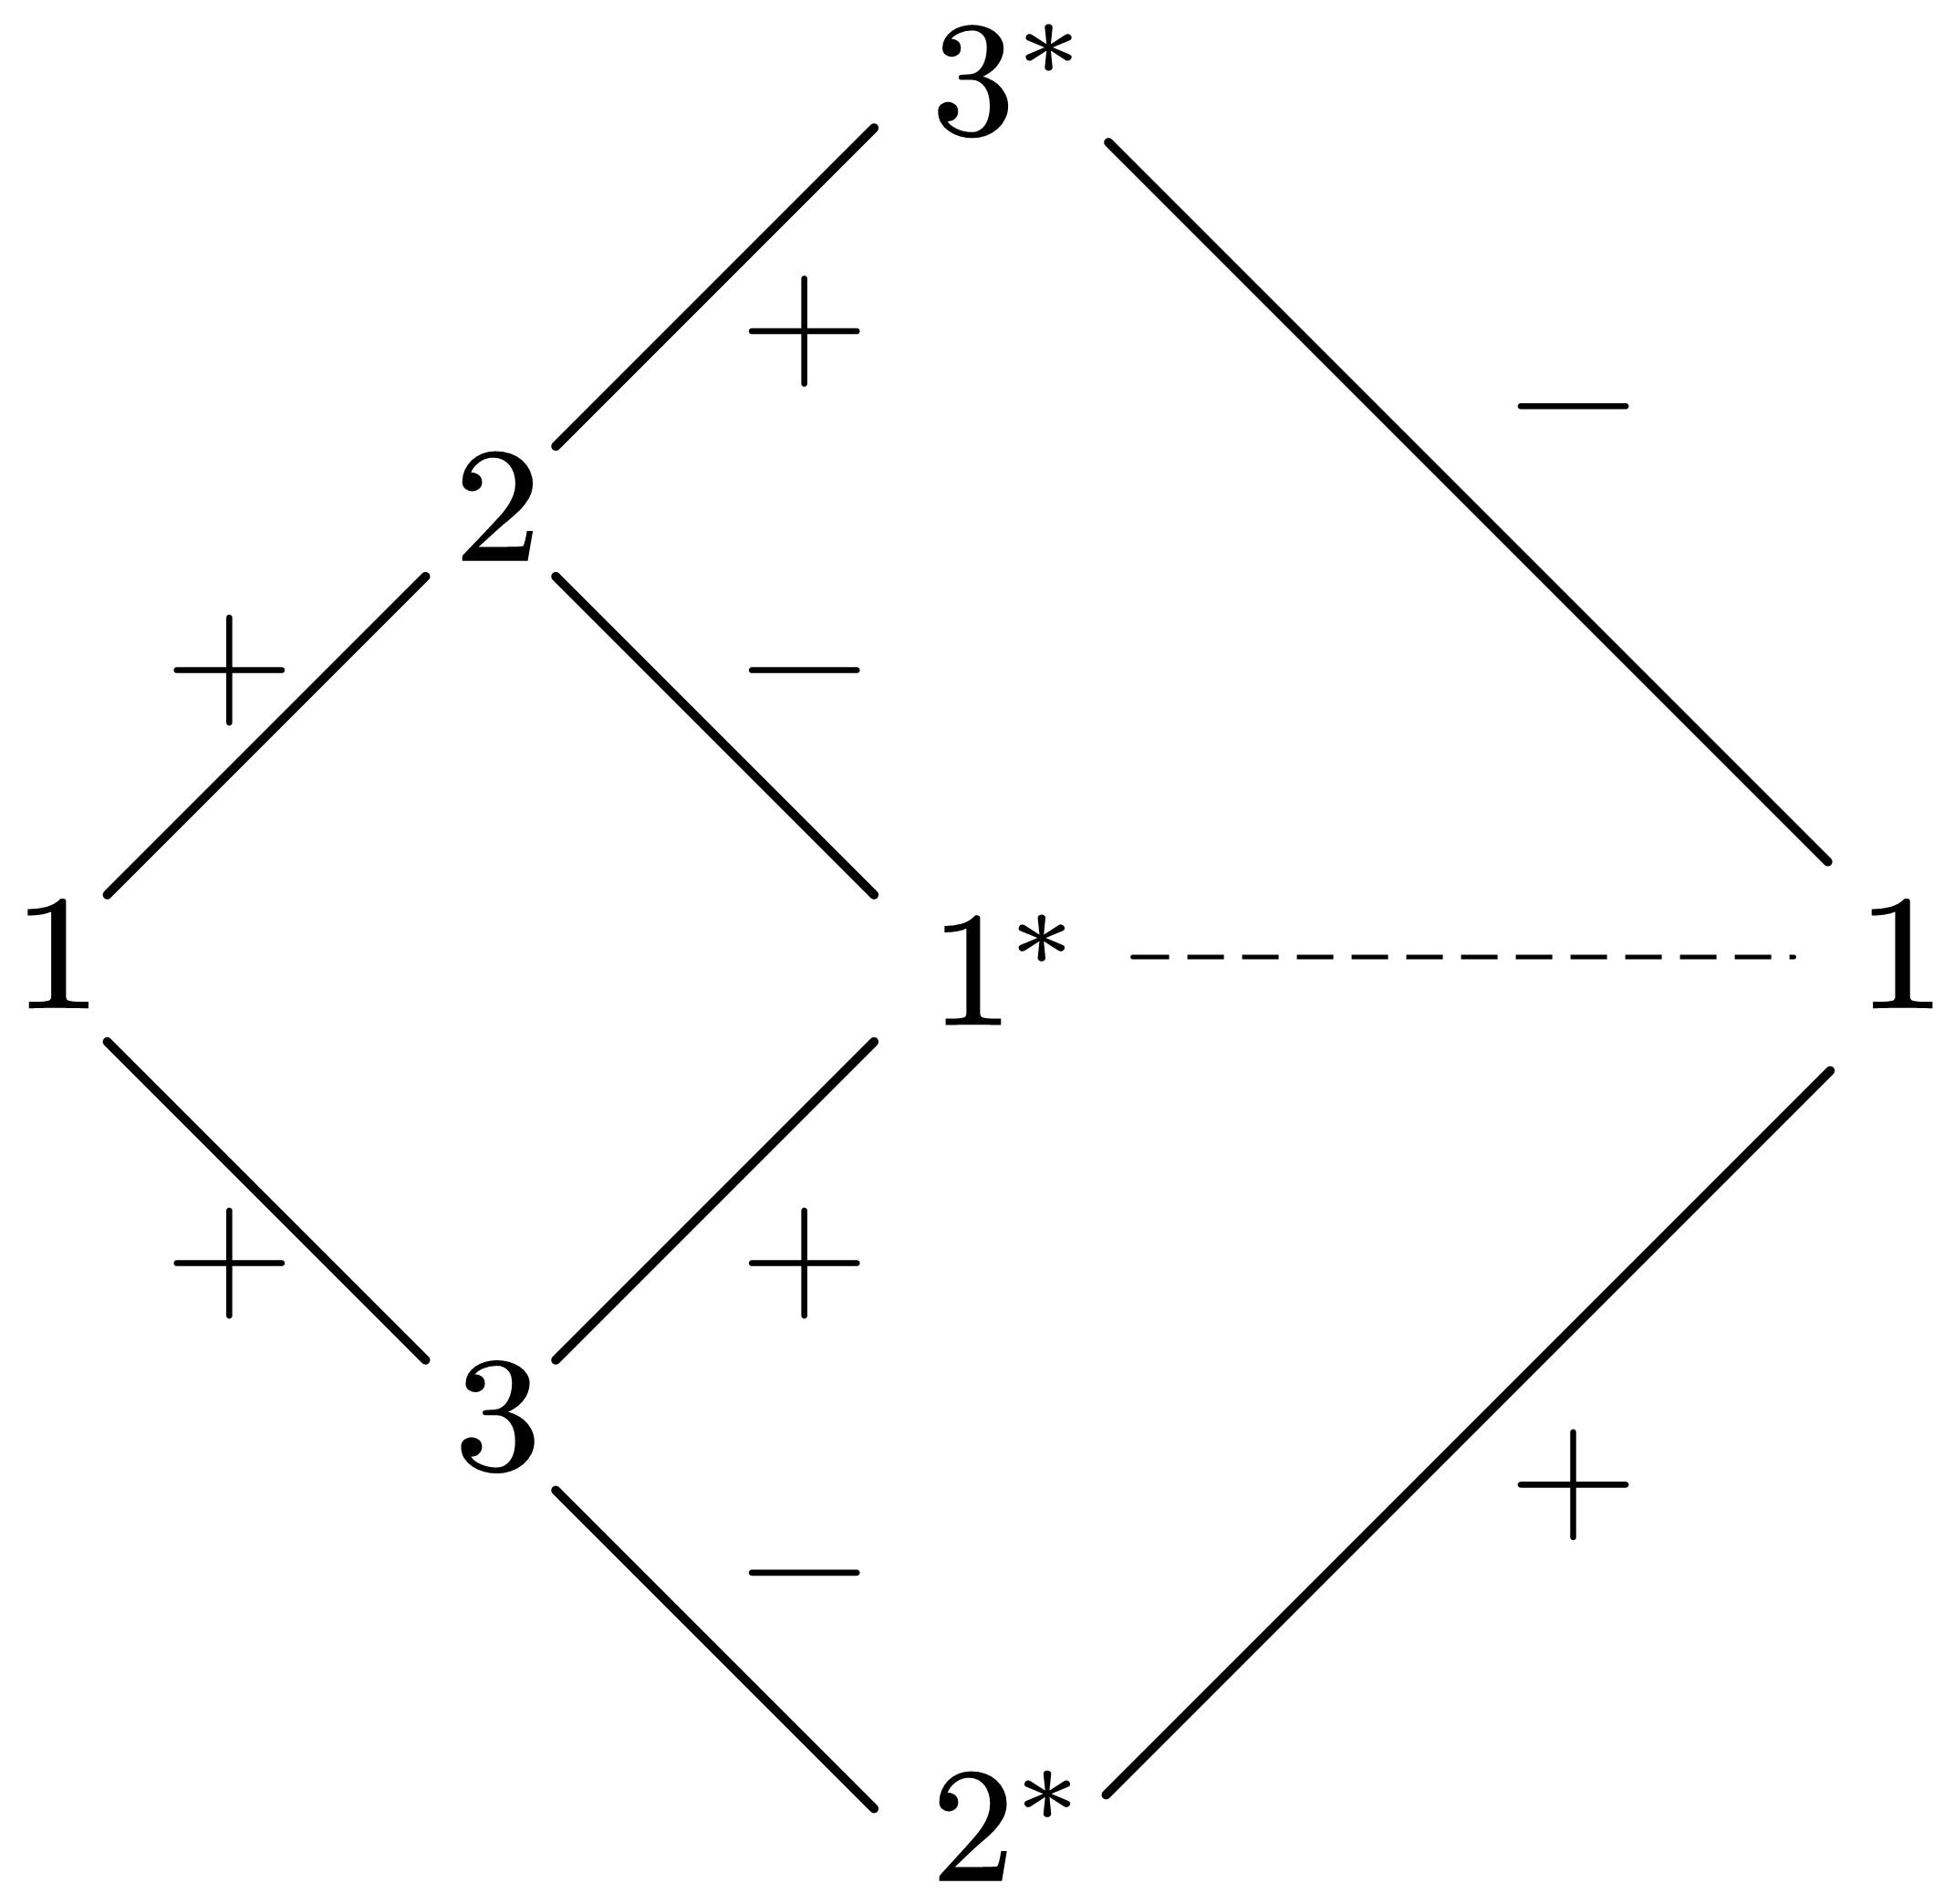
\includegraphics[scale=0.8]{./pictures/6.05/pictorial_representation_1.png}
		\captionof{figure}{Pictorial representation of the second term in $E^{(3)}_0$, where the order is $v_{ij}$, $v_{jk^*}$ and $v_{k^*i}$ from the left to the right. The plus and minus signs indicate whether the matrix elements between the two orbitals is $\pm \frac{\beta}{2}$.}\label{fig:exe5}
	\end{center}
	
	With the high symmetry, it is
	\begin{sequation}
		-2 \times \frac{1}{ (2\beta)^2 } \sum_{i=1}^3 \left[ v_{12} v_{23^*} v_{3^*1} + v_{13} v_{32^*} v_{2^*1} \right] = - \frac{3}{ 2\beta^2 } \left[ \frac{ \beta }{2} \times \frac{ \beta }{2} \times \left( - \frac{ \beta }{2} \right) + \frac{ \beta }{2} \times \left( - \frac{ \beta }{2} \right) \times \frac{ \beta }{2} \right] = \frac{3}{8\beta} .
	\end{sequation}	
	
	\end{solution}

	% 6.6
	\begin{exercise}
	Consider a cyclic polyene with $N = 4\nu+2$, $\nu=1$, $2$, ... carbons. Instead of assuming that all the bonds are identical, suppose they alternate in length. In the context of H{\"u}ckel theory this means that the resonance integrals between adjacent carbons are not all equal to $\beta$ but alternate between $\beta_1$ and $\beta_2$. For example, for benzene we have
	
	\begin{center}
	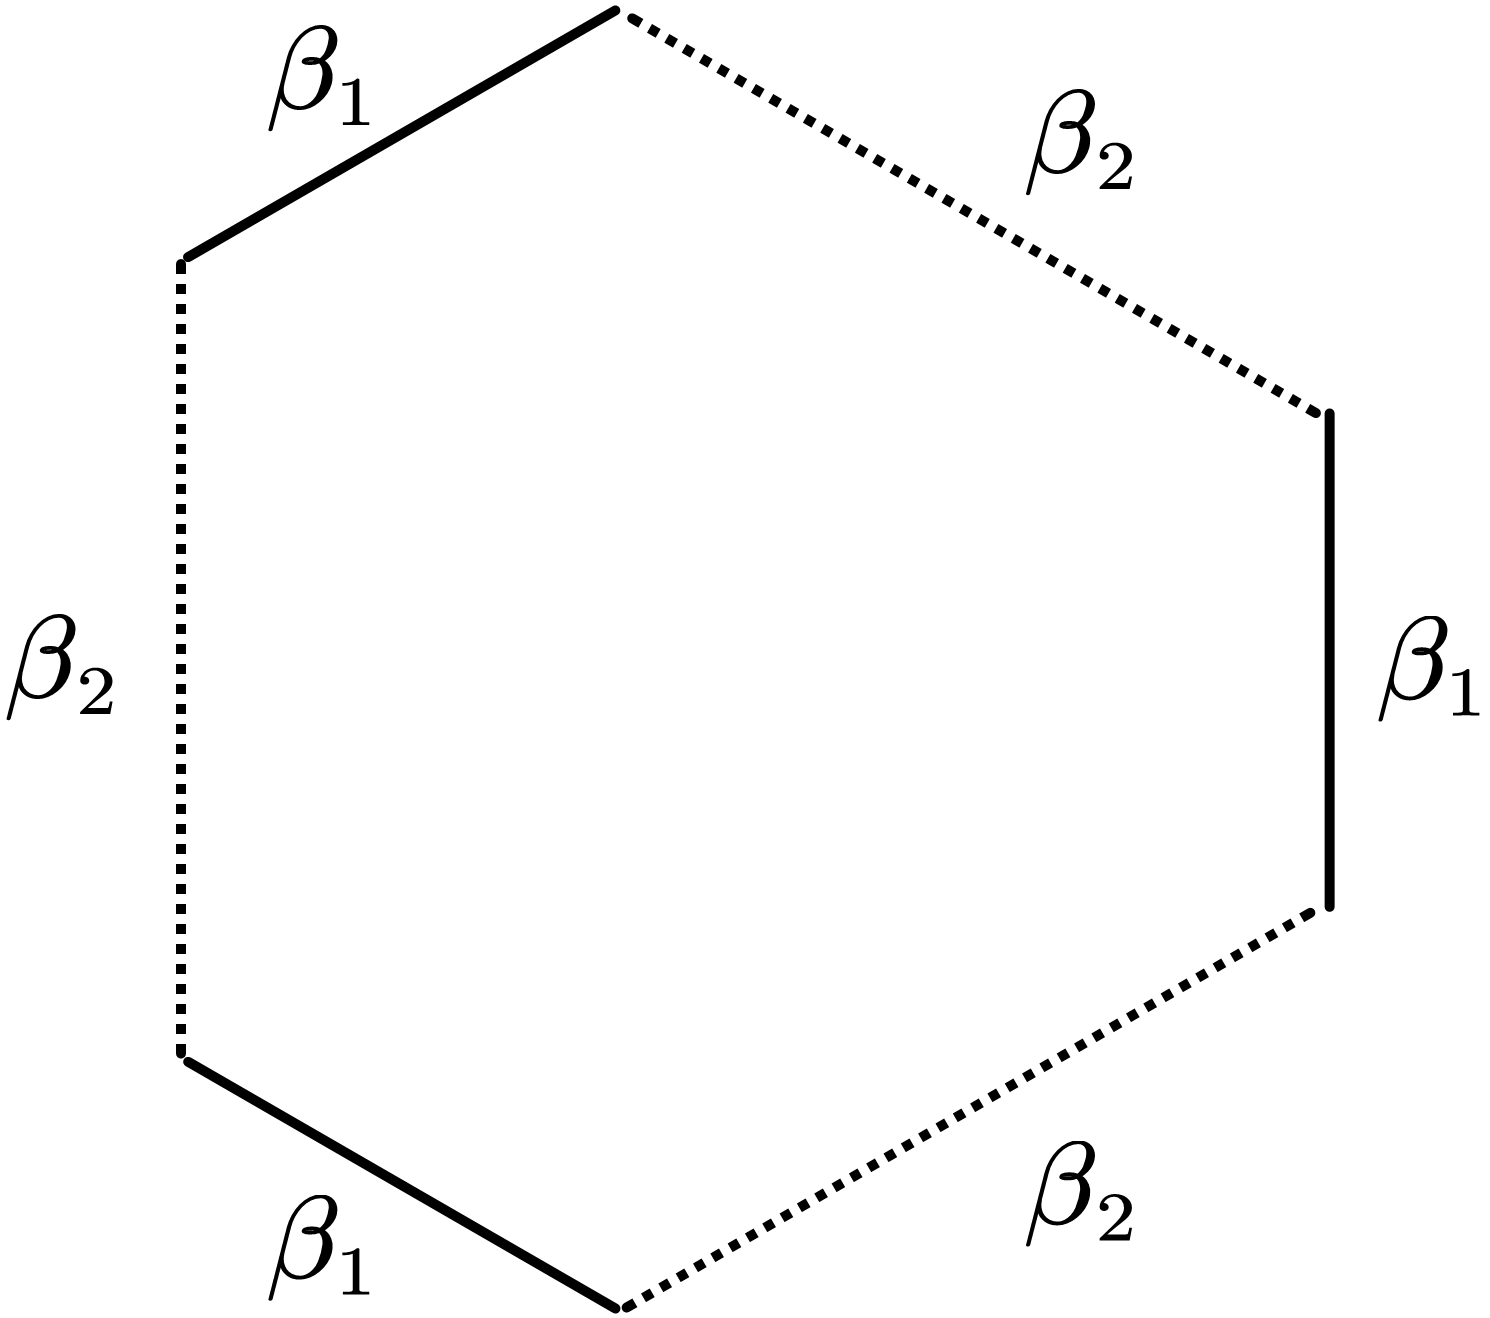
\includegraphics[scale=1.2]{./pictures/6.06/exercise_1.png}
	\end{center}
	
	Now it can be shown that the exact energy for a cyclic polyene of this type is
	\[
		\mathscr{E}_0 = N \alpha - 2 \sum_{j=-\nu}^\nu \left( \beta^2_1 + \beta^2_2 + 2 \beta_1 \beta_2 \cos{\frac{2j\pi}{2\nu+1}} \right)^{1/2}
	\]
	(see for example, L. Salem, {\it Molecular Orbital Theory of Conjugated Systems}, Benjamin, New York, 1966, pp.498-500). Note that when $\beta_1 = \beta_2 = \beta$, since $2\cos^2\theta=(1+\cos2\theta)$ and $\beta$ is negative, we recover
	\[
		\mathscr{E}_0 = N \alpha + 4 \beta \sum_{j=-\nu}^\nu \cos{\frac{j\pi}{2\nu+1}}
	\]
	which is the result quoted in Subsection 5.3.2. Also note that when $\beta_1=\beta$ but $\beta_2=0$, we have
	\[
		\mathscr{E}_0 = N \alpha + N \beta
	\]
	which is just the total energy of the polyene using the localized ethylenic description. The purpose of this exercise is to obtain the perturbation expansion for the resonance energy by expanding the exact energy in powers of $\beta_2/\beta_1$.
	\begin{enumerate}
	
	\item[a.] Show that for benzene ($\nu=1$) the exact ground state energy in the alternating short and long bond model is
	\[
		\mathscr{E}_0 = 6 \alpha + 2(\beta_1 + \beta_2) - 4 ( \beta^2_1 + \beta^2_2 - \beta_1 \beta_2 )^{1/2}
	\]
	Do this first by using the general expression and then by setting up the H{\"u}ckel matrix, diagonalizing it and adding up the occupied orbital energies. Note that when $\beta_1=\beta_2=\beta$ we recover our old result, $6\alpha+8\beta$.
	
	\item[b.] Setting $\beta_1 = \beta$ and $\beta_2/\beta_1=x$ show that the resonance energy of benzene can be written as
	\[
		E_R = 4 \beta ( \frac{1}{2}x - 1 + (1-x+x^2)^{1/2})
	\]
	Note that when $x=0$, $E_R=0$ and when $x=1$, $E_R=2\beta$ which is exact.
	
	\item[c.] Using the relation
	\[
		(1 + y)^{1/2} = 1 + \frac{1}{2} y - \frac{1}{8}y^2 + \frac{1}{16} y^3 - \frac{5}{128}y^4 + \cdots , \quad |y|<1
	\]	
	expand $E_R$ to fourth order in $x$ and thus show that
	\[
		E_R = \beta ( \frac{3}{2}x^2 + \frac{3}{4} x^3 + \frac{3}{32}x^4 + \cdots )
	\]
	Identifying the coefficient of $x^n$ with the $n$th-order perturbation result (i.e., $E^{(n)}_0$), we have
	\begin{align*}
		E^{(2)}_0 &= \frac{3}{2} \beta, \\
		E^{(3)}_0 &= \frac{3}{4} \beta, \\
		E^{(4)}_0 &= \frac{3}{32} \beta.
	\end{align*}
	Note that $E^{(2)}_0$ and $E^{(3)}_0$ agree with our previously calculated values. This derivation provides some insight into the poor convergence of the perturbation expansion of the resonance energy of benzene. Basically, the perturbation expansion converges rapidly when $x$ is small. However, for our problem $x$ is equal to unity.
	
	The resonance energy calculated up to $M$th-order as a function of $M$ is shown below. Note the oscillatory convergence towards the exact value of $2\beta$. The method used above to obtain $E^{(n)}_0$ for $n=2,3,4$ becomes extremely laborious for larger $n$. The results below were calculated by first showing that $E^{(n)}_0 = 4\beta C^{-1/2}_n(1/2)$, where $C^{-1/2}_n(x)$ is a Gegenbauer polynomial of degree $n$ and order $-\frac{1}{2}$, and then using the recursive properties of these polynomials, to show that
	\[
		(n+1)E^{(n+1)}_0 = (n-1) E^{(n)}_0 - (n-2) E^{(n-1)}_0.
	\]
	
	\begin{center}
	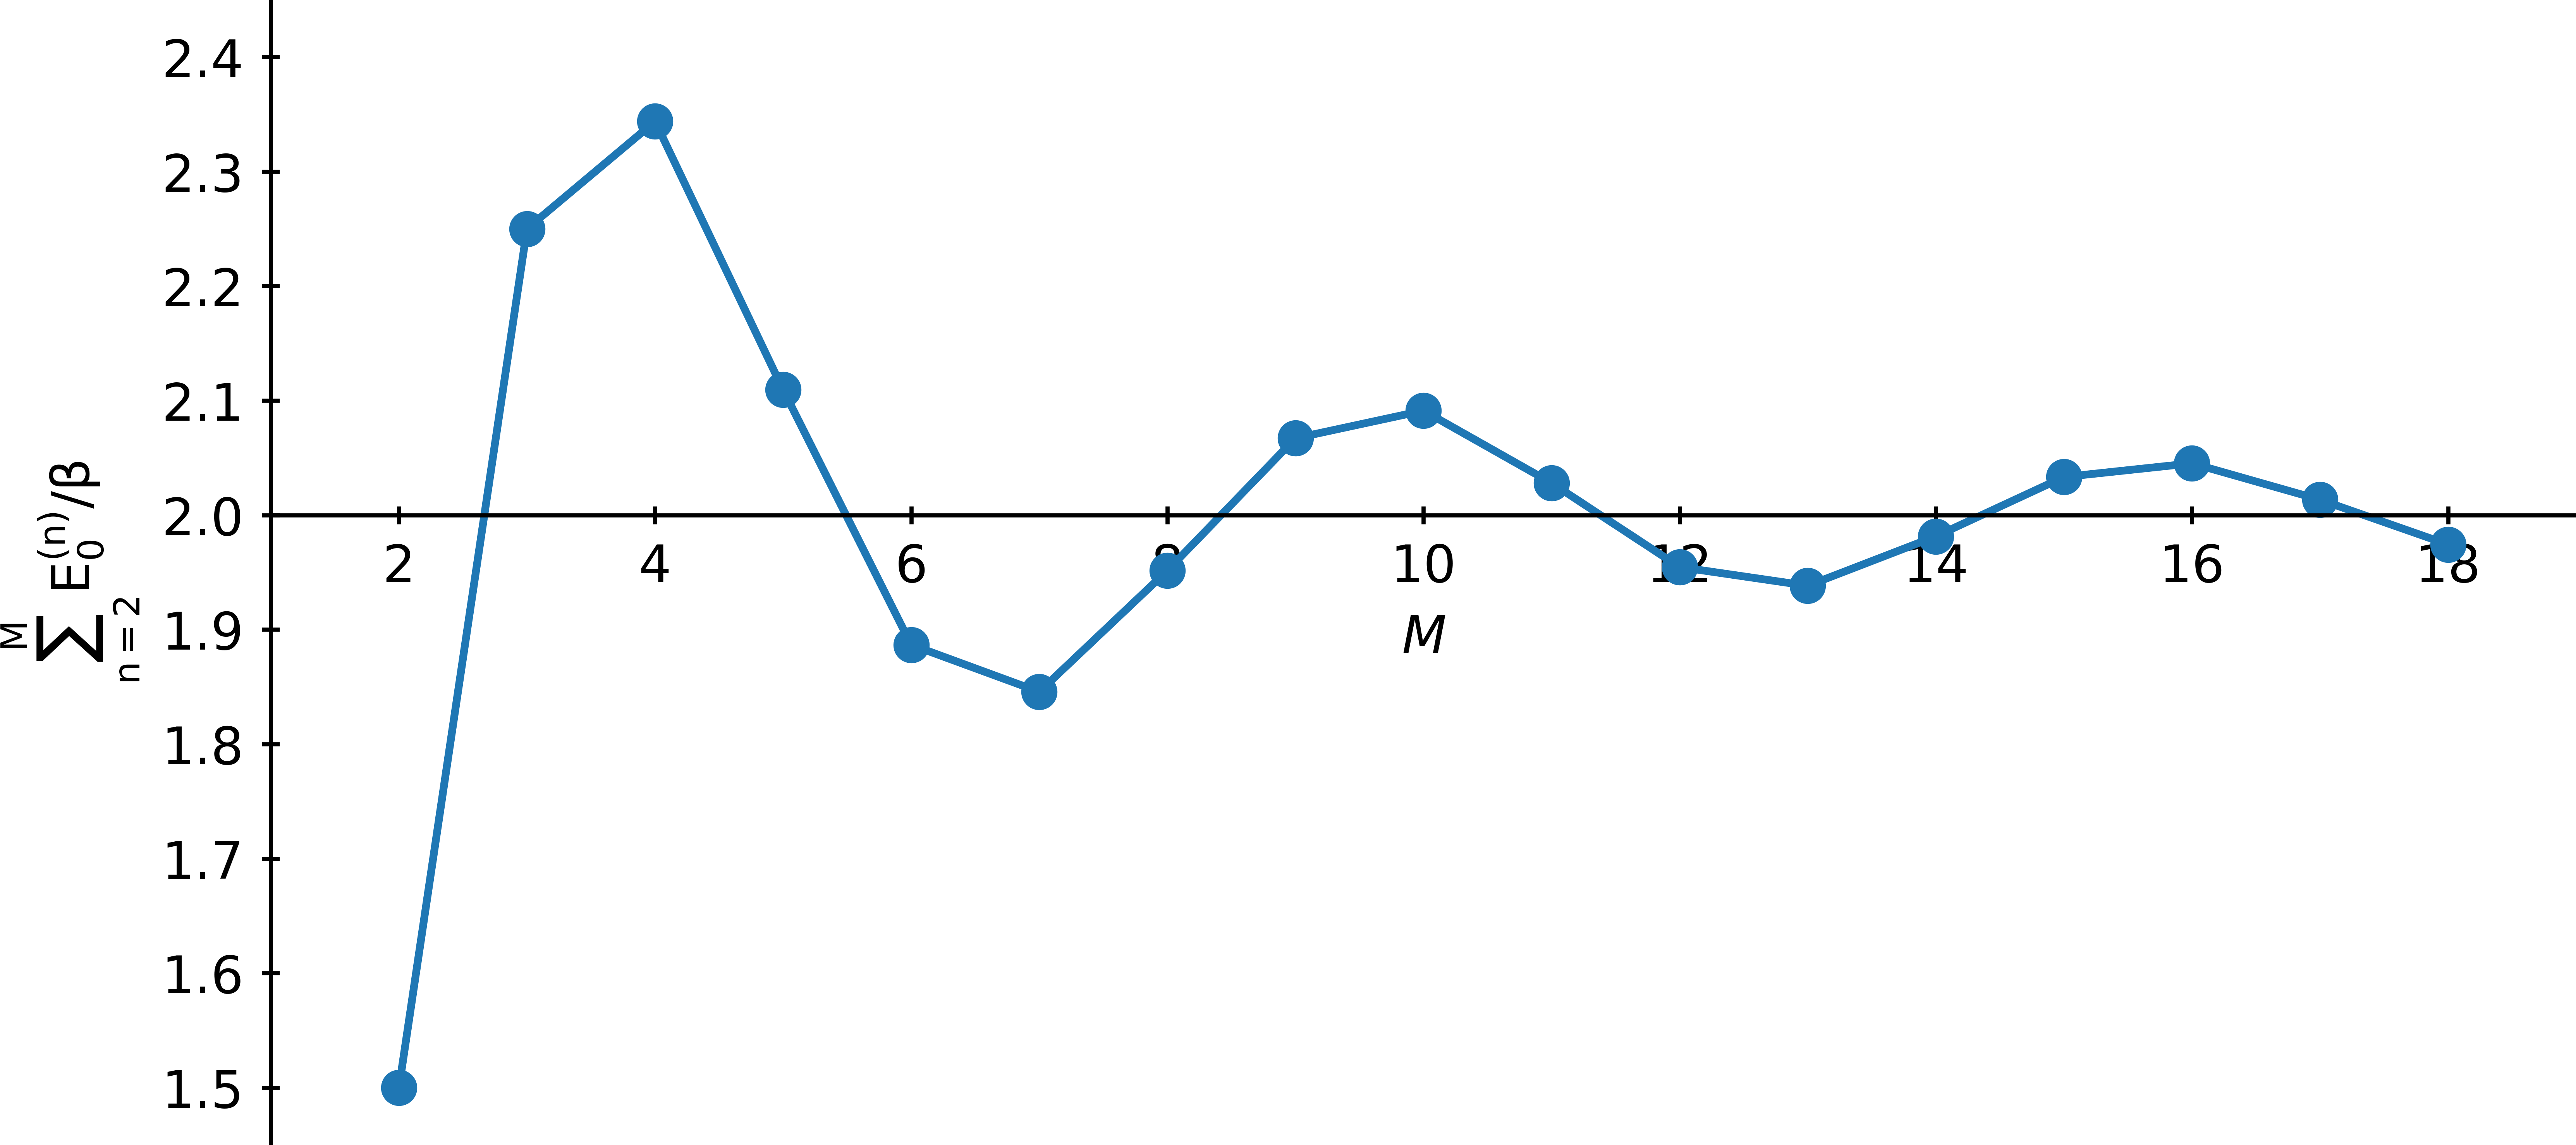
\includegraphics[scale=0.84]{./pictures/6.06/gegenbauer.png}
	\end{center}
	
	\end{enumerate}
	
	\end{exercise}
	
	\begin{solution}

	\begin{itemize}
	
	\item[a.] Using the general expression and note that $\beta_1 \le 0$ and $\beta_2 \le 0$, we get that
	\begin{align*}
		\mathscr{E}_0({\rm benzene}) &= 6 \times \alpha - 2 \sum_{ j=-1 }^1 \left( \beta^2_1 + \beta^2_2 + 2 \beta_1 \beta_2 \cos{\frac{2j\pi}{ 2 \times 1 + 1 }} \right)^{1/2} \\
		&= 6\alpha - 2 \left( \beta^2_1 + \beta^2_2 + 2 \beta_1 \beta_2 \cos{\frac{-2\pi}{ 3 }} \right)^{1/2} \\
		&\hspace{2em} - 2 \left( \beta^2_1 + \beta^2_2 + 2 \beta_1 \beta_2 \cos{\frac{0\pi}{ 3 }} \right)^{1/2} - 2 \left( \beta^2_1 + \beta^2_2 + 2 \beta_1 \beta_2 \cos{\frac{2\pi}{ 3 }} \right)^{1/2} \\
		&= 6\alpha - 2\left( \beta^2_1 + \beta^2_2 - \beta_1 \beta_2 \right)^{1/2} + 2\left( \beta_1 + \beta_2 \right) - 2\left( \beta^2_1 + \beta^2_2 - \beta_1 \beta_2 \right)^{1/2}.
	\end{align*}
	In a nut shell,
	\begin{sequation}
		\mathscr{E}_0({\rm benzene}) = 6\alpha + 2\left( \beta_1 + \beta_2 \right) - 4\left( \beta^2_1 + \beta^2_2 - \beta_1 \beta_2 \right)^{1/2} .
	\end{sequation}
	
	At this time, we should remember that the H{\"u}ckel matrix is 
	\[
		\HH = \begin{pmatrix}
			\alpha & \beta_2 & 0 & 0 & 0 & \beta_1 \\
			\beta_2& \alpha  & \beta_1 & 0 & 0 & 0 \\
			0 & \beta_1& \alpha  & \beta_2 & 0 & 0 \\
			0 & 0 & \beta_2& \alpha  & \beta_1 & 0 \\
			0 & 0 & 0 & \beta_1& \alpha  & \beta_2 \\
			\beta_1 & 0 & 0 & 0 & \beta_2 & \alpha
		\end{pmatrix}.
	\]
	Its eigen function is
	\[
		\det{\HH-\varepsilon\I} = (\beta^2_1 - \beta_1 \beta_2 + \beta^2_2 - (\alpha - \varepsilon)^2)^2 (\alpha - \beta_1 - \beta_2 - \varepsilon) (\alpha + \beta_1 + \beta_2 - \varepsilon) = 0,
	\]
	and there are six roots:
	\begin{align*}
		\varepsilon_1 &= \alpha + \beta_1 + \beta_2 , \\
		\varepsilon_2 = \varepsilon_3 &= \alpha - \sqrt{ \beta^2_1 - \beta_1 \beta_2 + \beta^2_2 }, \\
		\varepsilon_4 = \varepsilon_5 &= \alpha + \sqrt{ \beta^2_1 - \beta_1 \beta_2 + \beta^2_2 }, \\
		\varepsilon_6 &= \alpha - \beta_1 - \beta_2 .
	\end{align*}
	Thus,
	\begin{sequation}
		\mathscr{E}^\prime_0({\rm benzene}) = 2\varepsilon_1 + 2\varepsilon_2 + 2\varepsilon_3 = 6\alpha + 2\left( \beta_1 + \beta_2 \right) - 4\left( \beta^2_1 + \beta^2_2 - \beta_1 \beta_2 \right)^{1/2} .
	\end{sequation}
	It equals the results obtained by using the general expression.
	
	\item[b.] The verification is direct. With $\beta_1 = \beta$, $\beta_2 = x\beta_1 = x\beta$, we get that
	\begin{align*}
		E_R &= \mathscr{E}_0({\rm benzene}) - E_0 = 6\alpha + 2\left( \beta + x \beta \right) - 4\left( \beta^2 + ( x \beta )^2 - x \beta^2 \right)^{1/2} - ( 6\alpha + 6\beta ) \\
		&= -4\beta + 2x \beta + 4\beta \left( 1 + x^2 - x \right)^{1/2} = 4\beta \left( \frac{x}{2} - 1 + \left( 1 + x^2 - x \right)^{1/2} \right)
	\end{align*}
	
	\item[c.] When $0 \le x \le 1$, $-\frac{1}{4} \le x^2-x \le 0$, thus we obtain that
	\begin{align*}
		E_R &= 4\beta \left( \frac{x}{2} - 1 + \left( 1 + x^2 - x \right)^{1/2} \right) = 4\beta \left[ \frac{x}{2} - 1 + \left( 1 + \left( x^2 - x \right) \right)^{1/2} \right] \\
		&= 4\beta \left[ \frac{x}{2} - 1 + 1 + \frac{1}{2} \left( x^2 - x \right) - \frac{1}{8} \left( x^2 - x \right)^2 + \frac{1}{16} \left( x^2 - x \right)^3 - \frac{5}{128} \left( x^2 - x \right)^4 + \cdots \right] \\
		&= 4\beta \left[ \frac{x}{2} + \frac{1}{2} \left( - x + x^2 \right) - \frac{1}{8} \left( x^2 - 2 x^3 + x^4 \right)  \right. \\
		&\hspace{4em} \left. + \frac{1}{16} \left( - x^3 + 3 x^4 - 3 x^5 + x^6 \right) - \frac{5}{128} \left( x^4 - 4x^5 + 6x^6 - 4x^7 + x^8 \right) + \cdots \right] \\
		&= 4\beta \left[ \left( \frac{1}{2} - \frac{1}{2} \right) x + \left( \frac{1}{2} - \frac{1}{8} \right) x^2 + \left( \frac{1}{4} - \frac{1}{16} \right) x^3 + \left( - \frac{1}{8} + \frac{3}{16} - \frac{5}{128} \right) x^4 + \cdots \right] \\
		&= \beta \left( \frac{3}{2} x^2 + \frac{3}{4} x^3 + \frac{3}{32} x^4 + \cdots \right) .
	\end{align*}
	
	In fact, the Gegenbauer polynomials $C^\lambda_n(x)$ can be generated by $(1-2xt+t^2)^{-\lambda}$, viz.,
	\[
		(1-2xt+t^2)^{-\lambda} = \sum_{ n=0 }^\infty C^\lambda_n (x) t^n, \, \forall t \in (-1,1), x \in (-1,1).
	\]
	Let $\lambda=-\frac{1}{2}$ and $x=\frac{1}{2}$, we obtain that
	\[
		( 1 - t + t^2 )^{\frac{1}{2}} = \sum_{ n=0 }^\infty C^{-\frac{1}{2}}_n \left( \frac{1}{2} \right) t^n.
	\]
	Thus, with 
	\[
		C^\lambda_0(x) = 1 , \quad C^\lambda_1(x) = 2 \lambda x ,
	\]	
	we find that	
	\[
		\sum_{ n=0 }^\infty C^{-\frac{1}{2}}_n \left( \frac{1}{2} \right) t^n = C^{-\frac{1}{2}}_0 \left( \frac{1}{2} \right) + C^{-\frac{1}{2}}_0 \left( \frac{1}{2} \right) t + \sum_{ n=2 }^\infty C^{-\frac{1}{2}}_n \left( \frac{1}{2} \right) t^n = 1 - \frac{t}{2} + \sum_{ n=2 }^\infty C^{-\frac{1}{2}}_n \left( \frac{1}{2} \right) t^n.
	\]
	
	Hence, we get
	\begin{sequation}
		E_R = 4\beta \left( \frac{x}{2} - 1 + \left( 1 - x + x^2 \right)^{1/2} \right) = 4\beta \sum_{ n=2 }^\infty C^{-\frac{1}{2}}_n \left( \frac{1}{2} \right) x^n.
	\end{sequation}
	It equals
	\begin{sequation}
		E^{(n)}_0 = 4\beta C^{-\frac{1}{2}}_n \left( \frac{1}{2} \right), \, n = 2, 3, 4, \cdots.
	\end{sequation}
	
	Due to the recurrence relation of Gegenbauer polynomials,
	\[
		(n+1)C^\lambda_{n+1}(x) = 2(n+\lambda) x C^\lambda_n(x) - ( n + 2\lambda - 1 ) C^\lambda_{n-1}(x), \, \forall n \ge 1, 
	\]
	we know that for $n=2,3,\cdots$,
	\begin{align*}
		(n+1)E^{(n+1)}_0 &= (n+1) \times 4\beta C^{-\frac{1}{2}}_{n+1} \left( \frac{1}{2} \right) = 4\beta (n+1) C^{-\frac{1}{2}}_{n+1} \left( \frac{1}{2} \right) \\
		&= 4\beta \left[ 2\left( n - \frac{1}{2} \right) \frac{1}{2} C^{ -\frac{1}{2} }_n \left( \frac{1}{2} \right) - \left( n + 2 \times \left( -\frac{1}{2} \right) - 1 \right) C^{ -\frac{1}{2} }_{n-1}\left( \frac{1}{2} \right) \right] \\
		&= 4\beta \left[ \left( n - \frac{1}{2} \right) C^{ - \frac{1}{2} }_n\left( \frac{1}{2} \right) - ( n - 2 ) C^{ - \frac{1}{2}}_{n-1}\left( \frac{1}{2} \right) \right] \\
		&= \left( n - \frac{1}{2} \right) 4\beta C^{ -\frac{1}{2} }_n\left( \frac{1}{2} \right) - ( n - 2 ) 4\beta C^{ -\frac{1}{2} }_{n-1}\left( \frac{1}{2} \right) \\
		&= \left( n - \frac{1}{2} \right) E^{(n)}_0 - ( n - 2 ) E^{(n-1)}_0.
	\end{align*}
	
	\end{itemize}
	
	Remark: You can read some introduction about Gegenbauer polynomials from WIKIPEDIA, whose url is \url{https://en.wikipedia.org/wiki/Gegenbauer_polynomials}.	
		
	\end{solution}
	
	\sectionstar{Diagrammatic Representation of Orbital Perturbation Theory}
	
	% 6.7
	\begin{exercise}
	Find the fourth-order energy for a closed-shell cyclic polyene.
	\begin{enumerate}
	
	\item[a.] Show that
	
	\begin{center}
	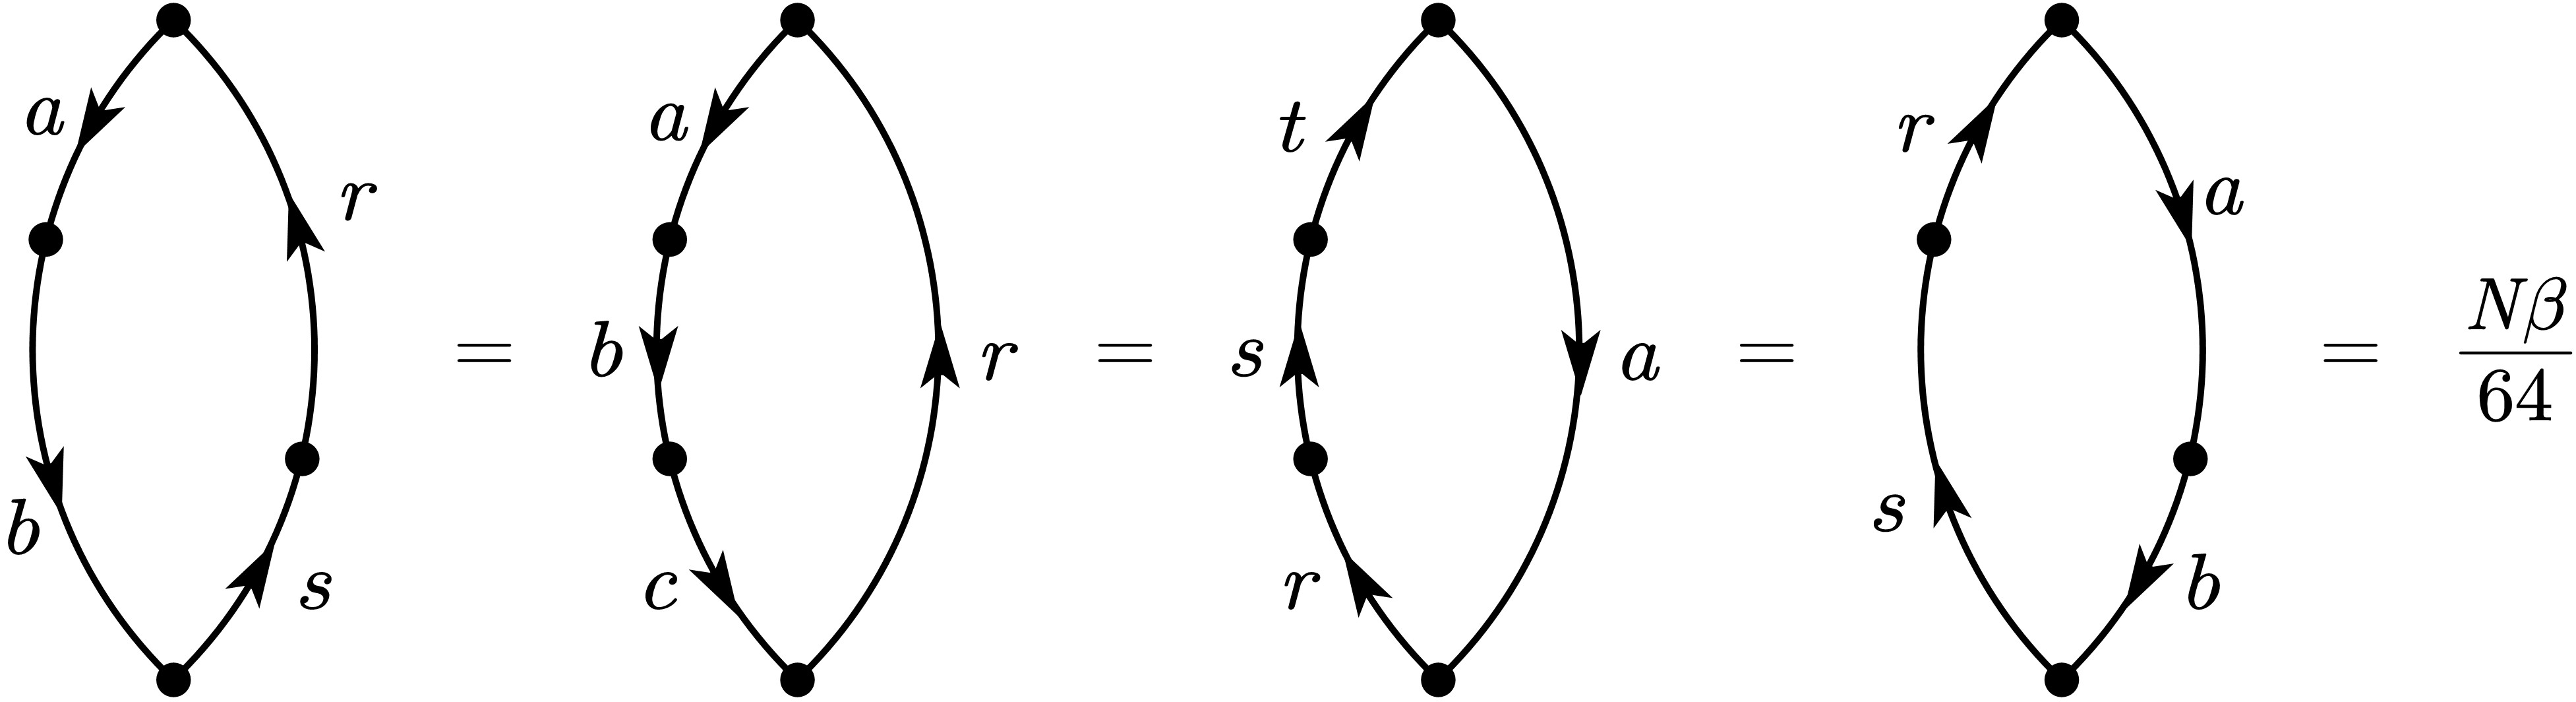
\includegraphics[scale=0.84]{./pictures/6.07/exercise_1.png}
	\end{center}
	
	and
	
	\begin{center}
	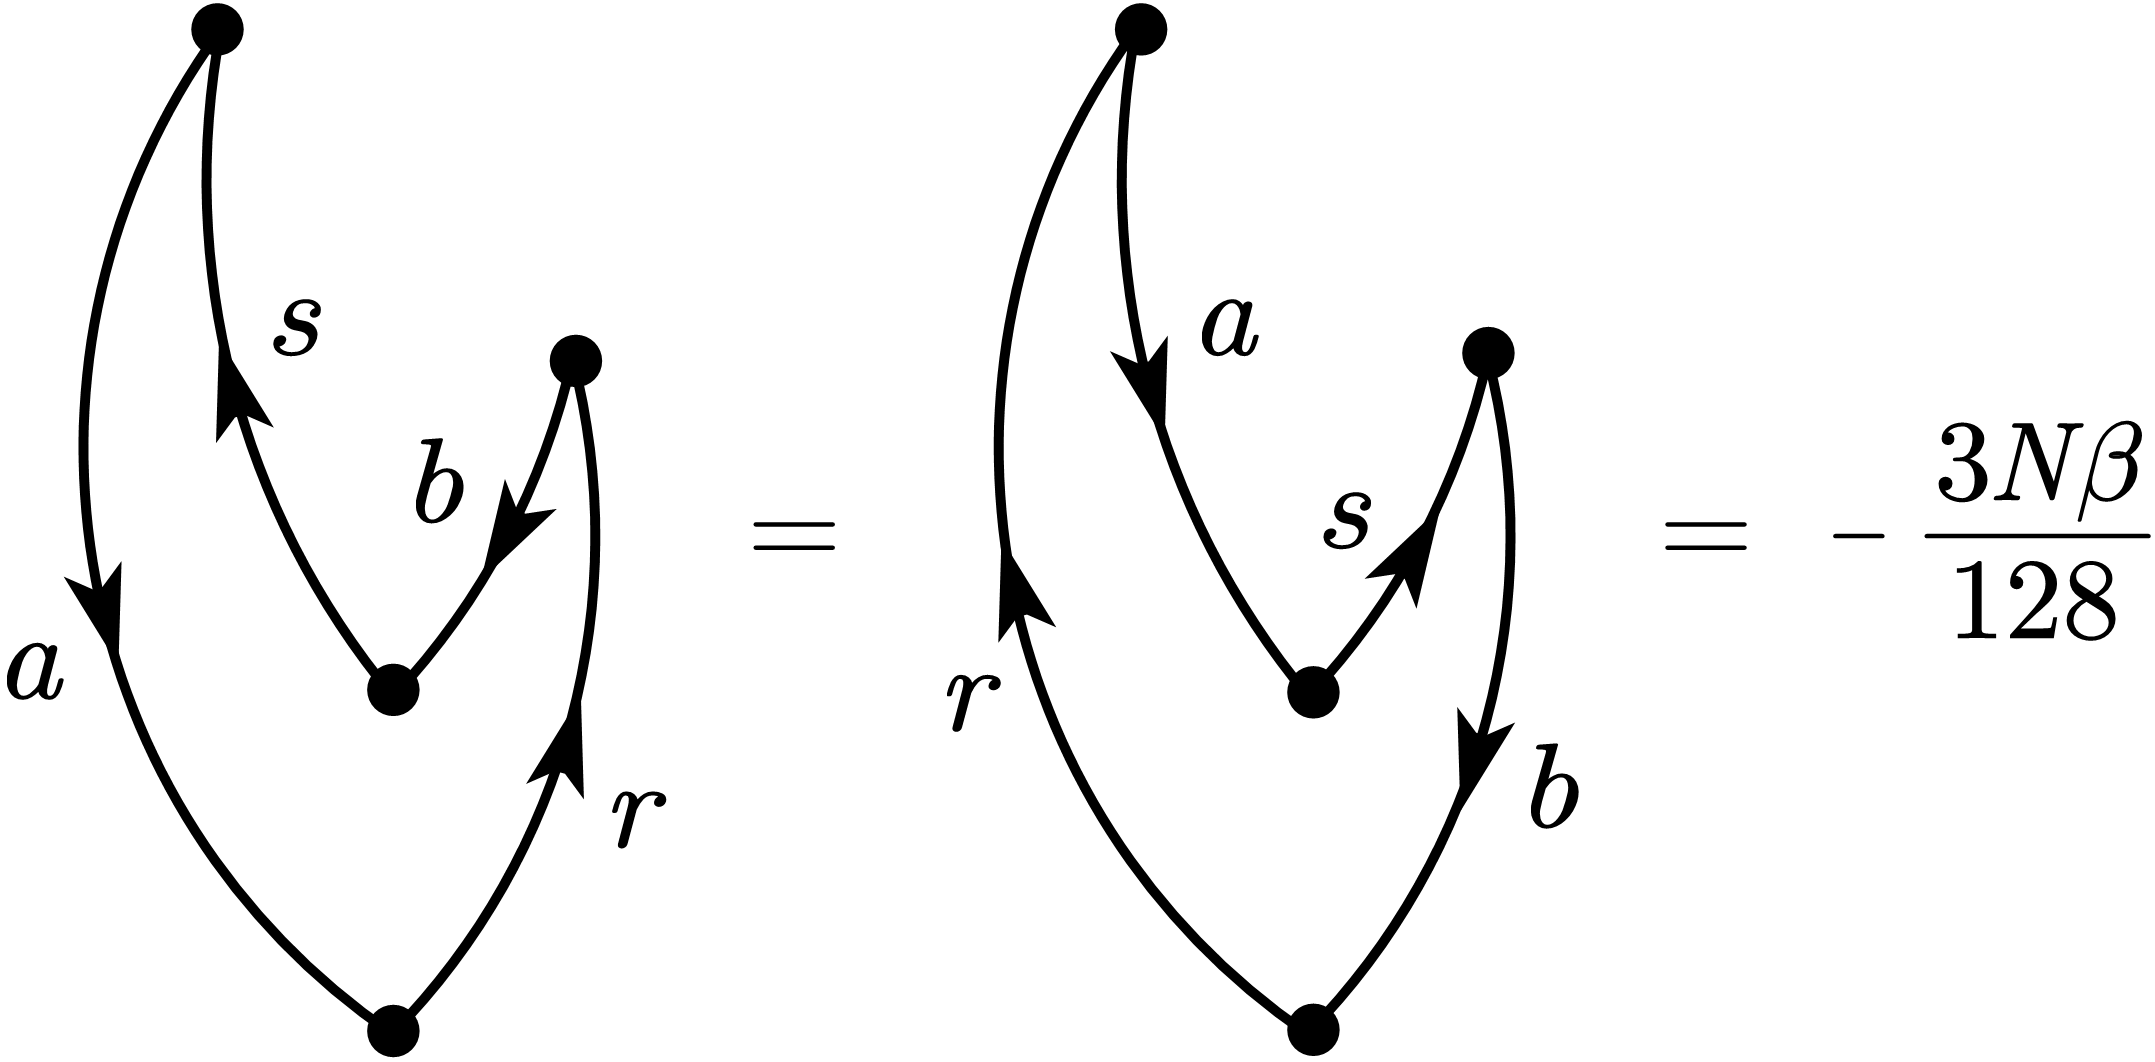
\includegraphics[scale=0.84]{./pictures/6.07/exercise_2.png}
	\end{center}
	
	so that
	\[
		E^{(4)}_0 = \frac{N\beta}{64}
	\]
	Thus the resonance energy calculated for a cyclic polyene with $N>6$ up to fourth order is (1/4 + 1/64)$N\beta = 0.2656N\beta$, which compares very favorably with the asymptotically exact value of 0.2732$\beta$ (i.e., 97\%).
	
	\item[b.] For benzene, show that the diagrammatic result for the fourth-order energy agrees with the independently calculated result found in Exercise 6.6.
	
	\end{enumerate}		
	
	\end{exercise}
	
	\begin{solution}
	
	\begin{itemize}	
	
	\item[a.] Firstly, we list all diagrams of the fourth-order energy. 	
	\begin{center}
	\begin{tabular}{ccc}
	
		\begin{minipage}{0.22\linewidth}
		\centering
		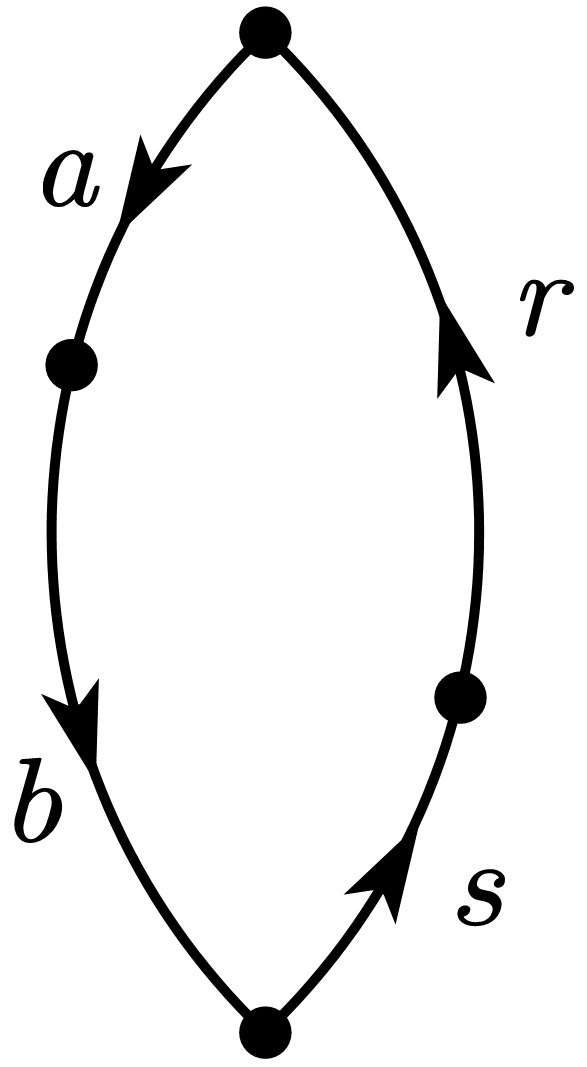
\includegraphics[scale=1.0,trim=0 -4 0 -4]{./pictures/6.07/diagram_1.png}
		\end{minipage} &
		
		\begin{minipage}{0.22\linewidth}
		\centering
		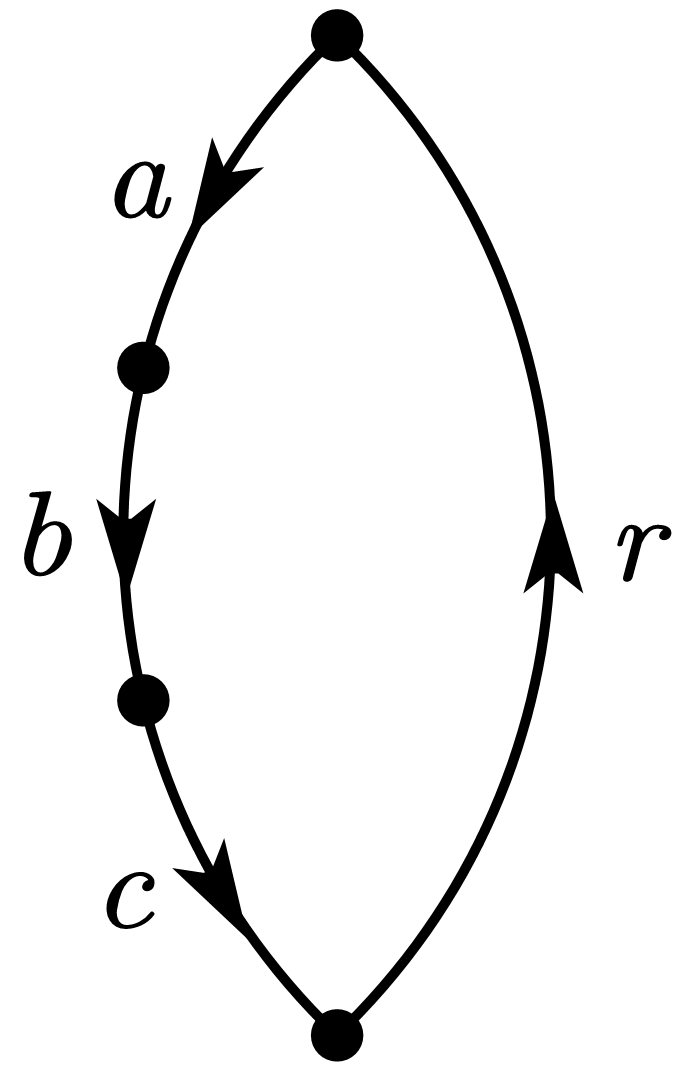
\includegraphics[scale=1.0,trim=0 -4 0 -4]{./pictures/6.07/diagram_2.png}
		\end{minipage} &
		
		\begin{minipage}{0.22\linewidth}
		\centering
		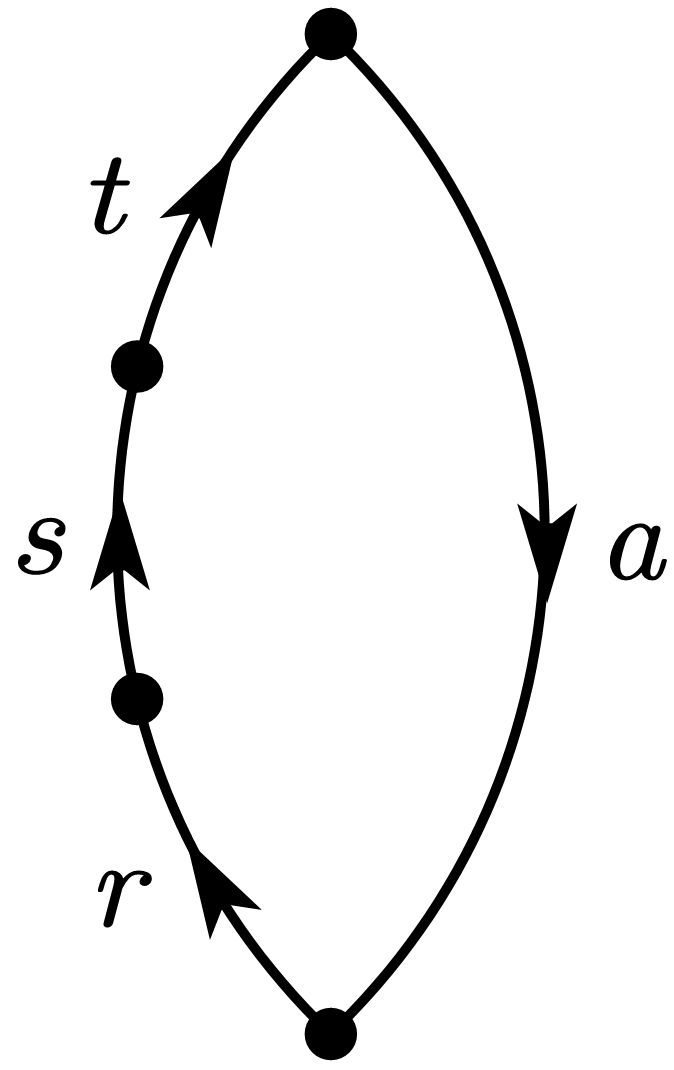
\includegraphics[scale=1.0,trim=0 -4 0 -4]{./pictures/6.07/diagram_3.png}
		\end{minipage} \\
		
		\begin{minipage}{0.22\linewidth}
		\centering
		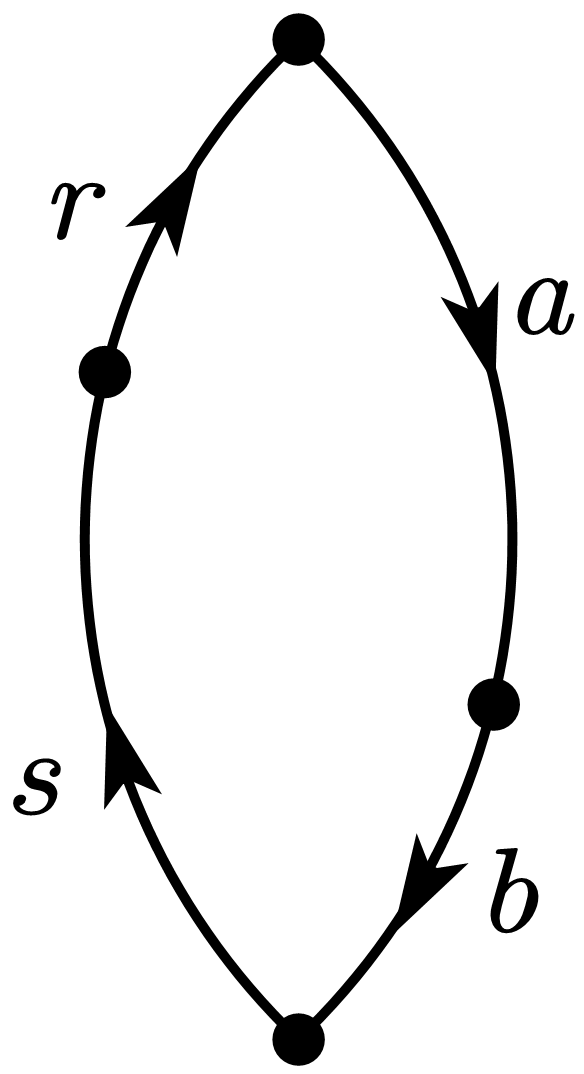
\includegraphics[scale=1.0,trim=0 -4 0 -4]{./pictures/6.07/diagram_4.png}
		\end{minipage} &
			
		\begin{minipage}{0.22\linewidth}
		\centering
		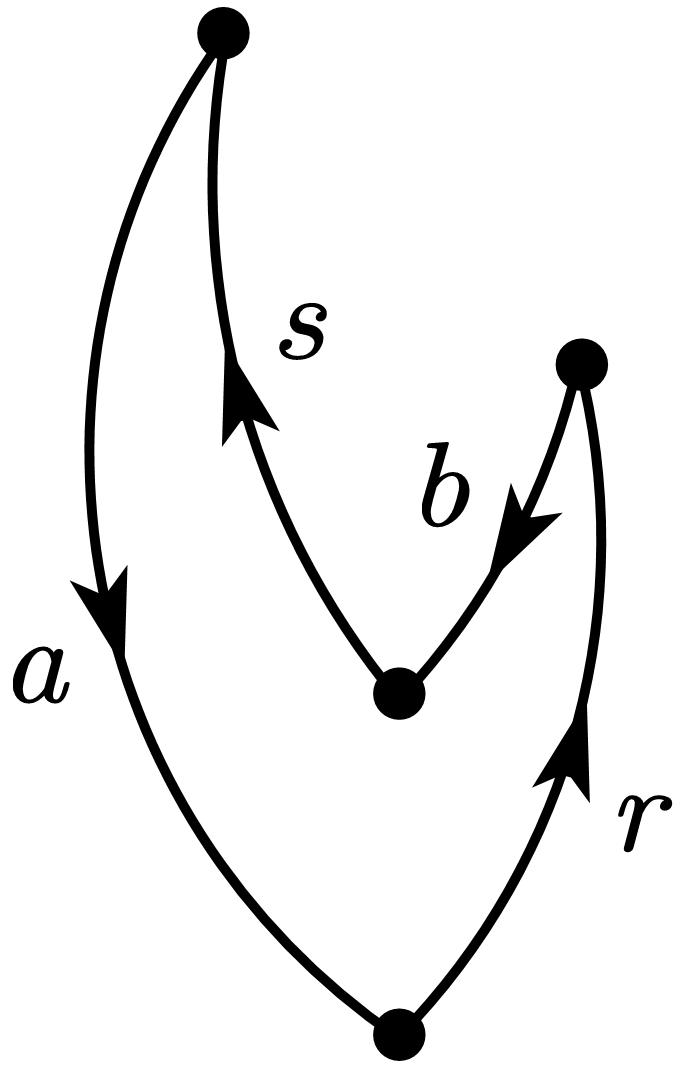
\includegraphics[scale=1.0,trim=0 -4 0 -4]{./pictures/6.07/diagram_5.png}
		\end{minipage} &
		
		\begin{minipage}{0.22\linewidth}
		\centering
		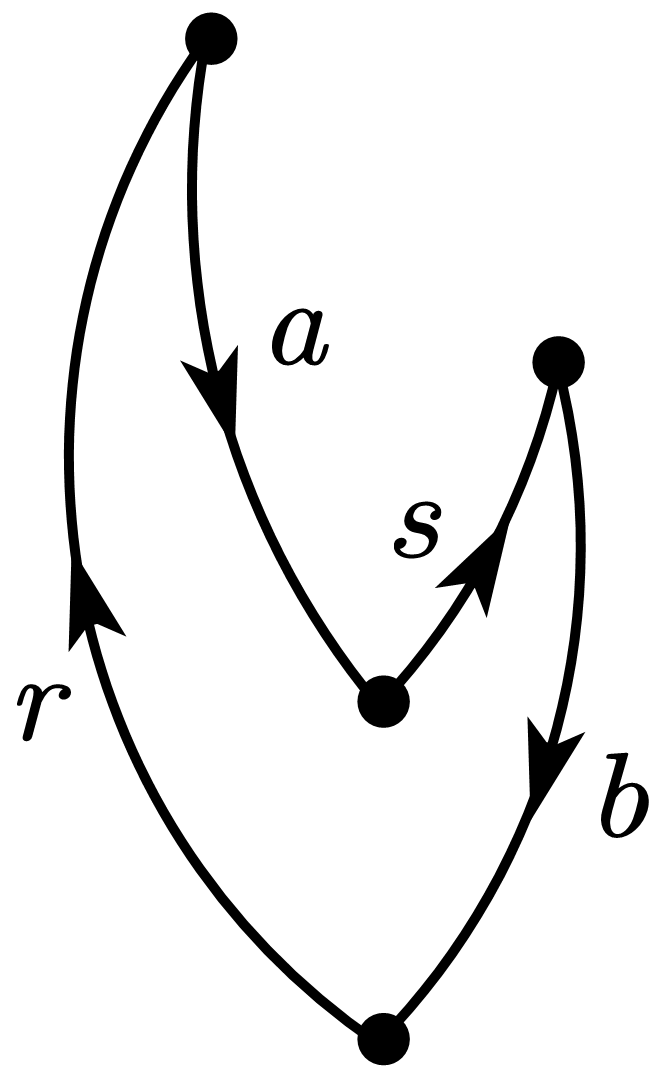
\includegraphics[scale=1.0,trim=0 -4 0 -4]{./pictures/6.07/diagram_6.png}
		\end{minipage}
		
	\end{tabular}
	\captionof{figure}{All fourth-order diagrams.}\label{fig:exe7_1}
	\end{center}
	
	Note that when $N>6$, $(i+3)^*$ cannot interact with $i$, and when $N=6$, $1^*$ cannot interact with $1$, either. Thus, there is no essential difference in the shape and properties between the case of $N > 6$ and $N=6$. It is enough to draw the pictorial representation of benzene ($N=6$) in order to get the same result of $N>6$. The pictorial representation of benzene can be seen in \Figref{fig:exe7_2}.
	
	\begin{center}
	\begin{tabular}{ccc}
	
		\begin{minipage}{0.3\linewidth}
		\centering
		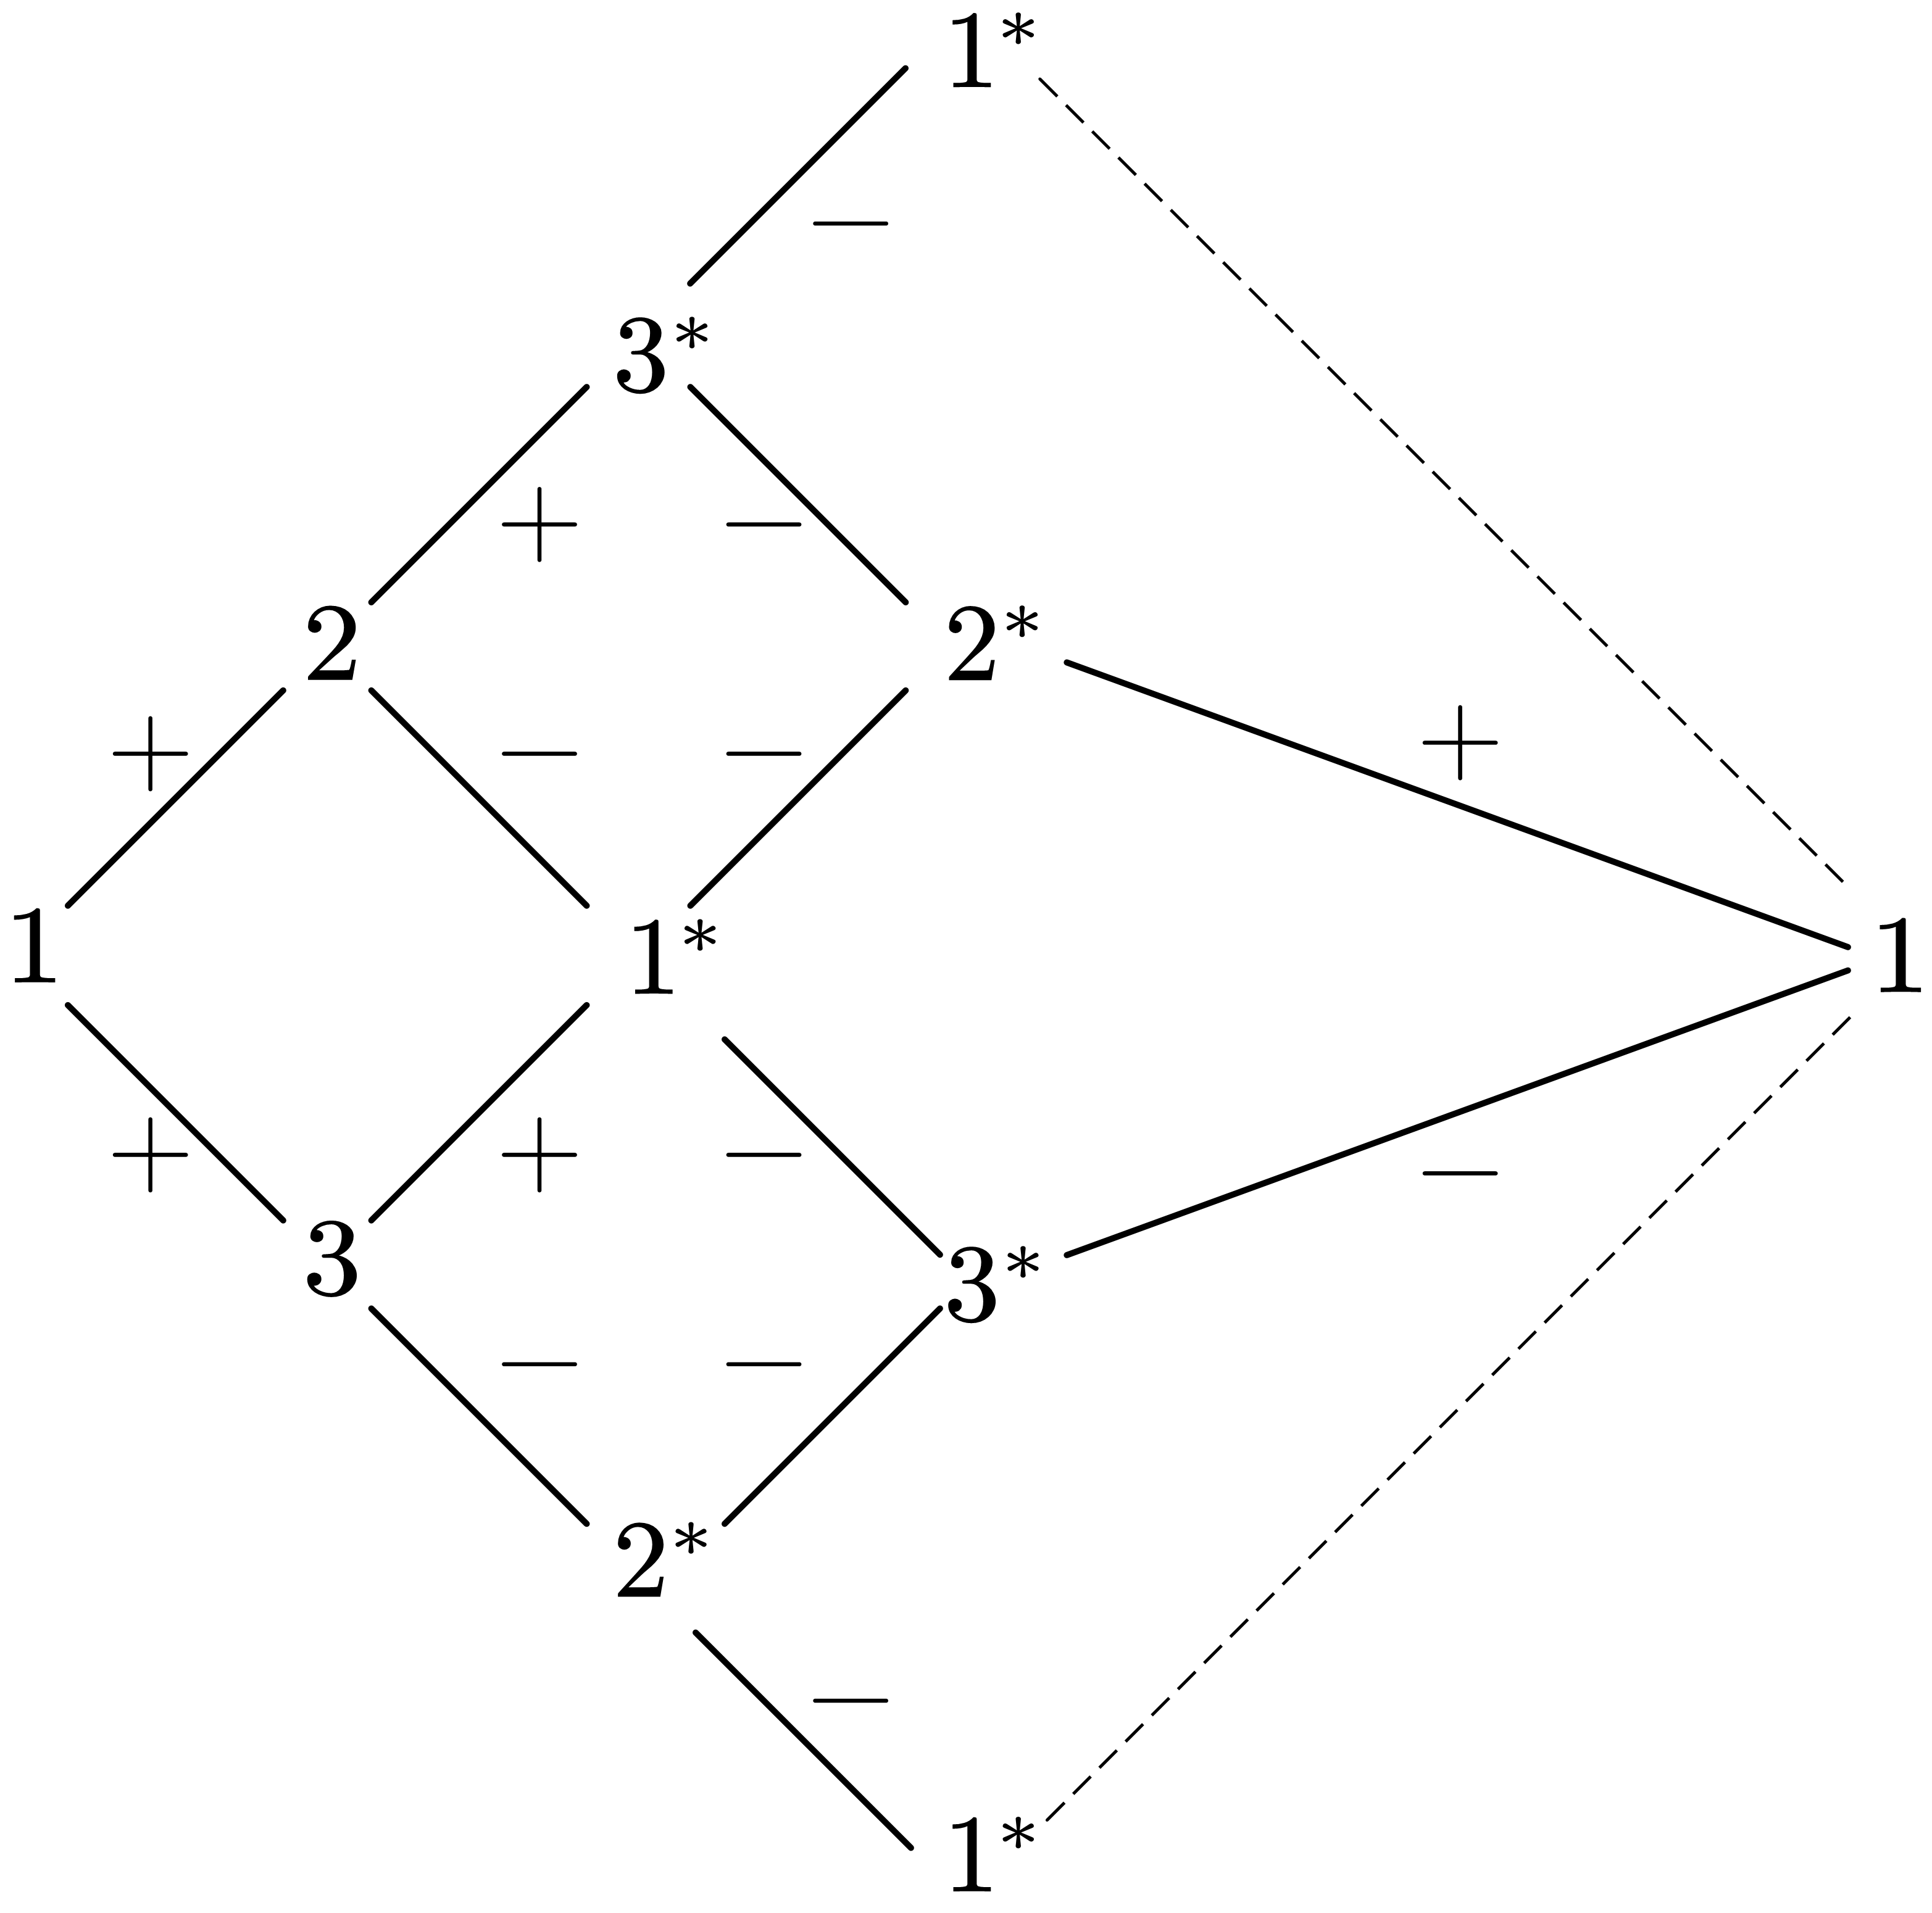
\includegraphics[scale=0.5,trim=0 -8 0 -8]{./pictures/6.07/pictorial_representation_1.png}
		\end{minipage} &
		
		\begin{minipage}{0.3\linewidth}
		\centering
		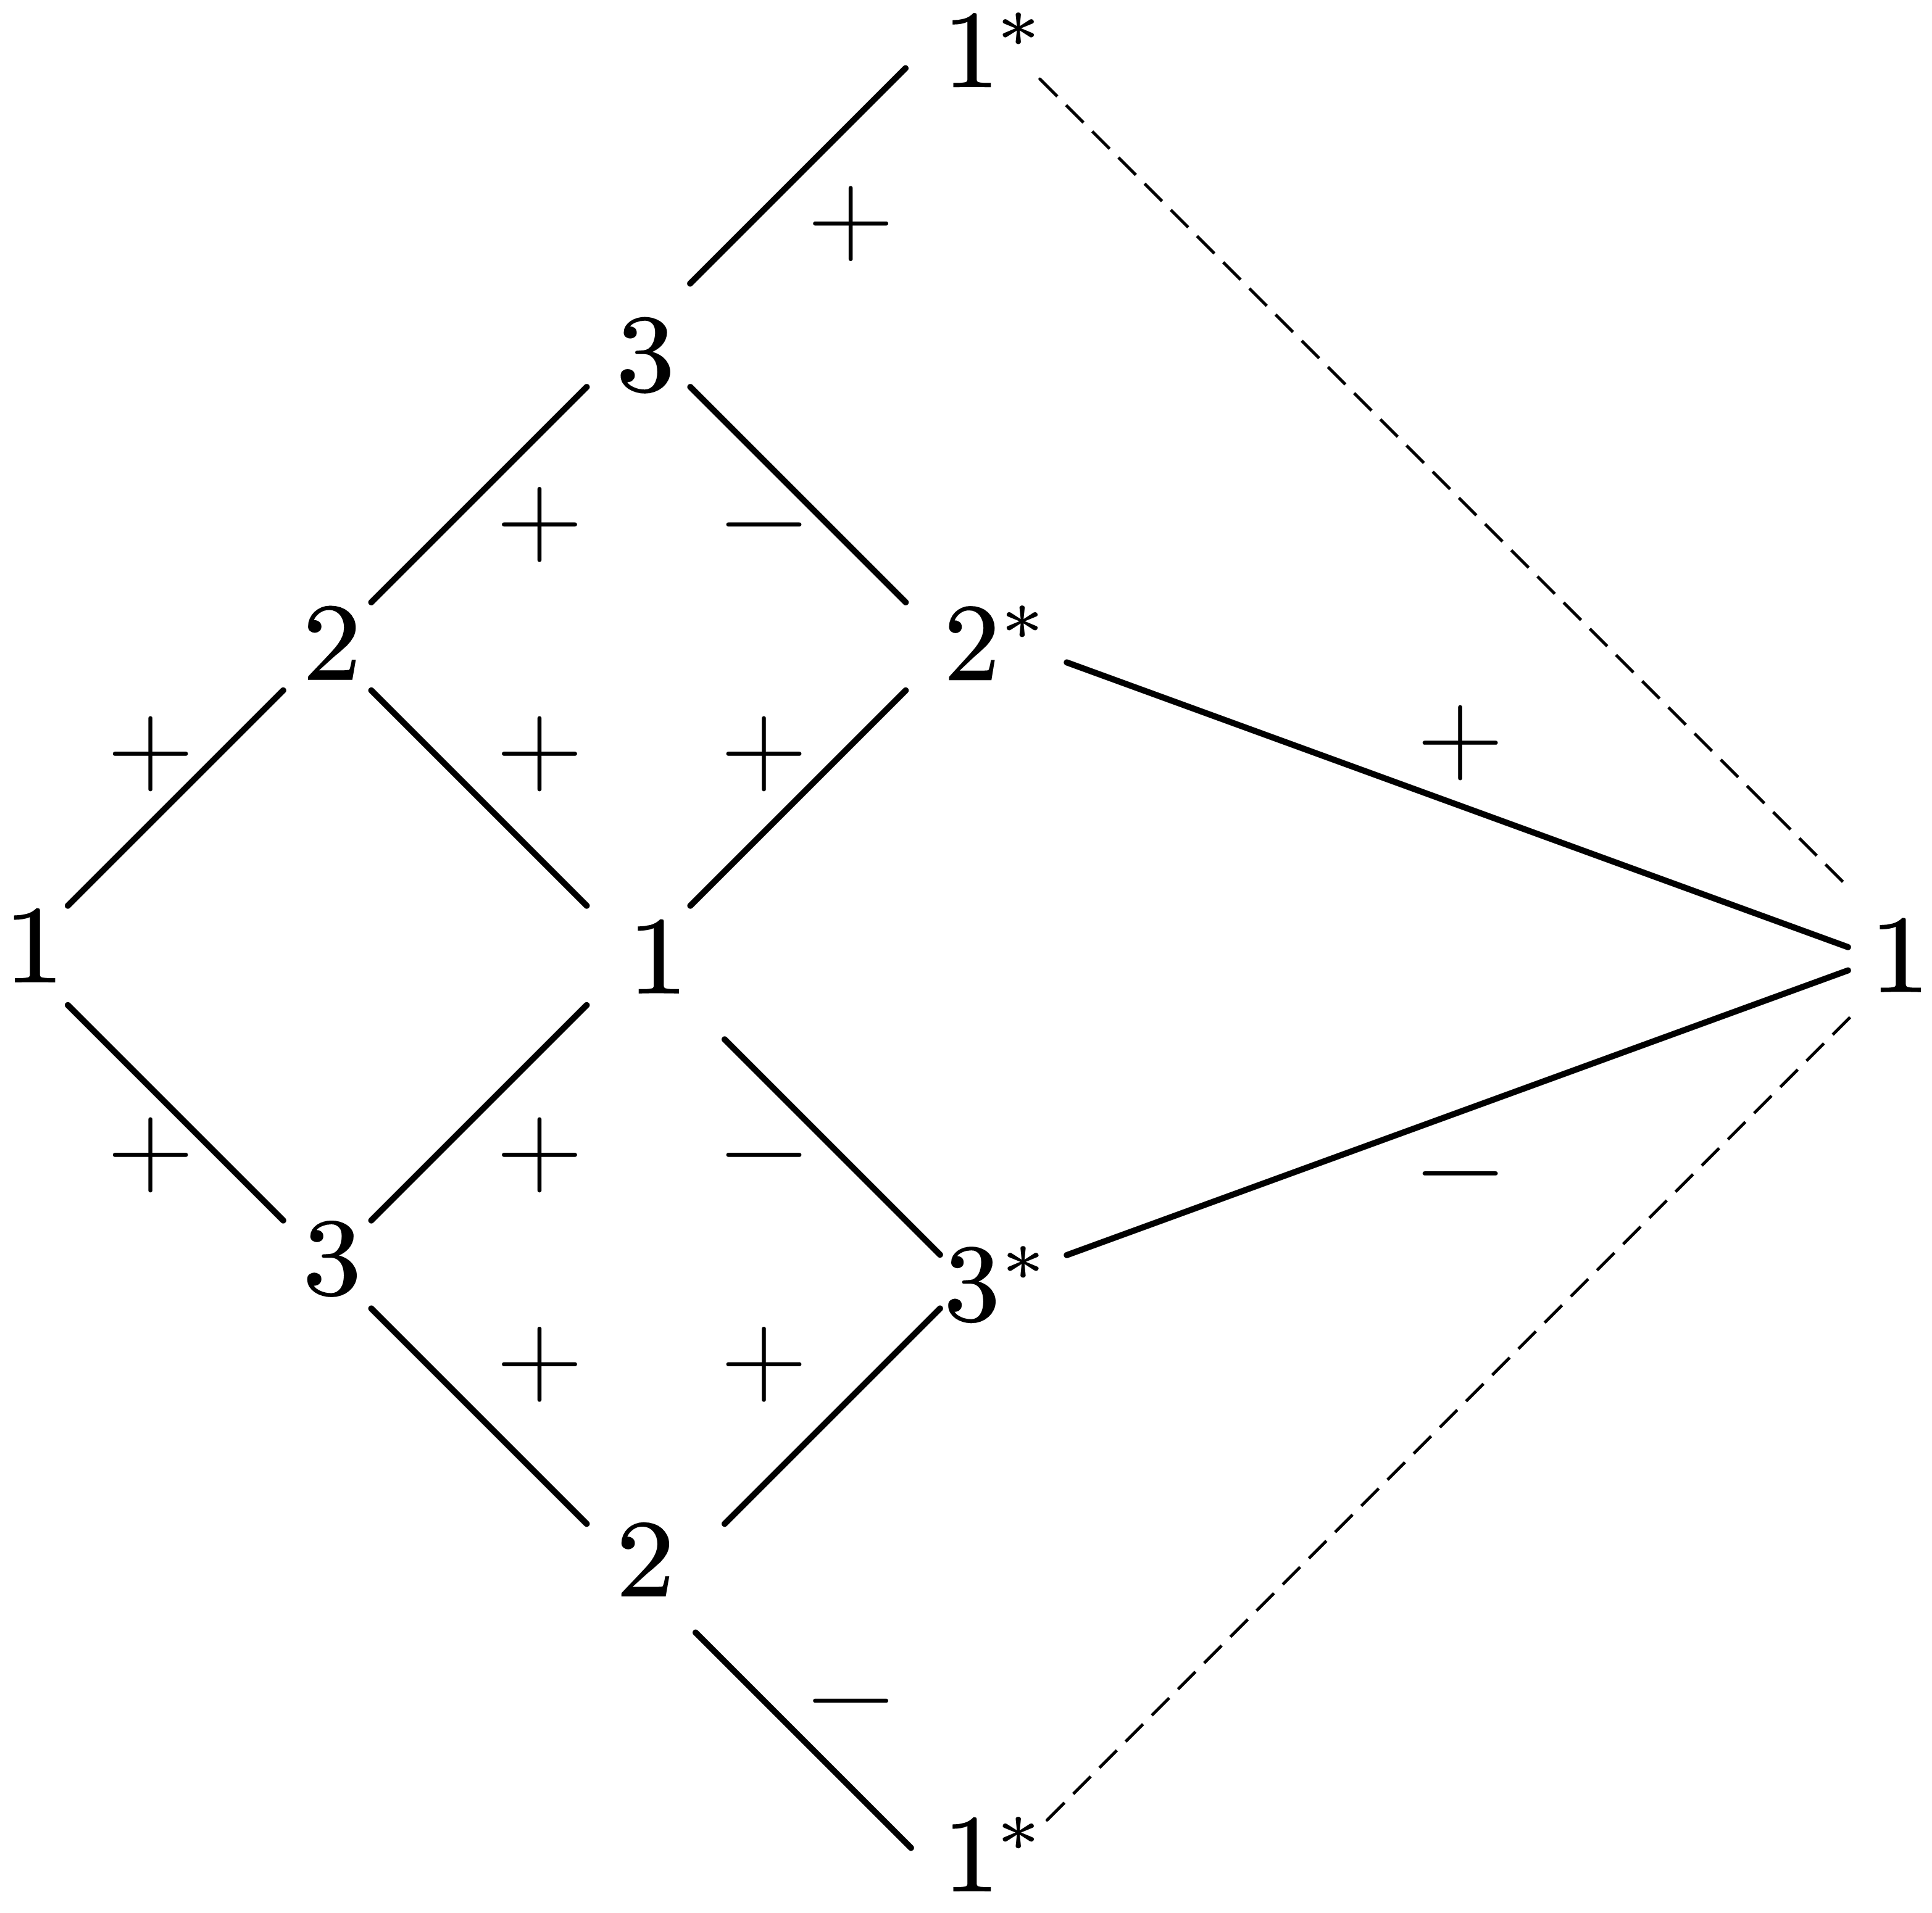
\includegraphics[scale=0.5,trim=0 -8 0 -8]{./pictures/6.07/pictorial_representation_2.png}
		\end{minipage} &
		
		\begin{minipage}{0.3\linewidth}
		\centering
		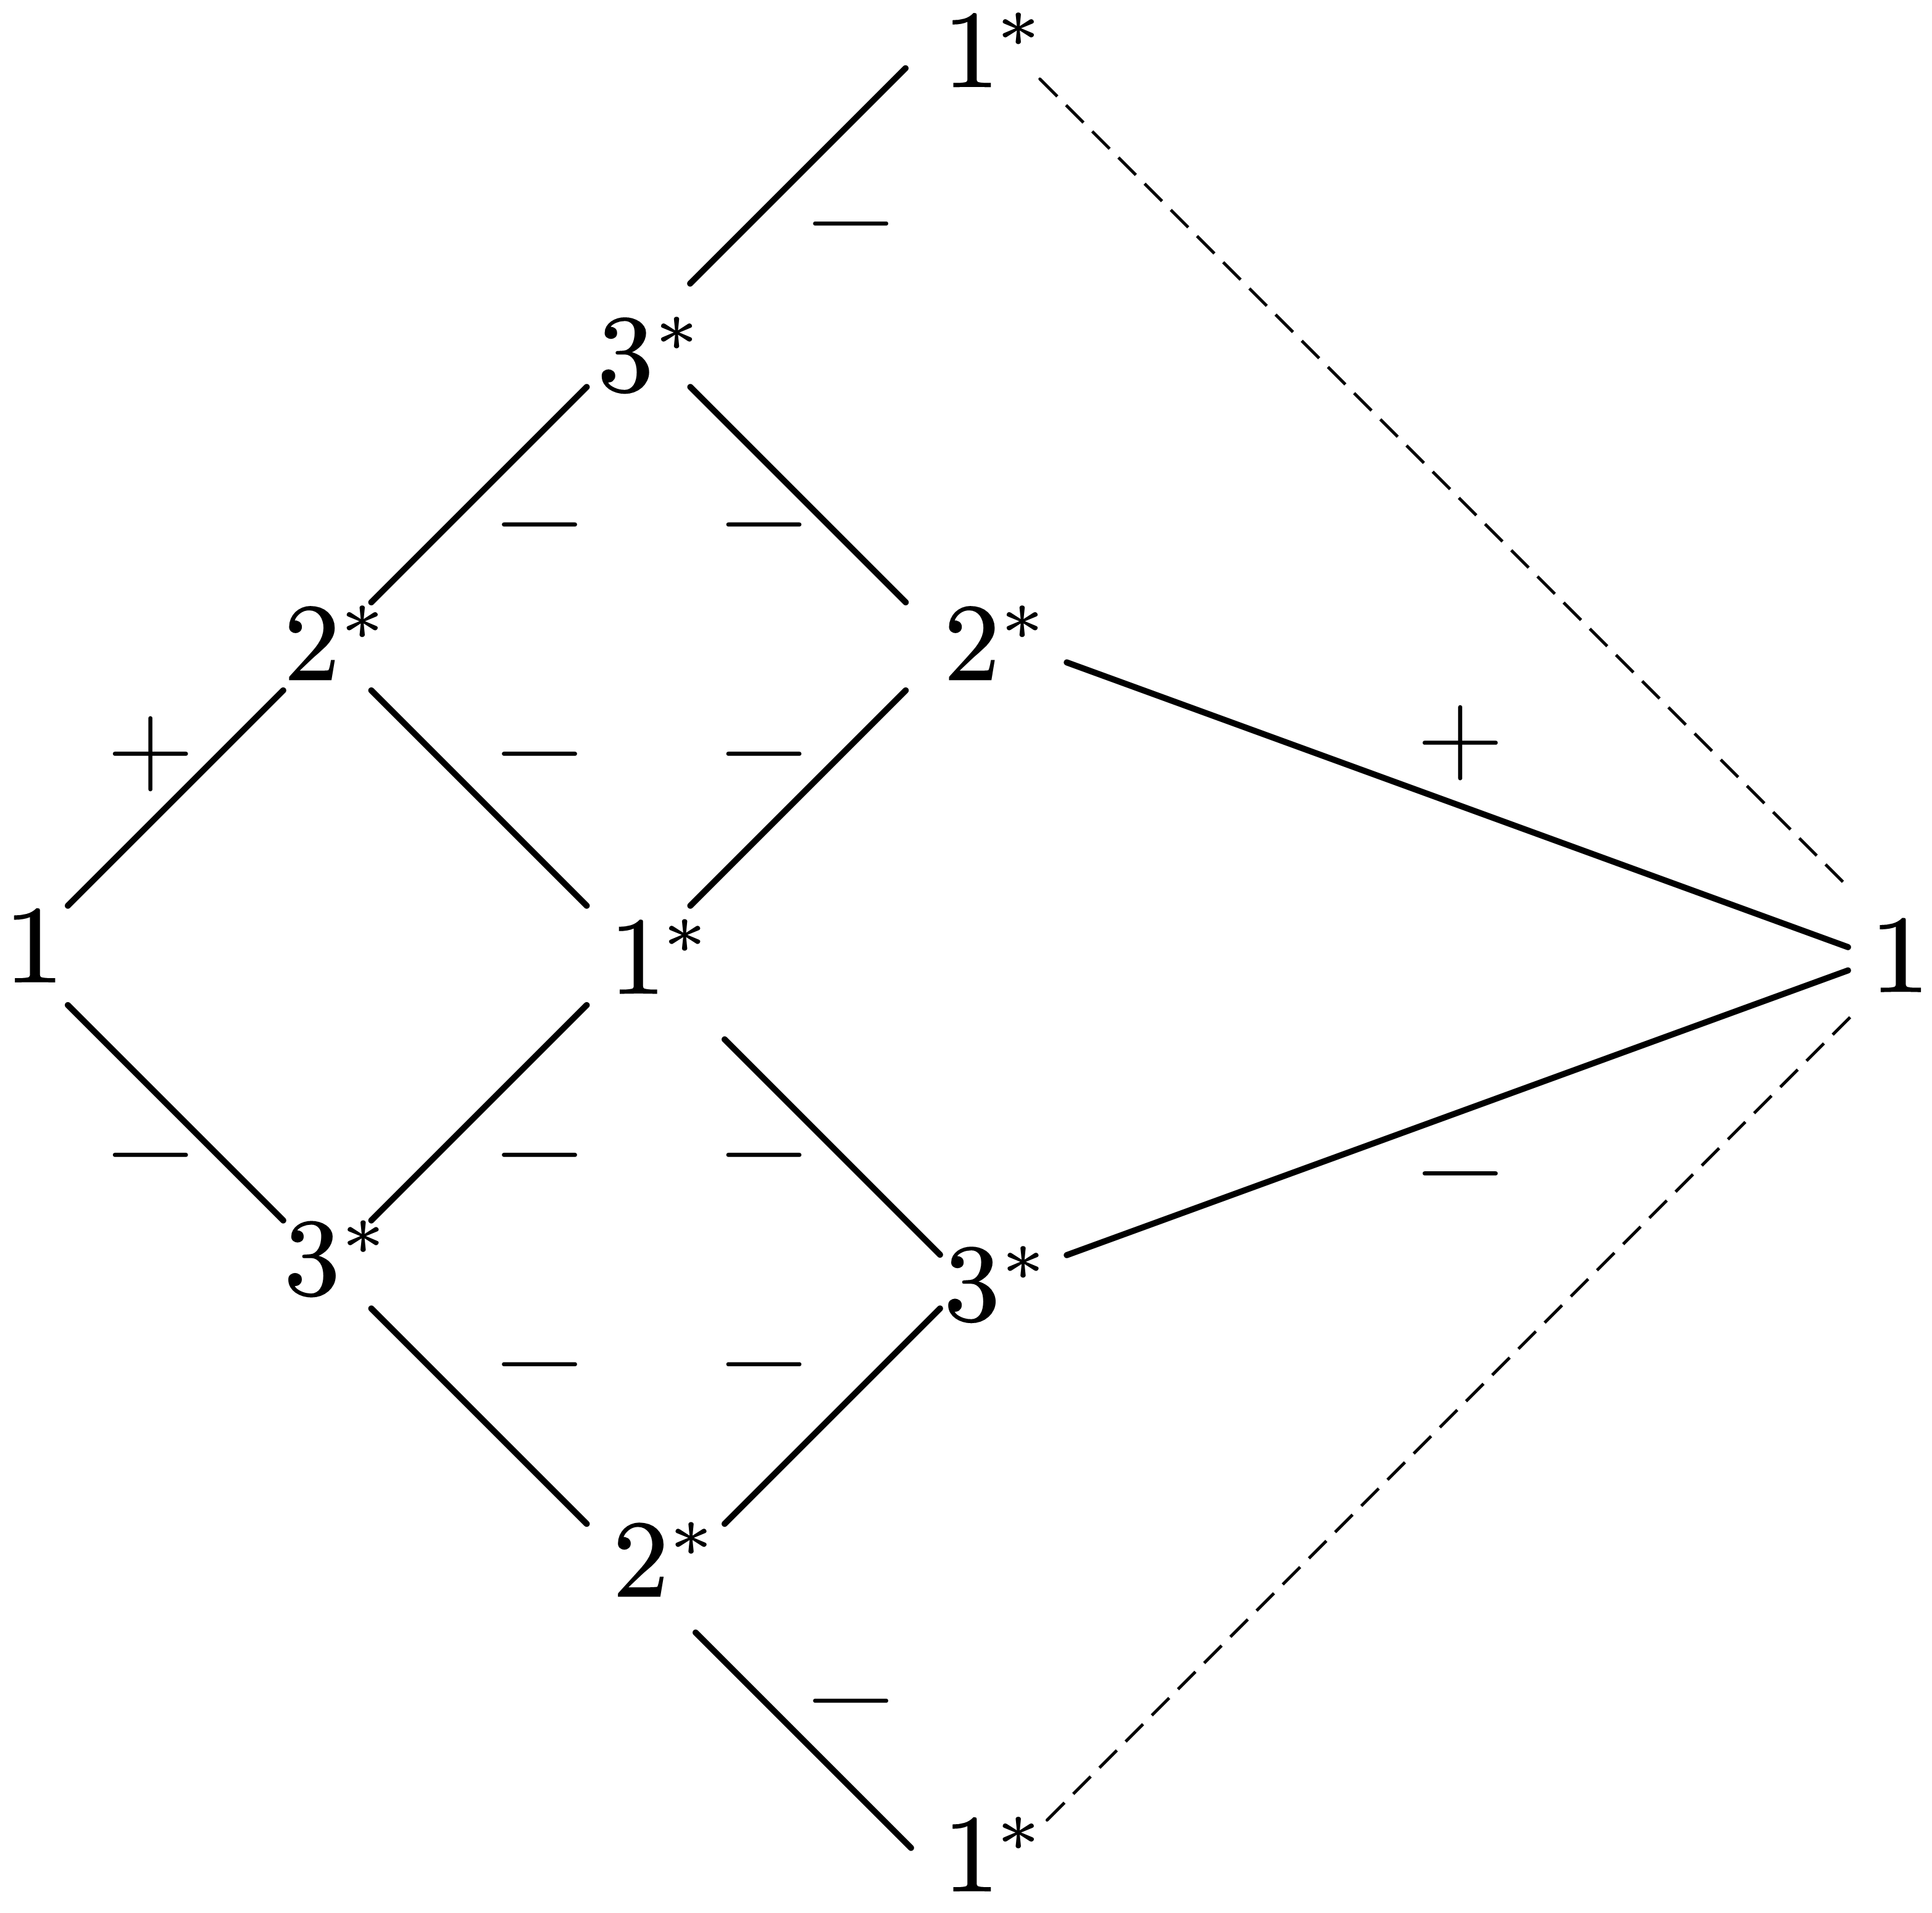
\includegraphics[scale=0.5,trim=0 -8 0 -8]{./pictures/6.07/pictorial_representation_3.png}
		\end{minipage} \\
		
		\begin{minipage}{0.3\linewidth}
		\centering
		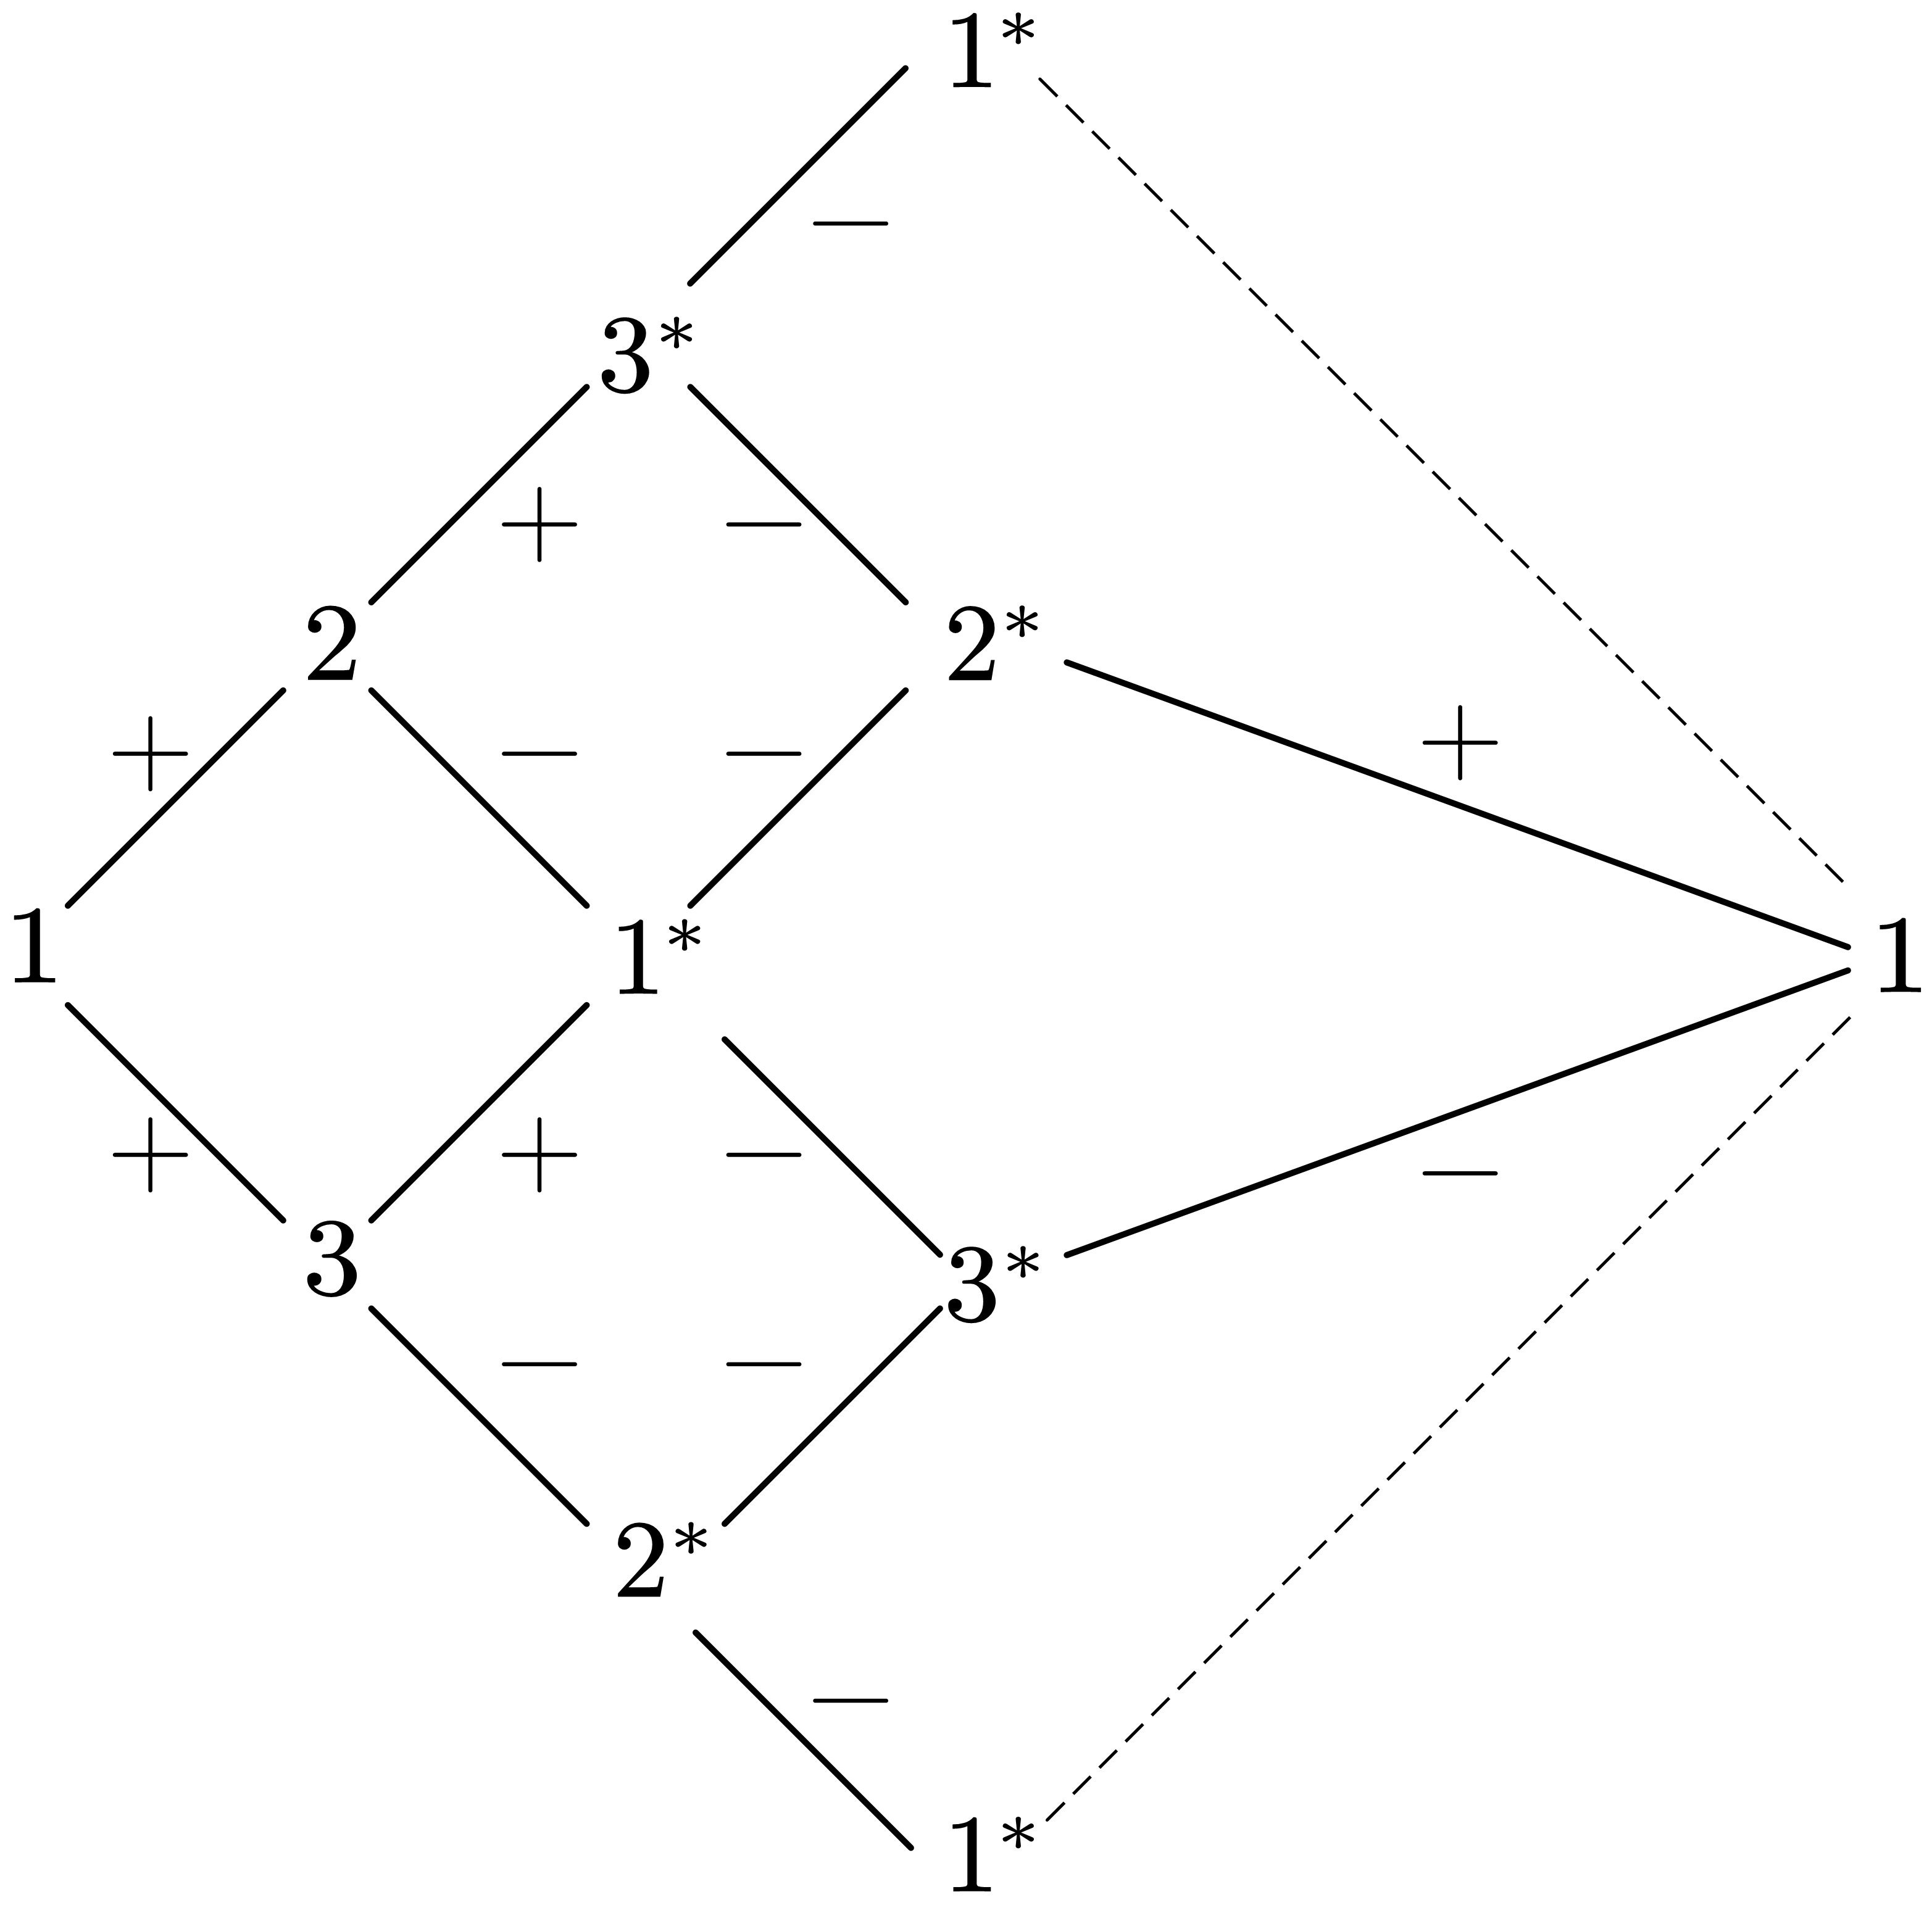
\includegraphics[scale=0.5,trim=0 -8 0 -8]{./pictures/6.07/pictorial_representation_4.png}
		\end{minipage} &
			
		\begin{minipage}{0.3\linewidth}
		\centering
		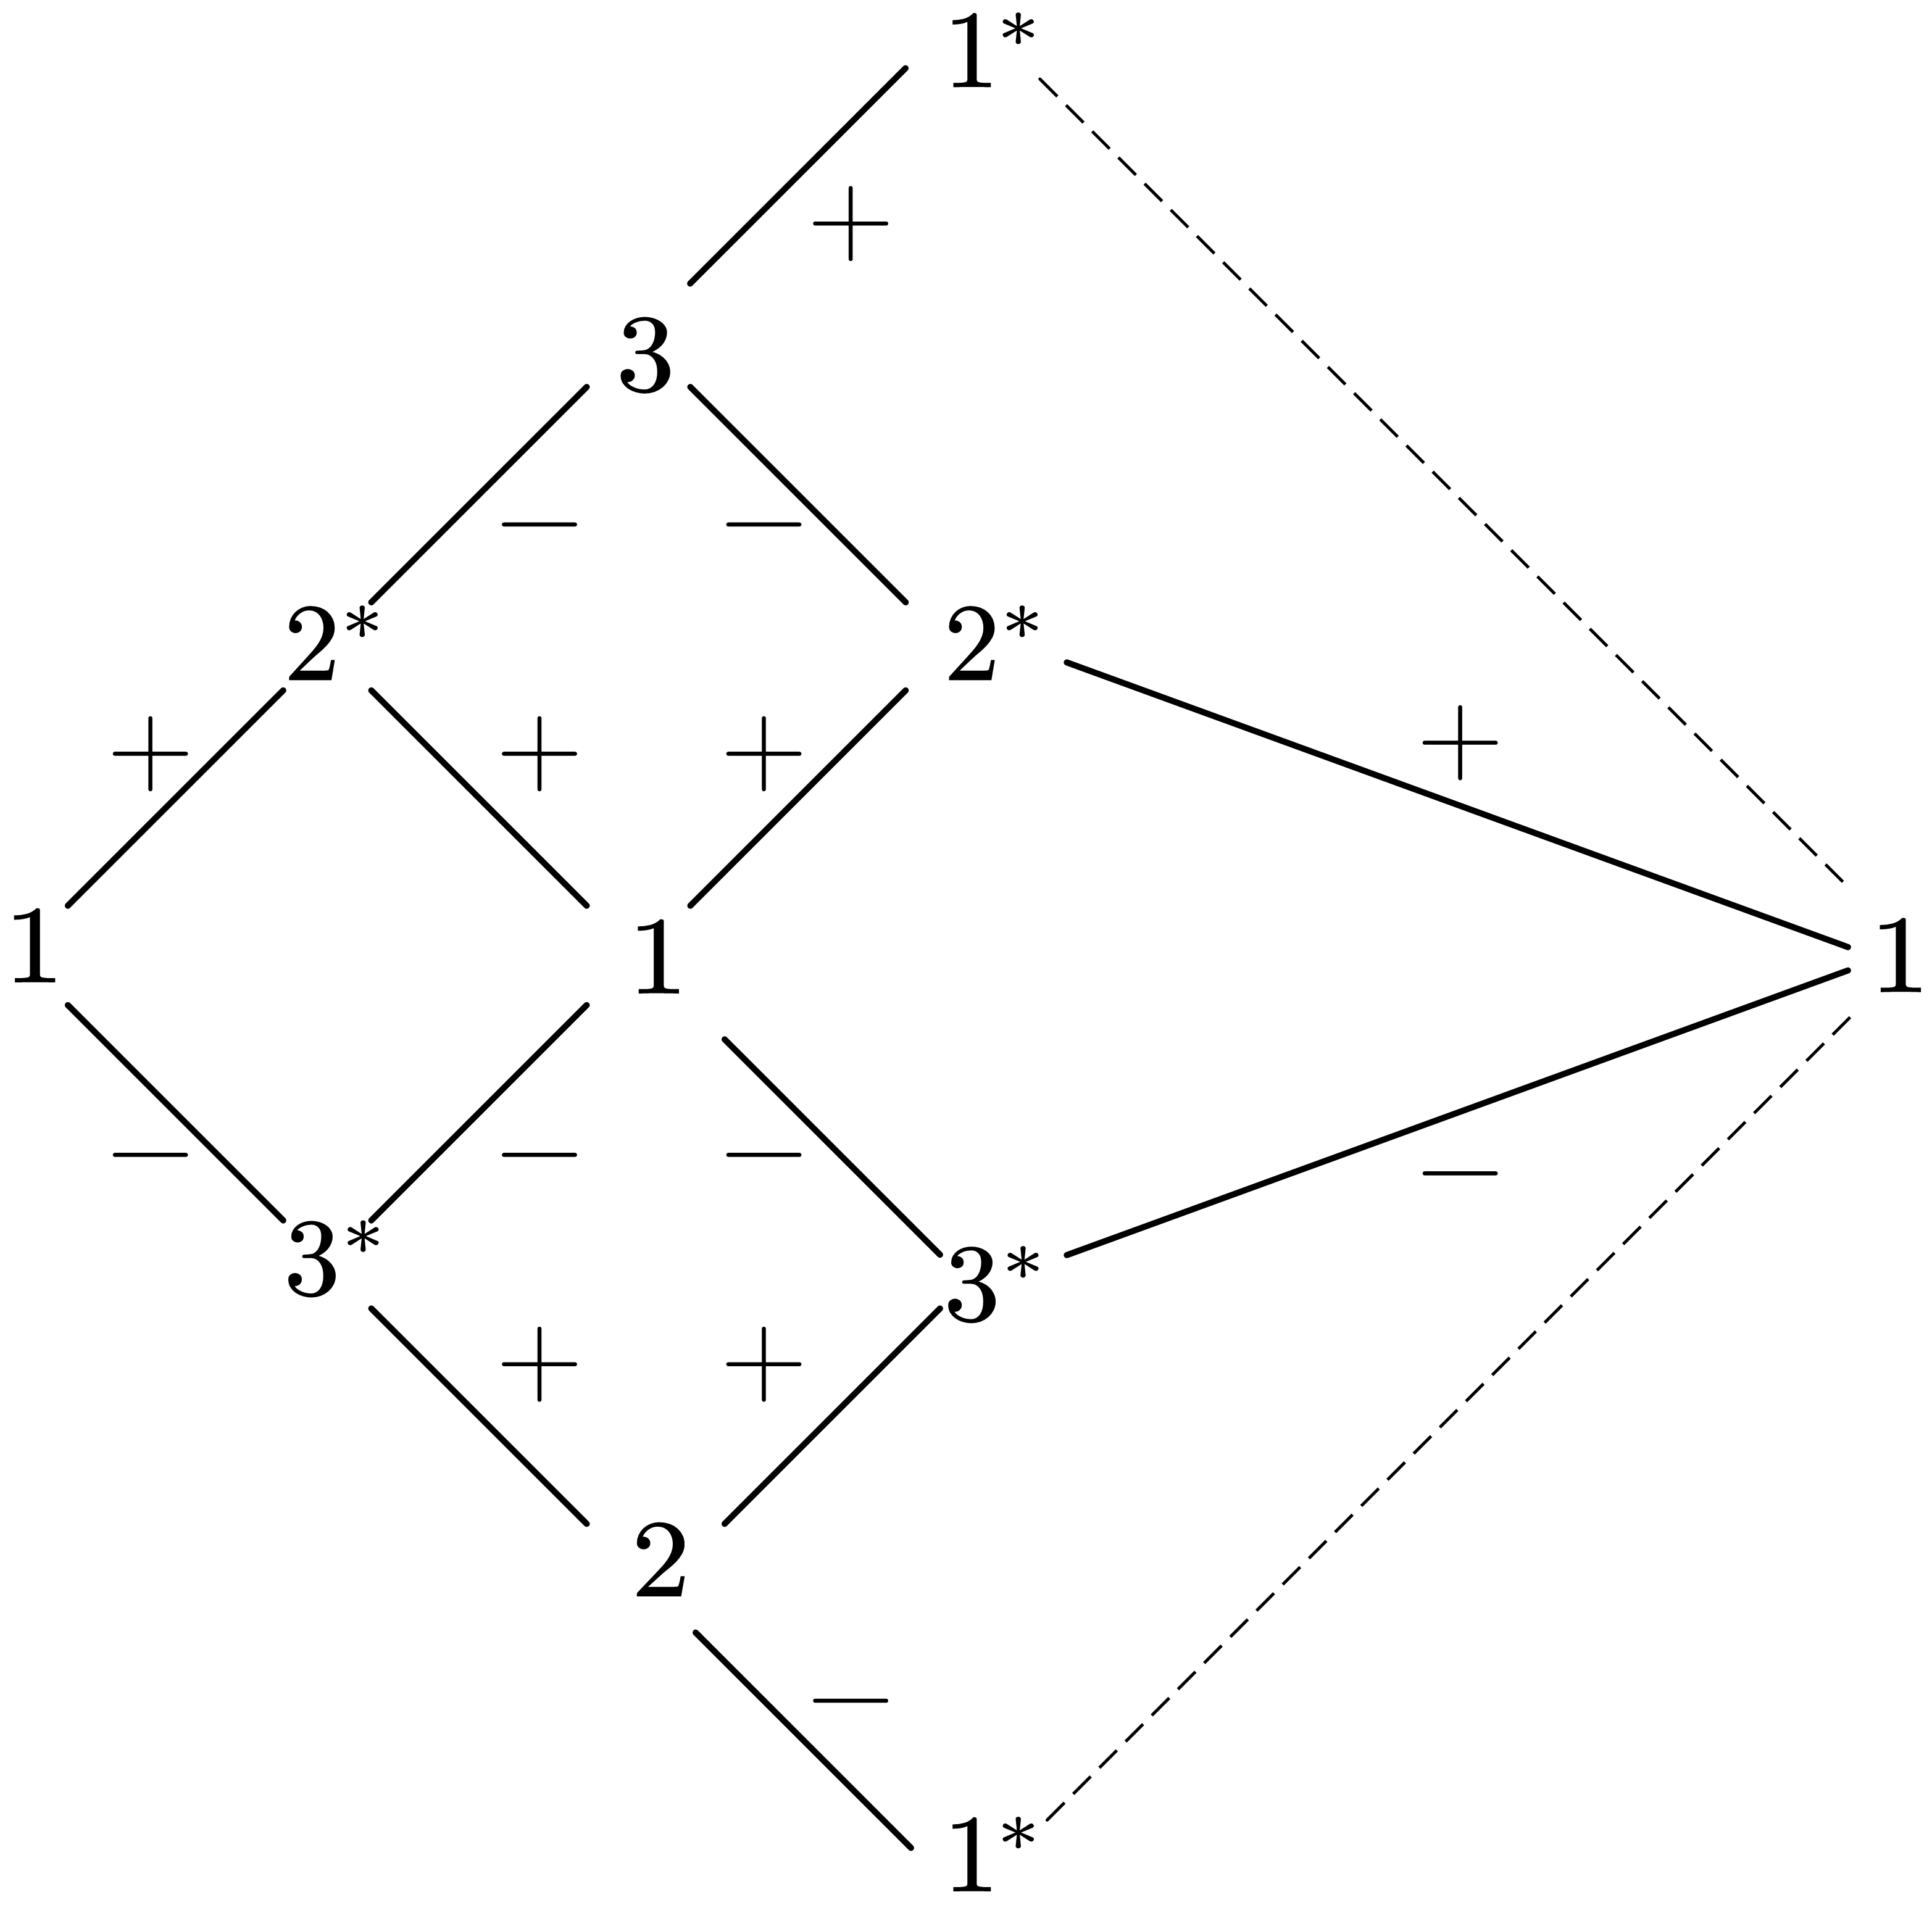
\includegraphics[scale=0.5,trim=0 -8 0 -8]{./pictures/6.07/pictorial_representation_5.png}
		\end{minipage} &
		
		\begin{minipage}{0.3\linewidth}
		\centering
		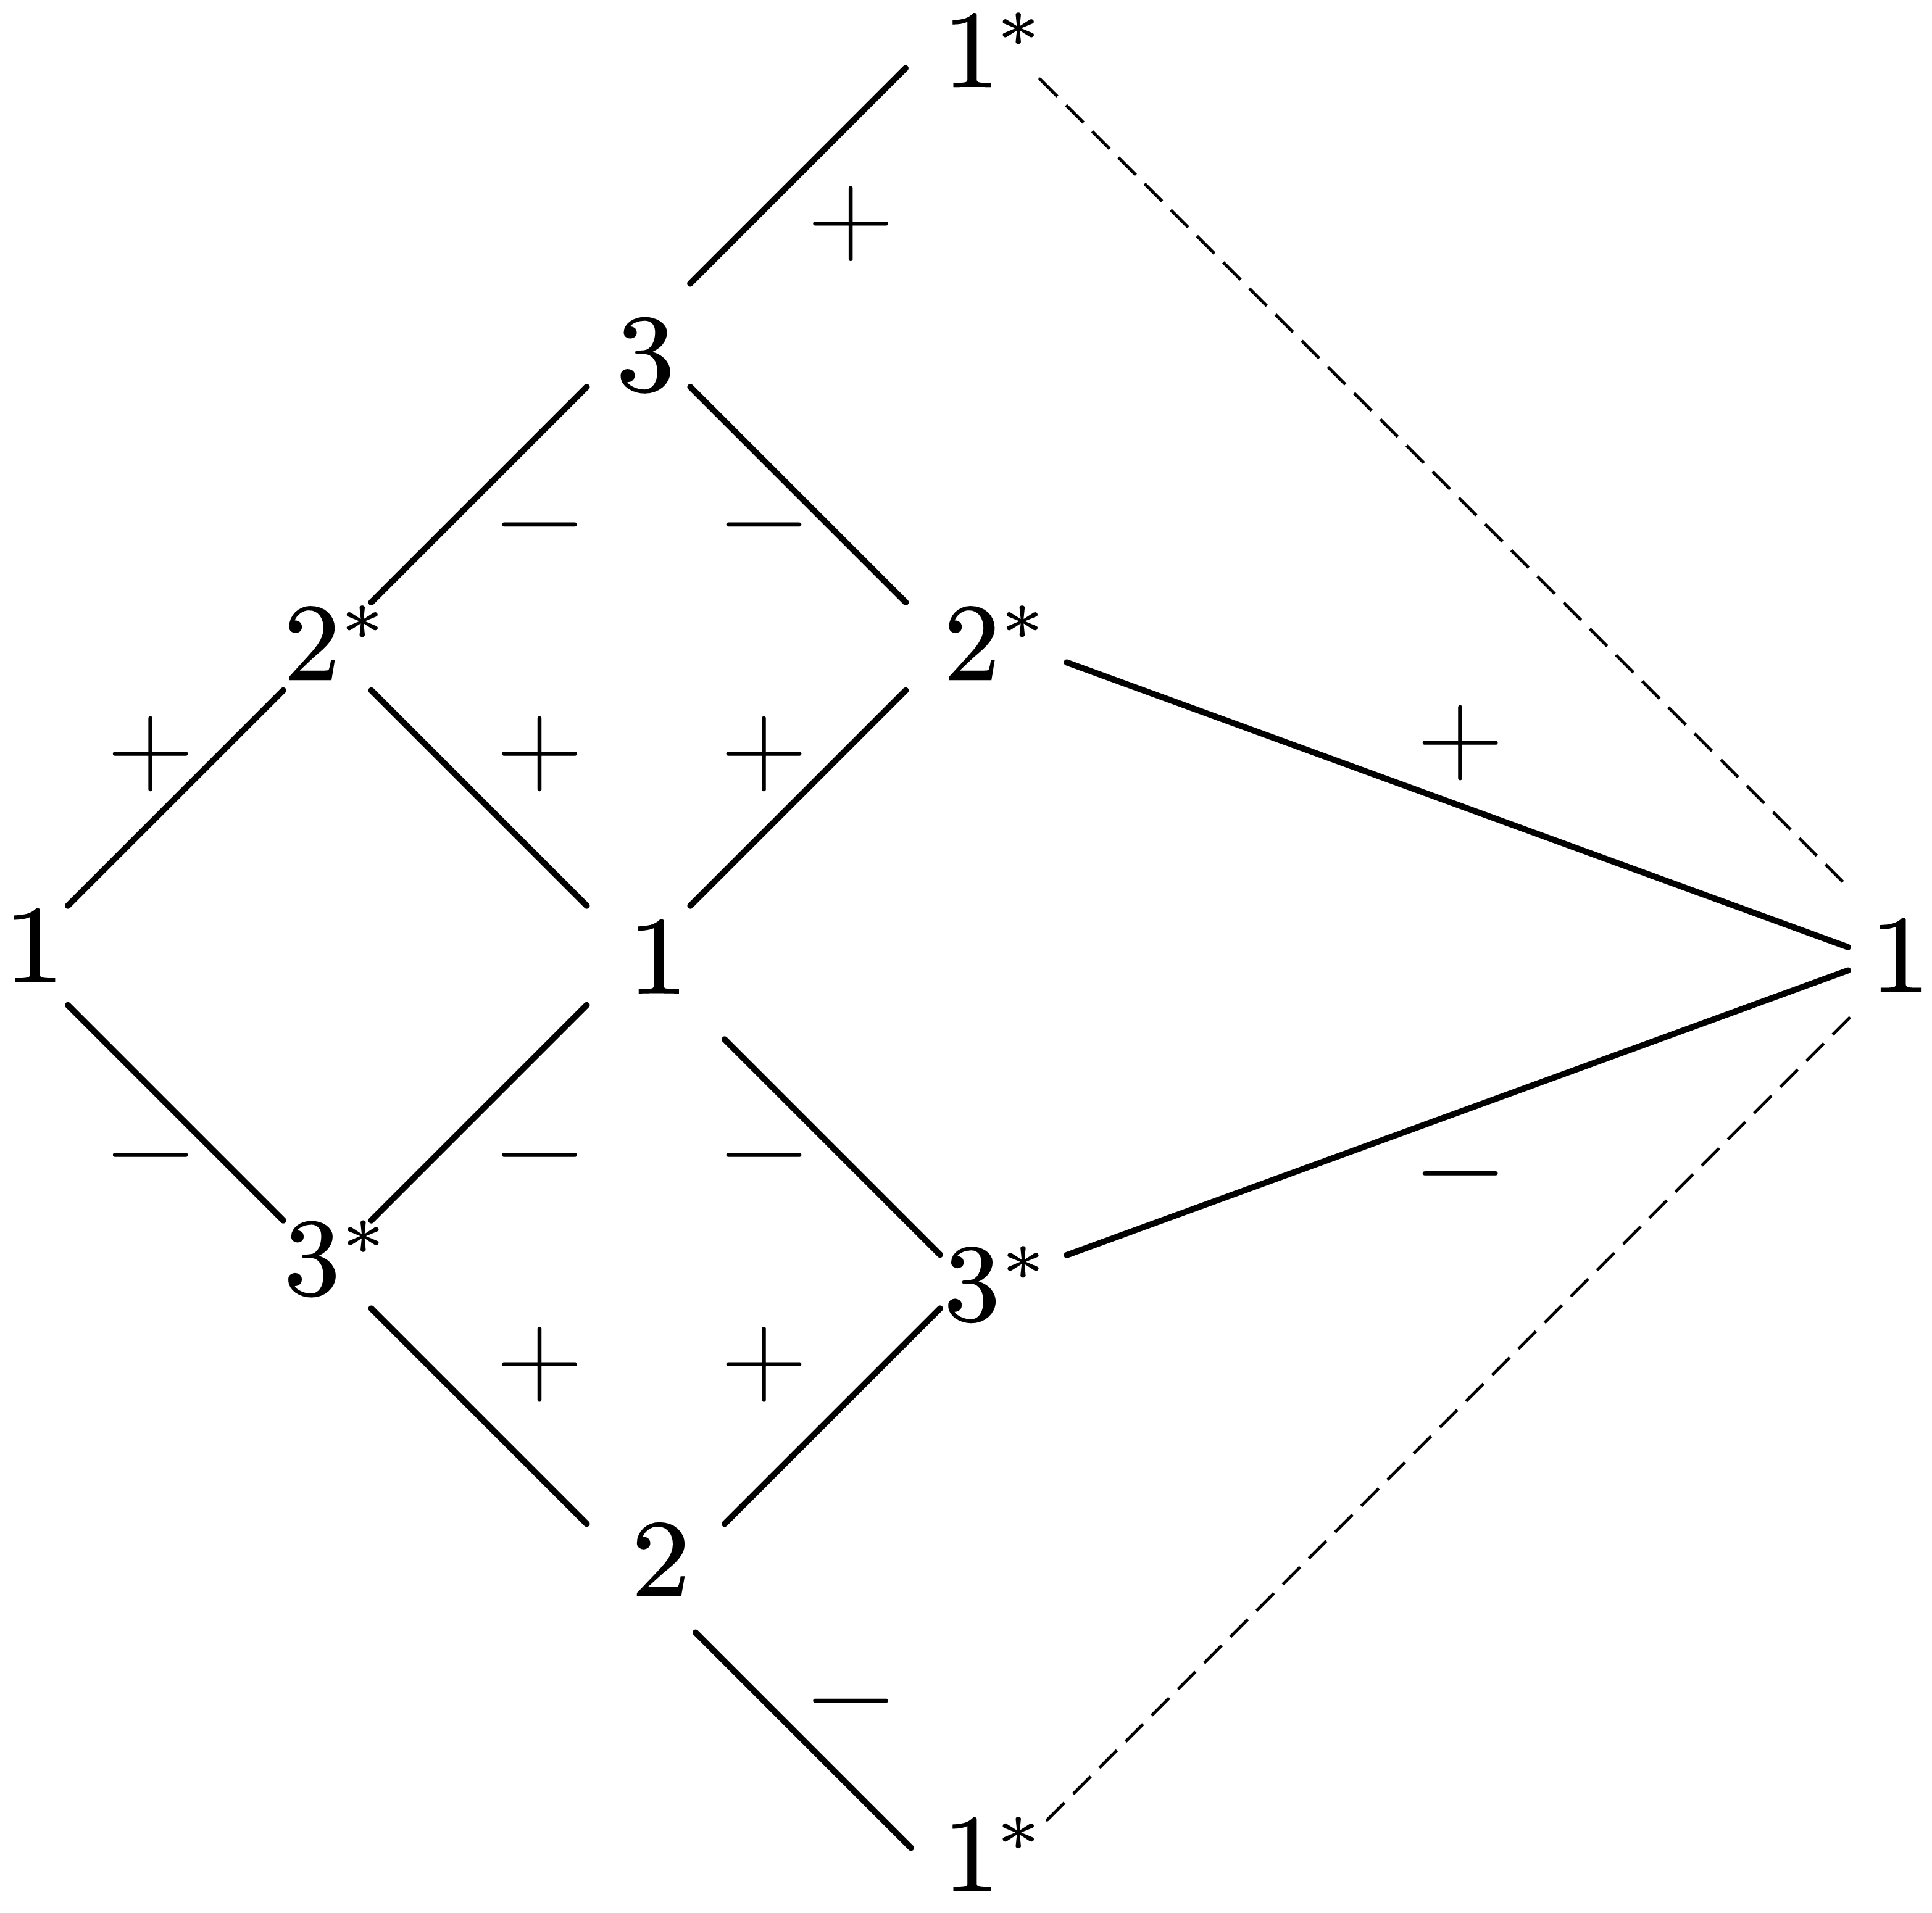
\includegraphics[scale=0.5,trim=0 -8 0 -8]{./pictures/6.07/pictorial_representation_6.png}
		\end{minipage}
		
	\end{tabular}
	\captionof{figure}{The pictorial representation of all fourth-order diagrams of the benzene.}\label{fig:exe7_2}
	\end{center}
	
	Now we will calculate all terms according to their pictorial representation. Instead of lengthy calculation, we only care about the path from 1 to 1 in each diagram. For example, for the first subdiagram of \Figref{fig:exe7_2}, we know that it has eight paths, six valid but two invalid. If a path has a segment with a plus/minus token, it will be marked as $+$/$-$, and zero otherwise. And thus, its eight paths are:
	\begin{center}
	\begin{tabular}{cccc}
		$(+,+,-,0)$ & $(+,+,-,+)$ & $(+,-,-,+)$ & $(+,-,-,-)$\\
		$(+,+,-,+)$ & $(+,+,-,-)$ & $(+,-,-,-)$ & $(+,-,-,0)$
	\end{tabular}
	\end{center}		
	If a path has a 0, the corresponding term is zero. Otherwise, the corresponding term has a factor $(-1)^k$, where $k$ is the number of its minus signs. Therefore, there are two positive and four negative terms, and the first term is
	\[
		(-1)^{2+1} \frac{2 \times 3}{ (2\beta)^3 } \left[ 2 \times \left( \frac{\beta^4}{16} \right) + 4 \times \left( -\frac{\beta^4}{16} \right) \right] = \frac{6}{64} \beta = \frac{N}{64} \beta,
	\]
	where the factor $2$ occurs for the closed-shell structure, and the factor $3$ is the number of occupied spin orbitals.
	
	Similarly, we find that the second, third, ..., sixth term is $\frac{N}{64} \beta$, $\frac{N}{64} \beta$, $\frac{N}{64} \beta$, $-\frac{3N}{128} \beta$, $-\frac{3N}{128} \beta$. Thus, we obtain that
	\begin{sequation}
		E^{(4)}_0 = 4 \times \left( \frac{N}{64} \beta \right) + 2 \times \left( -\frac{3N}{128} \beta \right) = \frac{N}{64} \beta.
	\end{sequation}

	\item[b.] As mentioned before, the general expression of the correlation energy with $N>6$ is also suitable for benzene. Thus, the correlation energy of the benzene is
	\begin{sequation}
		E^{(4)}_0({\rm benzene} ) = \frac{6}{64} \beta = \frac{3}{32} \beta,
	\end{sequation}		
	which agrees with the independently calculated result found in Exercise 6.6.
	
	\end{itemize}	
	
	\end{solution}
	
	\section{Perturbation Expansion of the Correlation Energy}
	
	% 6.8
	\begin{exercise}
	Derive Eqs.(6.73) and (6.74) starting with Eq.(6.72).
	\end{exercise}
	
	\begin{solution}

	The detailed simplification can be seen in Exercise 2.18.
	
	\end{solution}
	
	% 6.9
	\begin{exercise}
	Derive Eqs.(6.77) and (6.78) from Eq.(6.76).
	\end{exercise}
	
	\begin{solution}
	We assume that $\Delta \approx (\varepsilon_2 - \varepsilon_1)$, thus	
	\[
		\Delta = ( \varepsilon_2 - \varepsilon_1 ) + \frac{1}{2} J_{11} + \frac{1}{2} J_{22} - 2 J_{12} + K_{12} = ( \varepsilon_2 - \varepsilon_1 ) \left[ 1 + \frac{ J_{11} + J_{22} - 4 J_{12} + 2 K_{12} }{ 2 ( \varepsilon_2 - \varepsilon_1 ) } \right].
	\]
	Using binomial series and geometric series, we find that
	\begin{align*}
		E_\corr &= \Delta - \left( \Delta^2 + K^2_{12} \right)^{\frac{1}{2}} = \Delta \left[ 1 - \left( 1 + \frac{ K^2_{12} }{ \Delta^2 } \right)^{\frac{1}{2}} \right] = \Delta \left[ 1 - \left( 1 + \frac{ K^2_{12} }{ 2\Delta^2 } - \frac{ K^4_{12} }{ 8\Delta^4 } + \cdots \right) \right] \\
		&= - \frac{ K^2_{12} }{ 2\Delta } + \frac{ K^4_{12} }{ 8\Delta^3 } + \cdots \\
		&= - \frac{ K^2_{12} }{ 2( \varepsilon_2 - \varepsilon_1 ) \left[ 1 + \frac{ J_{11} + J_{22} - 4 J_{12} + 2 K_{12} }{ 2 ( \varepsilon_2 - \varepsilon_1 ) } \right] } + \frac{ K^4_{12} }{ 8 ( \varepsilon_2 - \varepsilon_1 )^3 \left[ 1 + \frac{ J_{11} + J_{22} - 4 J_{12} + 2 K_{12} }{ 2 ( \varepsilon_2 - \varepsilon_1 ) } \right]^3 } + \cdots \\
		&= - \frac{ K^2_{12} }{ 2( \varepsilon_2 - \varepsilon_1 )} \left[ 1 - \frac{ J_{11} + J_{22} - 4 J_{12} + 2 K_{12} }{ 2 ( \varepsilon_2 - \varepsilon_1 ) } + \left( \frac{ J_{11} + J_{22} - 4 J_{12} + 2 K_{12} }{ 2 ( \varepsilon_2 - \varepsilon_1 ) } \right)^2 + \cdots \right] + \cdots \\
		&= - \frac{ K^2_{12} }{ 2( \varepsilon_2 - \varepsilon_1 )} + \frac{ K^2_{12} ( J_{11} + J_{22} - 4 J_{12} + 2 K_{12} ) }{ 4( \varepsilon_2 - \varepsilon_1 )^2 } + o\left( \left( \frac{1}{ \varepsilon_2 - \varepsilon_1 } \right)^2 \right) .
	\end{align*}
	Thus, we obtain (6.77) and (6.78) from (6.76).
	
	\end{solution}
	
	\section{The \texorpdfstring{$N$}--Dependence of the RS Perturbation Expansion}
	
	% 6.10
	\begin{exercise}
	Derive Eqs.(6.80b) and (6.90).
	\end{exercise}
	
	\begin{solution}
	From (6.68), we find that with the truth that all two-electron integrals involving orbitals from different units are zero and $\langle mm || mm \rangle = 0$,
	\begin{align*}
		E^{(1)}_0 &= - \frac{1}{2} \sum_{ i=1 }^{2N} \sum_{ j=1 }^{2N} \langle 1_i 1_j || 1_i 1_j \rangle = - \frac{1}{2} \sum_{ i=1 }^{2N} \langle 1_i 1_i || 1_i 1_i \rangle \\
			&= - \frac{1}{2} \sum_{ i=1 }^N \langle 1_i 1_i || 1_i 1_i \rangle + \langle 1_i \bar{1}_i || 1_i \bar{1}_i \rangle + \langle \bar{1}_i 1_i || \bar{1}_i 1_i \rangle + \langle \bar{1}_i \bar{1}_i || \bar{1}_i \bar{1}_i \rangle = -\frac{1}{2} \sum_{ i=1 }^N 2J_{11} = -\sum_{ i=1 }^N J_{11} = -N J_{11}.
	\end{align*}
	
	Besides, we obtain that
	\begin{align*}
		\langle \Psi^{2_i \bar{2}_i}_{1_i \bar{1}_i} | \mathscr{V} | \Psi^{2_i \bar{2}_i}_{1_i \bar{1}_i} \rangle &= \langle \Psi^{2_i \bar{2}_i}_{1_i \bar{1}_i} | \mathscr{H} | \Psi^{2_i \bar{2}_i}_{1_i \bar{1}_i} \rangle - \langle \Psi^{2_i \bar{2}_i}_{1_i \bar{1}_i} | \mathscr{H}_0 | \Psi^{2_i \bar{2}_i}_{1_i \bar{1}_i} \rangle \\
		&= \sum_{ i=1 }^{2N} h_{11} + 2h_{22} - 2h_{11} + \sum_{ i=1 }^N  J_{11} + J_{22} - J_{11} - \left[ ( 2N - 2 ) \varepsilon_1 + 2\varepsilon_2 \right] \\
		&= (2N-2)h_{11} + 2h_{22} + (N-1) J_{11} + J_{22} - (2N-2) ( h_{11} + J_{11} ) - 2 (h_{22} + 2J_{12} - K_{12})\\
		&= -(N-1) J_{11} + J_{22} - 4J_{12} + 2K_{12}. 
	\end{align*}
	
	\end{solution}
	
	\sectionstar{Diagrammatic Representation of the Perturbation Expansion of the Correlation Energy}
	
	\subsection{Hugenholtz Diagrams}
	
	% 6.11
	\begin{exercise}
	Show that the fourth-order diagram
	
	\begin{center}
	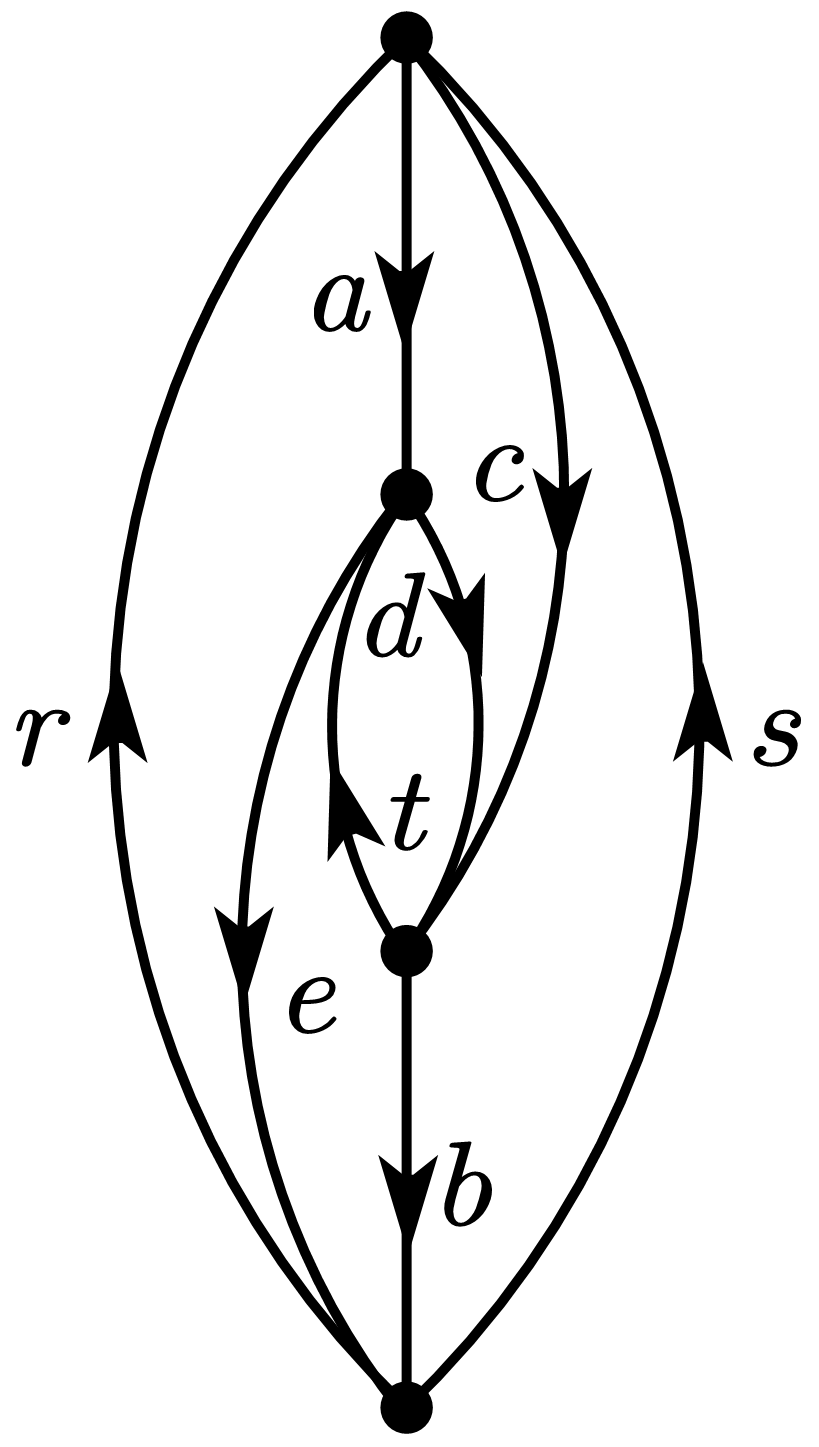
\includegraphics[scale=0.9]{./pictures/6.11/exercise.png}
	\end{center}
	is equal to
	\[
		-\frac{1}{2} \sum_{abcderst} \frac{ \langle rs || ac \rangle \langle at || de \rangle \langle dc || tb \rangle \langle eb||rs \rangle }{ ( \varepsilon_a + \varepsilon_c - \varepsilon_r - \varepsilon_s ) ( \varepsilon_c + \varepsilon_d + \varepsilon_e - \varepsilon_r - \varepsilon_t - \varepsilon_s ) ( \varepsilon_b + \varepsilon_e - \varepsilon_r - \varepsilon_s ) }.
	\]	
	
	\end{exercise}
	
	\begin{solution}
	
	Using the diagrammatic method, this term is made of four parts as follows.
	\begin{enumerate}
	
	\item There are 5 hole lines ($a$, $b$, $c$, $d$, $e$) and 3 particle lines ($r$, $s$, $t$). Thus we add a summation token with subscripts $abcderst$. 
	
	\item There are 2 loops, $r \rightarrow a \rightarrow d \rightarrow t \rightarrow e \rightarrow r$, $s \rightarrow c \rightarrow b \rightarrow s$, and 5 hole lines, thus we should add a $(-1)^{2+5} = (-1)^7$.	
	
	\item From the top to the bottom, 4 dots contribute $\langle rs|| ac \rangle$, $\langle at||de \rangle$, $\langle dc || tb \rangle$, $\langle eb || rs \rangle$, respectively.
	
	\item There are 3 imaginary horizontal lines.
		\begin{itemize}
		
		\item The first one crosses $a$, $c$, $r$, $s$, contributing a factor $\varepsilon_a + \varepsilon_c - \varepsilon_r - \varepsilon_s$ to the denominator.
		
		\item The second one crosses $c$, $d$, $e$, $r$, $t$, $s$ contributing a factor $\varepsilon_c + \varepsilon_d + \varepsilon_e - \varepsilon_r - \varepsilon_t - \varepsilon_s$ to the denominator.
		
		\item The third one crosses $b$, $e$, $r$, $s$, contributing a factor $\varepsilon_b + \varepsilon_e - \varepsilon_r - \varepsilon_s$ to the denominator.
		
		\end{itemize}			
	
	\end{enumerate}
	
	In conclusion, we know the mathematical expression of this diagram is
	\begin{sequation}
		-\frac{1}{2} \sum_{abcderst} \frac{ \langle rs || ac \rangle \langle at || de \rangle \langle dc || tb \rangle \langle eb||rs \rangle }{ ( \varepsilon_a + \varepsilon_c - \varepsilon_r - \varepsilon_s ) ( \varepsilon_c + \varepsilon_d + \varepsilon_e - \varepsilon_r - \varepsilon_t - \varepsilon_s ) ( \varepsilon_b + \varepsilon_e - \varepsilon_r - \varepsilon_s ) }.
	\end{sequation}
	
	\end{solution}
	
	\subsection{Goldstone Diagrams}
	
	% 6.12
	\begin{exercise}
	We stated that the Goldstone diagrams in Table 6.2 can be obtained by ``pulling apart" the second- and third-order Hugenholtz diagrams. This is quite tricky to see but the converse is much easier. For example, if we push
	
	\begin{center}
	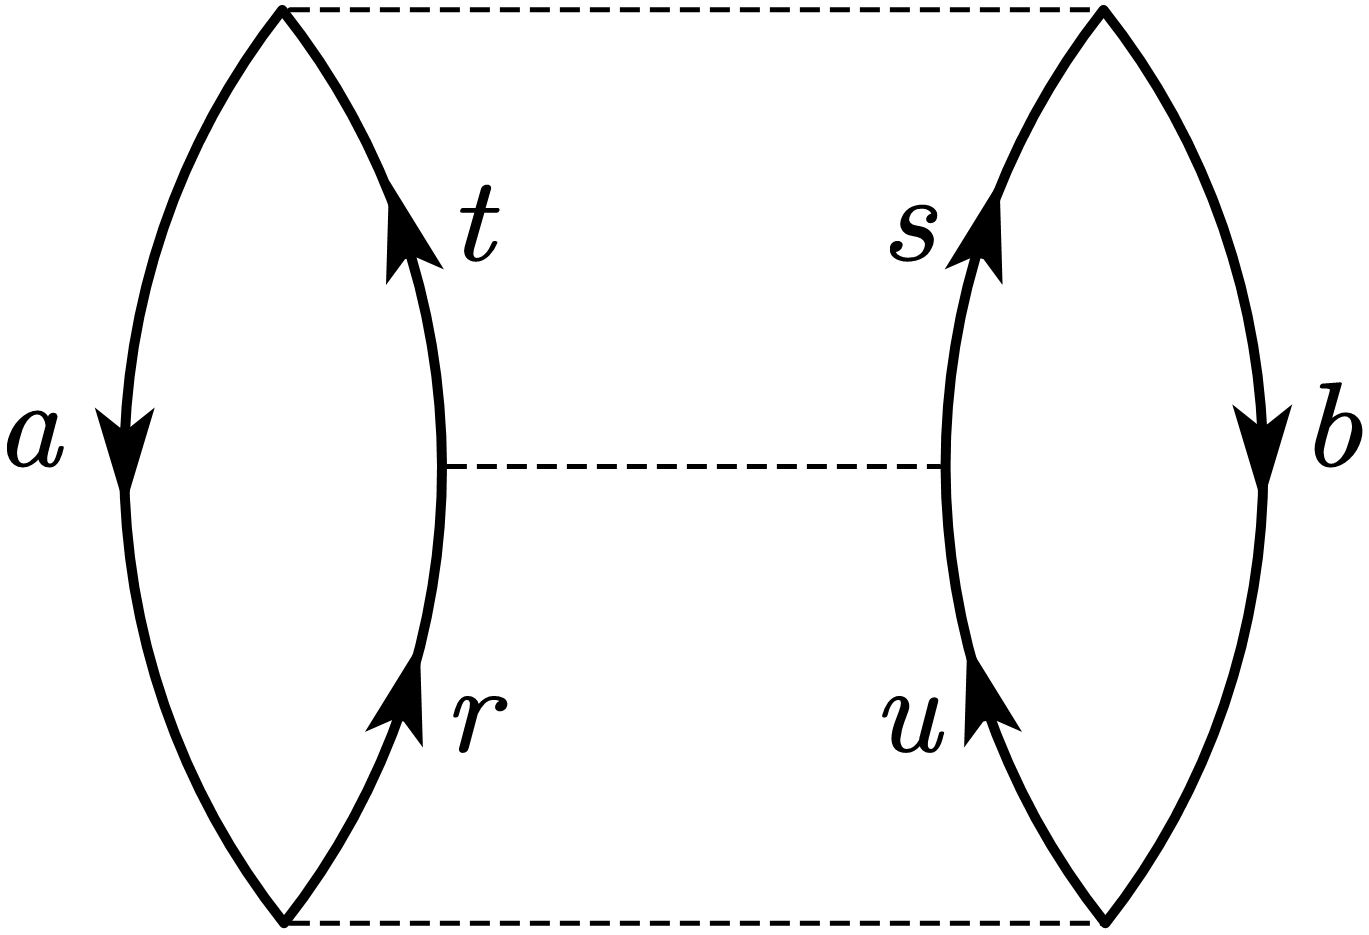
\includegraphics[scale=0.9]{./pictures/6.12/exercise_1.png}
	\end{center}
	
	together, it is clear that we obtain
	
	\begin{center}
	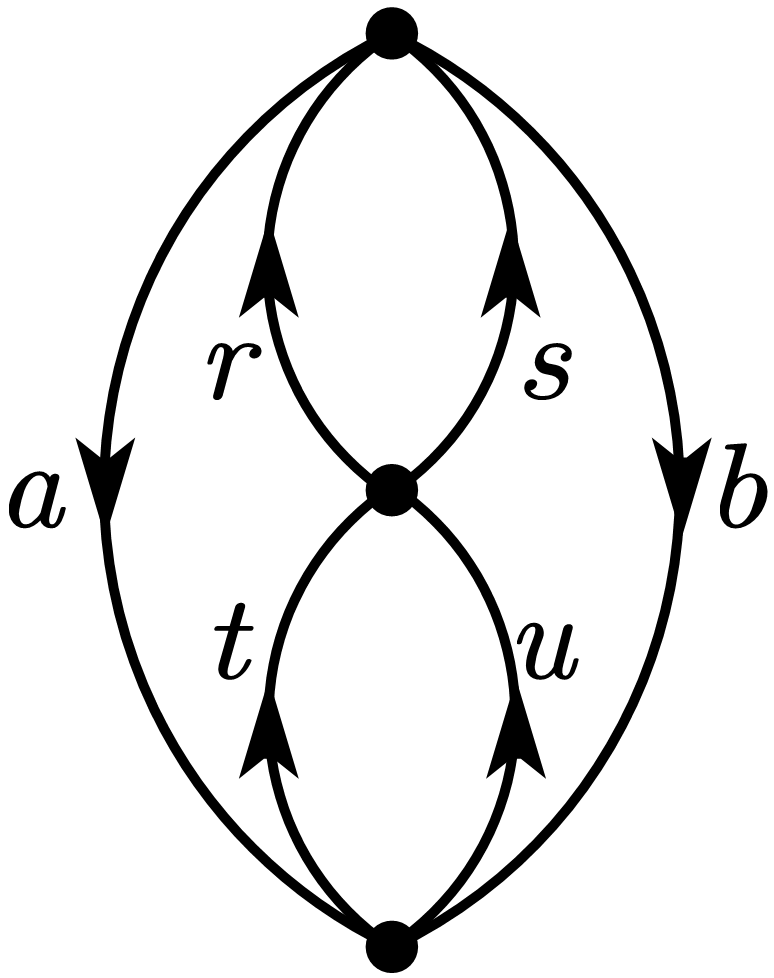
\includegraphics[scale=0.9]{./pictures/6.12/exercise_2.png}
	\end{center}
	
	Push all third-order diagrams in Table 6.2 together in a similar way and, thus, find which Goldstone diagram comes from which Hugenholtz diagram. For the above Hugenholtz diagram, verify that its mathematical value is indeed the sum of the values of the corresponding Goldstone diagrams.
	
	\end{exercise}
	
	\begin{solution}

	As the textbook mentioned at the page 361, there are three third-order Hugenholtz diagrams, which are listed in \Figref{fig:exe12_1}.

	\begin{center}
	\begin{tabular}{ccc}
	
		\begin{minipage}{0.22\linewidth}
		\centering
		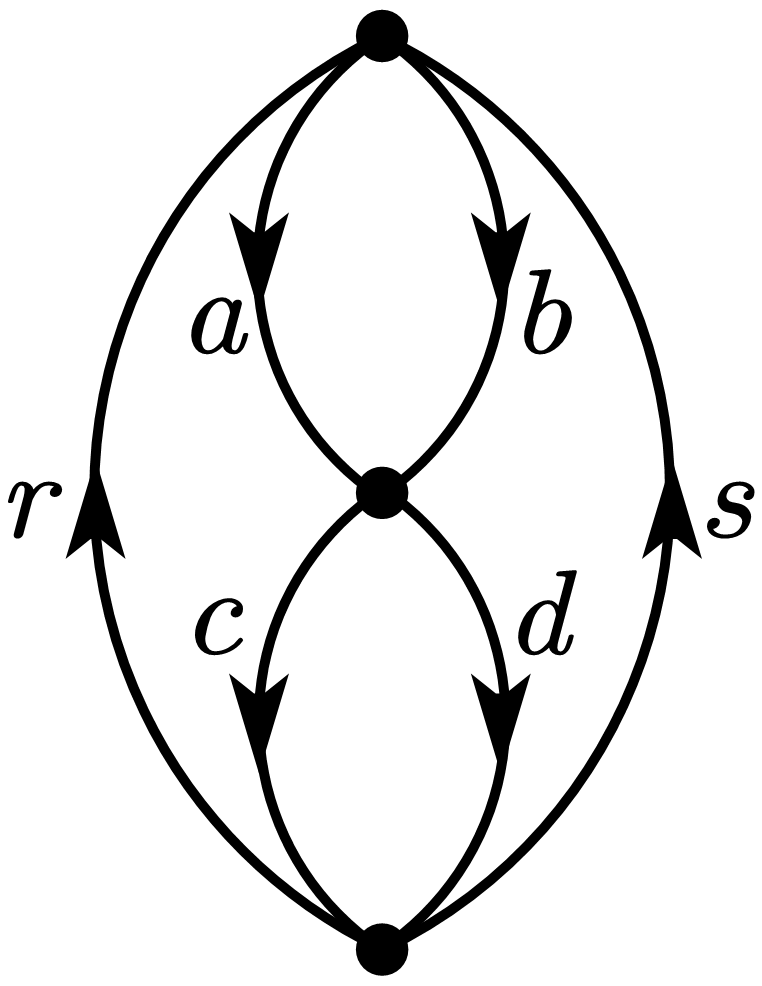
\includegraphics[scale=1.0,trim=0 -4 0 -4]{./pictures/6.12/hugenholtz_1.png}
		\end{minipage} &
		
		\begin{minipage}{0.22\linewidth}
		\centering
		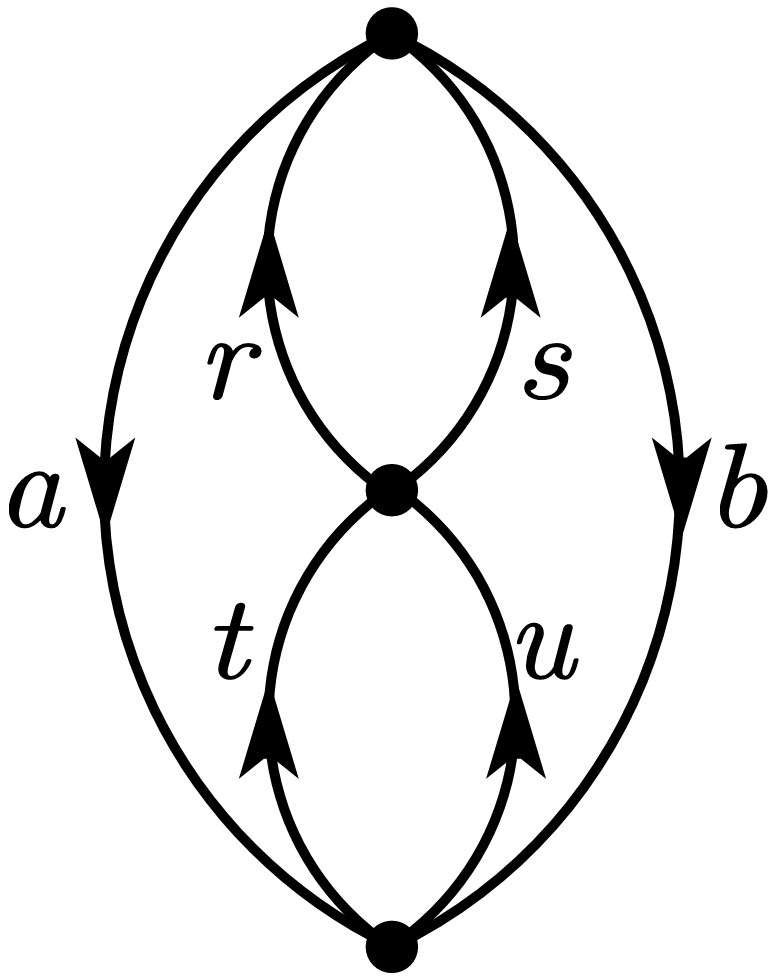
\includegraphics[scale=1.0,trim=0 -4 0 -4]{./pictures/6.12/hugenholtz_2.png}
		\end{minipage} &
		
		\begin{minipage}{0.22\linewidth}
		\centering
		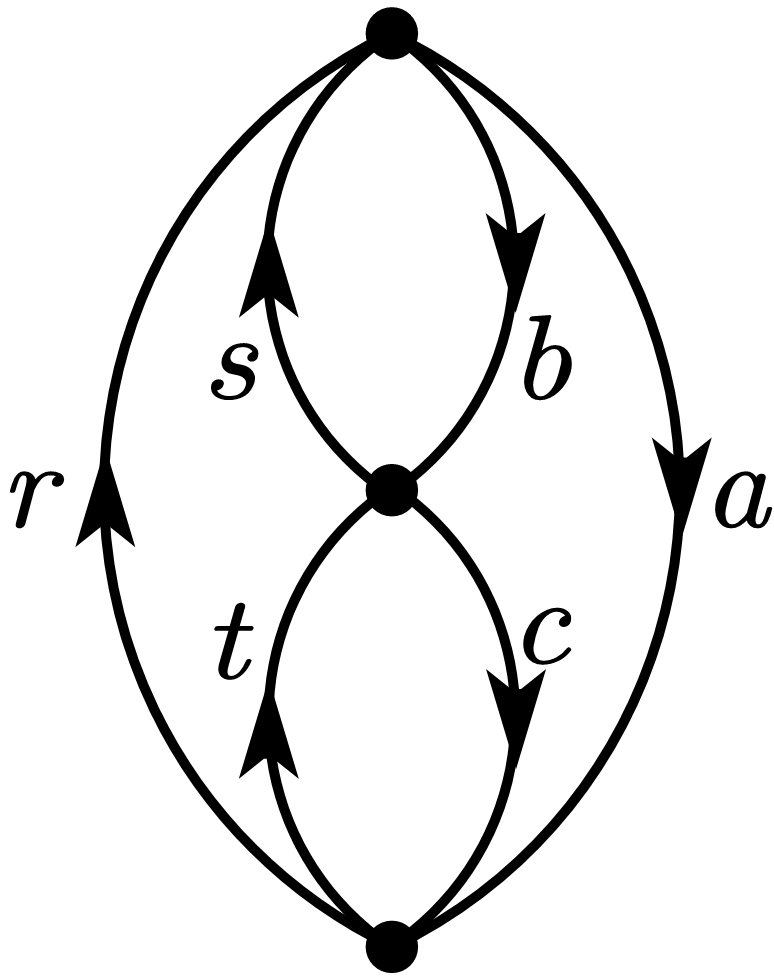
\includegraphics[scale=1.0,trim=0 -4 0 -4]{./pictures/6.12/hugenholtz_3.png}
		\end{minipage}
		
	\end{tabular}
	\captionof{figure}{All third-order Hugenholtz diagrams.}\label{fig:exe12_1}
	\end{center}
	
	In fact, the ``pushing together" results of these third-order Goldstone diagrams in the table 6.2 can be summarized as follows.
	\begin{itemize}
	
	\item Pushing together the second or the seventh third-order Goldstone diagrams leads to the first Hugenholtz diagram.
	
	\item Pushing together the first and the eighth third-order Goldstone diagrams leads to the second Hugenholtz diagram.
	
	\item Pushing together the rest of third-order Goldstone diagrams leads to the third Hugenholtz diagram.
	
	\end{itemize}
	
	Firstly, we will verify that the sum of the second and the seventh third-order Goldstone diagrams is the first third-order Hugenholtz diagram. The sum of the second and the seventh third-order Goldstone diagrams is
	\begin{align*}
		&\hspace{1.4em} (-1)^{4+2} \left( \frac{1}{2} \right) \sum_{abcdrs} \frac{ \langle ad | rs \rangle \langle cb | ad \rangle \langle rs | cb \rangle }{ ( \varepsilon_a + \varepsilon_d - \varepsilon_r - \varepsilon_s ) ( \varepsilon_c + \varepsilon_b - \varepsilon_r - \varepsilon_s ) } \\
		&\hspace{6em} + (-1)^{4+1} \left( \frac{1}{2} \right) \sum_{abcdrs} \frac{ \langle ac | rs \rangle \langle db | ac \rangle \langle sr | db \rangle }{ ( \varepsilon_a + \varepsilon_c - \varepsilon_r - \varepsilon_s ) ( \varepsilon_d + \varepsilon_b - \varepsilon_r - \varepsilon_s ) } \\
		&= \frac{1}{2} \sum_{abcdrs} \frac{ \langle ad | rs \rangle \langle cb | ad \rangle \langle rs | cb \rangle }{ ( \varepsilon_a + \varepsilon_d - \varepsilon_r - \varepsilon_s ) ( \varepsilon_c + \varepsilon_b - \varepsilon_r - \varepsilon_s ) } - \frac{ \langle ad | rs \rangle \langle cb | ad \rangle \langle sr | cb \rangle }{ ( \varepsilon_a + \varepsilon_d - \varepsilon_r - \varepsilon_s ) ( \varepsilon_c + \varepsilon_b - \varepsilon_r - \varepsilon_s ) } \\
		&= \frac{1}{2} \sum_{abcdrs} \frac{ \langle ad | rs \rangle \langle cb | ad \rangle \left( \langle rs | cb \rangle - \langle sr | cb \rangle \right) }{ ( \varepsilon_a + \varepsilon_d - \varepsilon_r - \varepsilon_s ) ( \varepsilon_c + \varepsilon_b - \varepsilon_r - \varepsilon_s ) } = \frac{1}{2} \sum_{abcdrs} \frac{ \langle ab | rs \rangle \langle cd | ab \rangle \left( \langle rs | cd \rangle - \langle sr | cd \rangle \right) }{ ( \varepsilon_a + \varepsilon_b - \varepsilon_r - \varepsilon_s ) ( \varepsilon_c + \varepsilon_d - \varepsilon_r - \varepsilon_s ) },
	\end{align*}
	and the first Hugenholtz diagram can be simplified to
	\begin{align*}
		&\hspace{1.4em} \frac{1}{8} \sum_{abcdrs} \frac{ \langle ab || rs \rangle \langle rs || cd \rangle \langle cd || ab \rangle }{ ( \varepsilon_a + \varepsilon_b - \varepsilon_r - \varepsilon_s ) ( \varepsilon_c + \varepsilon_d - \varepsilon_r - \varepsilon_s ) } \\
		&= \frac{1}{8} \sum_{abcdrs} \frac{ ( \langle ab | rs \rangle - \langle ab | sr \rangle )( \langle rs | cd \rangle - \langle rs | dc \rangle ) ( \langle cd | ab \rangle - \langle cd | ba \rangle ) }{ ( \varepsilon_a + \varepsilon_b - \varepsilon_r - \varepsilon_s ) ( \varepsilon_c + \varepsilon_d - \varepsilon_r - \varepsilon_s ) } \\
		&= \frac{1}{8} \sum_{abcdrs} \frac{ \langle ab | rs \rangle \langle rs | cd \rangle \langle cd | ab \rangle }{ ( \varepsilon_a + \varepsilon_b - \varepsilon_r - \varepsilon_s ) ( \varepsilon_c + \varepsilon_d - \varepsilon_r - \varepsilon_s ) } - \frac{ \langle ab | rs \rangle \langle rs | cd \rangle \langle cd | ba \rangle }{ ( \varepsilon_a + \varepsilon_b - \varepsilon_r - \varepsilon_s ) ( \varepsilon_c + \varepsilon_d - \varepsilon_r - \varepsilon_s ) } \\
		&\hspace{6em} - \frac{ \langle ab | rs \rangle \langle rs | dc \rangle \langle cd | ab \rangle }{ ( \varepsilon_a + \varepsilon_b - \varepsilon_r - \varepsilon_s ) ( \varepsilon_c + \varepsilon_d - \varepsilon_r - \varepsilon_s ) } + \frac{ \langle ab | rs \rangle \langle rs | dc \rangle \langle cd | ba \rangle }{ ( \varepsilon_a + \varepsilon_b - \varepsilon_r - \varepsilon_s ) ( \varepsilon_c + \varepsilon_d - \varepsilon_r - \varepsilon_s ) } \\
		&\hspace{6em} - \frac{ \langle ab | sr \rangle \langle rs | cd \rangle \langle cd | ab \rangle }{ ( \varepsilon_a + \varepsilon_b - \varepsilon_r - \varepsilon_s ) ( \varepsilon_c + \varepsilon_d - \varepsilon_r - \varepsilon_s ) } + \frac{ \langle ab | sr \rangle \langle rs | cd \rangle \langle cd | ba \rangle }{ ( \varepsilon_a + \varepsilon_b - \varepsilon_r - \varepsilon_s ) ( \varepsilon_c + \varepsilon_d - \varepsilon_r - \varepsilon_s ) } \\
		&\hspace{6em} + \frac{ \langle ab | sr \rangle \langle rs | dc \rangle \langle cd | ab \rangle }{ ( \varepsilon_a + \varepsilon_b - \varepsilon_r - \varepsilon_s ) ( \varepsilon_c + \varepsilon_d - \varepsilon_r - \varepsilon_s ) } - \frac{ \langle ab | sr \rangle \langle rs | dc \rangle \langle cd | ba \rangle }{ ( \varepsilon_a + \varepsilon_b - \varepsilon_r - \varepsilon_s ) ( \varepsilon_c + \varepsilon_d - \varepsilon_r - \varepsilon_s ) } \\
		&= \frac{1}{8} \sum_{abcdrs} \frac{ \langle ab | rs \rangle \langle cd | ab \rangle \langle rs | cd \rangle }{ ( \varepsilon_a + \varepsilon_b - \varepsilon_r - \varepsilon_s ) ( \varepsilon_c + \varepsilon_d - \varepsilon_r - \varepsilon_s ) } - \frac{ \langle ab | rs \rangle \langle rs | dc \rangle \langle dc | ba \rangle }{ ( \varepsilon_a + \varepsilon_b - \varepsilon_r - \varepsilon_s ) ( \varepsilon_c + \varepsilon_d - \varepsilon_r - \varepsilon_s ) } \\
		&\hspace{6em} - \frac{ \langle ab | rs \rangle \langle sr | cd \rangle \langle cd | ab \rangle }{ ( \varepsilon_a + \varepsilon_b - \varepsilon_r - \varepsilon_s ) ( \varepsilon_c + \varepsilon_d - \varepsilon_r - \varepsilon_s ) } + \frac{ \langle ab | rs \rangle \langle sr | dc \rangle \langle dc | ba \rangle }{ ( \varepsilon_a + \varepsilon_b - \varepsilon_r - \varepsilon_s ) ( \varepsilon_c + \varepsilon_d - \varepsilon_r - \varepsilon_s ) } \\
		&\hspace{6em} - \frac{ \langle ab | rs \rangle \langle sr | cd \rangle \langle cd | ab \rangle }{ ( \varepsilon_a + \varepsilon_b - \varepsilon_r - \varepsilon_s ) ( \varepsilon_c + \varepsilon_d - \varepsilon_r - \varepsilon_s ) } + \frac{ \langle ab | rs \rangle \langle sr | dc \rangle \langle dc | ba \rangle }{ ( \varepsilon_a + \varepsilon_b - \varepsilon_r - \varepsilon_s ) ( \varepsilon_c + \varepsilon_d - \varepsilon_r - \varepsilon_s ) } \\
		&\hspace{6em} + \frac{ \langle ab | rs \rangle \langle sr | dc \rangle \langle cd | ab \rangle }{ ( \varepsilon_a + \varepsilon_b - \varepsilon_r - \varepsilon_s ) ( \varepsilon_c + \varepsilon_d - \varepsilon_r - \varepsilon_s ) } - \frac{ \langle ab | rs \rangle \langle sr | cd \rangle \langle dc | ba \rangle }{ ( \varepsilon_a + \varepsilon_b - \varepsilon_r - \varepsilon_s ) ( \varepsilon_c + \varepsilon_d - \varepsilon_r - \varepsilon_s ) } \\
		&= \frac{1}{2} \sum_{abcdrs} \frac{ \langle ab | rs \rangle \langle cd | ab \rangle \left( \langle rs | cd \rangle - \langle sr | cd \rangle \right) }{ ( \varepsilon_a + \varepsilon_b - \varepsilon_r - \varepsilon_s ) ( \varepsilon_c + \varepsilon_d - \varepsilon_r - \varepsilon_s ) }.
	\end{align*}
	Thus, we have verified that the sum of the second and the seventh third-order Goldstone diagrams is the first third-order Hugenholtz diagram.
	
	Secondly, we will verify that the sum of the first and the eighth third-order Goldstone diagrams is the second third-order Hugenholtz diagram. The sum of the first and the eighth third-order Goldstone diagrams is
	\begin{align*}
		&(-1)^{2+2} \left( \frac{1}{2} \right) \sum_{abrsut} \frac{ \langle ab | ru \rangle \langle ru | ts \rangle \langle ts | ab \rangle }{ ( \varepsilon_a + \varepsilon_b - \varepsilon_r - \varepsilon_u ) ( \varepsilon_a + \varepsilon_b - \varepsilon_t - \varepsilon_s ) } \\
		&\hspace{6em}+ (-1)^{2+1} \left( \frac{1}{2} \right) \sum_{abrsut} \frac{ \langle ab | rt \rangle \langle tr | us \rangle \langle us | ab \rangle }{ ( \varepsilon_a + \varepsilon_b - \varepsilon_t - \varepsilon_r ) ( \varepsilon_a + \varepsilon_b - \varepsilon_u - \varepsilon_s ) } \\
		&= \frac{1}{2} \sum_{abrsut} \frac{ \langle ab | ru \rangle \langle ru | ts \rangle \langle ts | ab \rangle }{ ( \varepsilon_a + \varepsilon_b - \varepsilon_r - \varepsilon_u ) ( \varepsilon_a + \varepsilon_b - \varepsilon_t - \varepsilon_s ) } - \frac{ \langle ab | ru \rangle \langle ur | ts \rangle \langle ts | ab \rangle }{ ( \varepsilon_a + \varepsilon_b - \varepsilon_u - \varepsilon_r ) ( \varepsilon_a + \varepsilon_b - \varepsilon_t - \varepsilon_s ) } \\
		&= \frac{1}{2} \sum_{abrsut} \frac{ \langle ab | ru \rangle \langle ts | ab \rangle ( \langle ru | ts \rangle - \langle ur | ts \rangle ) }{ ( \varepsilon_a + \varepsilon_b - \varepsilon_r - \varepsilon_u ) ( \varepsilon_a + \varepsilon_b - \varepsilon_t - \varepsilon_s ) } = \frac{1}{2} \sum_{abrsut} \frac{ \langle ab | rs \rangle \langle tu | ab \rangle ( \langle rs | tu \rangle - \langle sr | tu \rangle ) }{ ( \varepsilon_a + \varepsilon_b - \varepsilon_r - \varepsilon_s ) ( \varepsilon_a + \varepsilon_b - \varepsilon_t - \varepsilon_u ) }.
	\end{align*}
	and the second Hugenholtz diagram can be simplified to
	\begin{align*}
		&\hspace{1.4em} \frac{1}{8} \sum_{abrstu} \frac{ \langle ab || rs \rangle \langle rs || tu \rangle \langle tu || ab \rangle }{ ( \varepsilon_a + \varepsilon_b - \varepsilon_r - \varepsilon_s ) ( \varepsilon_a + \varepsilon_b - \varepsilon_t - \varepsilon_u ) } \\
		&= \frac{1}{8} \sum_{abrstu} \frac{ ( \langle ab | rs \rangle - \langle ab | sr \rangle )( \langle rs | tu \rangle - \langle rs | ut \rangle ) ( \langle tu | ab \rangle - \langle tu | ba \rangle ) }{ ( \varepsilon_a + \varepsilon_b - \varepsilon_r - \varepsilon_s ) ( \varepsilon_a + \varepsilon_b - \varepsilon_t - \varepsilon_u ) } \\
		&= \frac{1}{8} \sum_{abrstu} \frac{ \langle ab | rs \rangle \langle rs | tu \rangle \langle tu | ab \rangle }{ ( \varepsilon_a + \varepsilon_b - \varepsilon_r - \varepsilon_s ) ( \varepsilon_a + \varepsilon_b - \varepsilon_t - \varepsilon_u ) } - \frac{ \langle ab | rs \rangle \langle rs | tu \rangle \langle tu | ba \rangle }{ ( \varepsilon_a + \varepsilon_b - \varepsilon_r - \varepsilon_s ) ( \varepsilon_a + \varepsilon_b - \varepsilon_t - \varepsilon_u ) } \\
		&\hspace{6em} - \frac{ \langle ab | rs \rangle \langle rs | ut \rangle \langle tu | ab \rangle }{ ( \varepsilon_a + \varepsilon_b - \varepsilon_r - \varepsilon_s ) ( \varepsilon_a + \varepsilon_b - \varepsilon_t - \varepsilon_u ) } + \frac{ \langle ab | rs \rangle \langle rs | ut \rangle \langle tu | ba \rangle }{ ( \varepsilon_a + \varepsilon_b - \varepsilon_r - \varepsilon_s ) ( \varepsilon_a + \varepsilon_b - \varepsilon_t - \varepsilon_u ) } \\
		&\hspace{6em} - \frac{ \langle ab | sr \rangle \langle rs | tu \rangle \langle tu | ab \rangle }{ ( \varepsilon_a + \varepsilon_b - \varepsilon_r - \varepsilon_s ) ( \varepsilon_a + \varepsilon_b - \varepsilon_t - \varepsilon_u ) } + \frac{ \langle ab | sr \rangle \langle rs | tu \rangle \langle tu | ba \rangle }{ ( \varepsilon_a + \varepsilon_b - \varepsilon_r - \varepsilon_s ) ( \varepsilon_a + \varepsilon_b - \varepsilon_t - \varepsilon_u ) } \\
		&\hspace{6em} + \frac{ \langle ab | sr \rangle \langle rs | ut \rangle \langle tu | ab \rangle }{ ( \varepsilon_a + \varepsilon_b - \varepsilon_r - \varepsilon_s ) ( \varepsilon_a + \varepsilon_b - \varepsilon_t - \varepsilon_u ) } - \frac{ \langle ab | sr \rangle \langle rs | ut \rangle \langle tu | ba \rangle }{ ( \varepsilon_a + \varepsilon_b - \varepsilon_r - \varepsilon_s ) ( \varepsilon_a + \varepsilon_b - \varepsilon_t - \varepsilon_u ) } \\
		&= \frac{1}{8} \sum_{abrstu} \frac{ \langle ab | rs \rangle \langle rs | tu \rangle \langle tu | ab \rangle }{ ( \varepsilon_a + \varepsilon_b - \varepsilon_r - \varepsilon_s ) ( \varepsilon_a + \varepsilon_b - \varepsilon_t - \varepsilon_u ) } - \frac{ \langle ab | rs \rangle \langle rs | ut \rangle \langle ut | ba \rangle }{ ( \varepsilon_a + \varepsilon_b - \varepsilon_r - \varepsilon_s ) ( \varepsilon_a + \varepsilon_b - \varepsilon_t - \varepsilon_u ) } \\
		&\hspace{6em} - \frac{ \langle ab | rs \rangle \langle rs | tu \rangle \langle ut | ab \rangle }{ ( \varepsilon_a + \varepsilon_b - \varepsilon_r - \varepsilon_s ) ( \varepsilon_a + \varepsilon_b - \varepsilon_t - \varepsilon_u ) } + \frac{ \langle ab | rs \rangle \langle rs | tu \rangle \langle ut | ba \rangle }{ ( \varepsilon_a + \varepsilon_b - \varepsilon_r - \varepsilon_s ) ( \varepsilon_a + \varepsilon_b - \varepsilon_t - \varepsilon_u ) } \\
		&\hspace{6em} - \frac{ \langle ab | rs \rangle \langle sr | tu \rangle \langle tu | ab \rangle }{ ( \varepsilon_a + \varepsilon_b - \varepsilon_r - \varepsilon_s ) ( \varepsilon_a + \varepsilon_b - \varepsilon_t - \varepsilon_u ) } + \frac{ \langle ab | rs \rangle \langle sr | ut \rangle \langle ut | ba \rangle }{ ( \varepsilon_a + \varepsilon_b - \varepsilon_r - \varepsilon_s ) ( \varepsilon_a + \varepsilon_b - \varepsilon_t - \varepsilon_u ) } \\
		&\hspace{6em} + \frac{ \langle ab | rs \rangle \langle sr | ut \rangle \langle tu | ab \rangle }{ ( \varepsilon_a + \varepsilon_b - \varepsilon_r - \varepsilon_s ) ( \varepsilon_a + \varepsilon_b - \varepsilon_t - \varepsilon_u ) } - \frac{ \langle ab | rs \rangle \langle sr | tu \rangle \langle ut | ba \rangle }{ ( \varepsilon_a + \varepsilon_b - \varepsilon_r - \varepsilon_s ) ( \varepsilon_a + \varepsilon_b - \varepsilon_t - \varepsilon_u ) } \\
		&= \frac{1}{2} \sum_{abrstu} \frac{ \langle ab | rs \rangle \langle rs | tu \rangle \langle tu | ab \rangle }{ ( \varepsilon_a + \varepsilon_b - \varepsilon_r - \varepsilon_s ) ( \varepsilon_a + \varepsilon_b - \varepsilon_t - \varepsilon_u ) } - \frac{ \langle ab | rs \rangle \langle rs | ut \rangle \langle ut | ba \rangle }{ ( \varepsilon_a + \varepsilon_b - \varepsilon_r - \varepsilon_s ) ( \varepsilon_a + \varepsilon_b - \varepsilon_t - \varepsilon_u ) } \\
		&= \frac{1}{2} \sum_{abrsut} \frac{ \langle ab | rs \rangle \langle tu | ab \rangle ( \langle rs | tu \rangle - \langle sr | tu \rangle ) }{ ( \varepsilon_a + \varepsilon_b - \varepsilon_r - \varepsilon_s ) ( \varepsilon_a + \varepsilon_b - \varepsilon_t - \varepsilon_u ) }.
	\end{align*}
	Thus, we have verified that the sum of the first and the eighth third-order Goldstone diagrams is the second third-order Hugenholtz diagram.
	
	Thirdly, we will verify that the sum of the rest of third-order Goldstone diagrams is the third third-order Hugenholtz diagram. The third third-order Hugenholtz diagram is	
	\begin{align*}
		&\hspace{1.4em}\sum_{abcrst} \frac{ \langle ab || rs \rangle \langle cs || tb \rangle \langle rt || ac \rangle }{ ( \varepsilon_a + \varepsilon_b - \varepsilon_s - \varepsilon_r ) ( \varepsilon_a + \varepsilon_c - \varepsilon_r - \varepsilon_t ) } \\
		&= \sum_{abcrst} \frac{ [ \langle ab | rs \rangle - \langle ab | sr \rangle ] [ \langle cs | tb \rangle - \langle cs | bt \rangle ] [ \langle rt | ac \rangle - \langle rt | ca \rangle ] }{ ( \varepsilon_a + \varepsilon_b - \varepsilon_s - \varepsilon_r ) ( \varepsilon_a + \varepsilon_c - \varepsilon_r - \varepsilon_t ) } \\
		&= \sum_{abcrst} \frac{ \langle ab | rs \rangle \langle cs | tb \rangle \langle rt | ac \rangle }{ ( \varepsilon_a + \varepsilon_b - \varepsilon_r - \varepsilon_s ) ( \varepsilon_a + \varepsilon_c - \varepsilon_r - \varepsilon_t ) } - \frac{ \langle ab | rs \rangle \langle cs | tb \rangle \langle rt | ca \rangle }{ ( \varepsilon_a + \varepsilon_b - \varepsilon_r - \varepsilon_s ) ( \varepsilon_a + \varepsilon_c - \varepsilon_r - \varepsilon_t ) } \\
		&\hspace{4em} - \frac{ \langle ab | rs \rangle \langle cs | bt \rangle \langle rt | ac \rangle }{ ( \varepsilon_a + \varepsilon_b - \varepsilon_r - \varepsilon_s ) ( \varepsilon_a + \varepsilon_c - \varepsilon_r - \varepsilon_t ) } + \frac{ \langle ab | rs \rangle \langle cs | bt \rangle \langle rt | ca \rangle }{ ( \varepsilon_a + \varepsilon_b - \varepsilon_r - \varepsilon_s ) ( \varepsilon_a + \varepsilon_c - \varepsilon_r - \varepsilon_t ) } \\
		&\hspace{4em} - \frac{ \langle ab | sr \rangle \langle cs | tb \rangle \langle rt | ac \rangle }{ ( \varepsilon_a + \varepsilon_b - \varepsilon_r - \varepsilon_s ) ( \varepsilon_a + \varepsilon_c - \varepsilon_r - \varepsilon_t ) } + \frac{ \langle ab | sr \rangle \langle cs | tb \rangle \langle rt | ca \rangle }{ ( \varepsilon_a + \varepsilon_b - \varepsilon_r - \varepsilon_s ) ( \varepsilon_a + \varepsilon_c - \varepsilon_r - \varepsilon_t ) } \\
		&\hspace{4em} + \frac{ \langle ab | sr \rangle \langle cs | bt \rangle \langle rt | ac \rangle }{ ( \varepsilon_a + \varepsilon_b - \varepsilon_r - \varepsilon_s ) ( \varepsilon_a + \varepsilon_c - \varepsilon_r - \varepsilon_t ) } - \frac{ \langle ab | sr \rangle \langle cs | bt \rangle \langle rt | ca \rangle }{ ( \varepsilon_a + \varepsilon_b - \varepsilon_r - \varepsilon_s ) ( \varepsilon_a + \varepsilon_c - \varepsilon_r - \varepsilon_t ) } \\
		&= \sum_{abcrst} \frac{ \langle ac | rt \rangle \langle bt | sc \rangle \langle rs | ab \rangle }{ ( \varepsilon_a + \varepsilon_c - \varepsilon_r - \varepsilon_t ) ( \varepsilon_a + \varepsilon_b - \varepsilon_r - \varepsilon_s ) } - \frac{ \langle bc | rt \rangle \langle at | sc \rangle \langle rs | ab \rangle }{ ( \varepsilon_b + \varepsilon_c - \varepsilon_t - \varepsilon_r ) ( \varepsilon_a + \varepsilon_b - \varepsilon_r - \varepsilon_s ) } \\
		&\hspace{2em} - \sum_{abcrst} \frac{ \langle bc | rt \rangle \langle ra | sb \rangle \langle st | ac \rangle }{ ( \varepsilon_b + \varepsilon_c - \varepsilon_r - \varepsilon_t ) ( \varepsilon_a + \varepsilon_c - \varepsilon_s - \varepsilon_t ) } + \sum_{abcrst} \frac{ \langle bc | rt \rangle \langle ar | bs \rangle \langle ts | ac \rangle }{ ( \varepsilon_c + \varepsilon_b - \varepsilon_r - \varepsilon_t ) ( \varepsilon_a + \varepsilon_c - \varepsilon_s - \varepsilon_t ) } \\
		&\hspace{2em} - \sum_{abcrst} \frac{ \langle ab | rs \rangle \langle sc | at \rangle \langle rt | bc \rangle }{ ( \varepsilon_a + \varepsilon_b - \varepsilon_r - \varepsilon_s ) ( \varepsilon_c + \varepsilon_b - \varepsilon_r - \varepsilon_t ) } + \sum_{abcrst} \frac{ \langle cb | rt \rangle \langle at | sc \rangle \langle rs | ab \rangle }{ ( \varepsilon_c + \varepsilon_b - \varepsilon_r - \varepsilon_t ) ( \varepsilon_a + \varepsilon_b - \varepsilon_r - \varepsilon_s ) } \\
		&\hspace{2em} + \sum_{abcrst} \frac{ \langle cb | rt \rangle \langle ra | sb \rangle \langle st | ac \rangle }{ ( \varepsilon_c + \varepsilon_b - \varepsilon_r - \varepsilon_t ) ( \varepsilon_a + \varepsilon_c - \varepsilon_s - \varepsilon_t ) } - \sum_{abcrst} \frac{ \langle ac | rt \rangle \langle rb | sc \rangle \langle st | ab \rangle }{ ( \varepsilon_a + \varepsilon_c - \varepsilon_r - \varepsilon_t ) ( \varepsilon_a + \varepsilon_b - \varepsilon_s - \varepsilon_t ) }.
	\end{align*}	
	These eight terms correspond to the fifth, twelfth, fourth, ninth, eleventh, sixth, tenth, third third-order Goldstone diagrams, respectively.
	
	In conclusion, we have verified that the first third-order Hugenholtz diagram corresponds the second and the seventh third-order Goldstone diagrams, the second third-order Hugenholtz diagram corresponds the first and the eighth third-order Goldstone diagrams, and the third third-order Hugenholtz diagram corresponds the third, fourth, fifth, sixth, ninth, tenth, eleventh, twelfth third-order Goldstone diagrams.
	\end{solution}
	
	\subsection{Summation of Diagrams}
	
	\subsection{What Is the Linked Cluster Theorem?}
	
	% 6.13
	\begin{exercise}
	Calculate $E^{(3)}_0$ for a supermolecule consisting of $N$ non-interacting minimal basis $\ce{H2}$ molecules by evaluating the Goldstone diagrams in Table 6.2. Compare your result with that of Eq.(6.92), which was obtained algebraically by explicitly cancelling terms proportional to $N^2$.
	
	{\it Hint}: Simply show that the value of each Goldstone diagram for the supermolecule in $N$ times the result for a single molecule.
	\end{exercise}
	
	\begin{solution}
	Note that in this model, all two-electron integrals involving orbitals from different units are zero, and all third-order terms in the table 6.2 will be zero unless their numerators are non-zero. Thus, each third-order term of this model is just the sum of that of each units, leading that the value of each Goldstone diagram for the supermolecule in $N$ times the result for a single molecule.
	\end{solution}
	
	\section{Some Illustrative Calculations}

\end{document}